% Template for Carleton student papers
% Author: Andrew Gainer-Dewar, 2013
% This work is licensed under the Creative Commons Attribution 4.0 International License.
% To view a copy of this license, visit http://creativecommons.org/licenses/by/4.0/ or send a letter to Creative Commons, 444 Castro Street, Suite 900, Mountain View, California, 94041, USA.
\documentclass[12pt,twoside,letterpaper]{article}
\usepackage[style=apa, backend=biber, natbib=true, language=american]{biblatex}
\usepackage[T1]{fontenc}
\usepackage{nicematrix}
\usepackage{ragged2e}
\DeclareLanguageMapping{american}{american-apa}
% \renewcommand*{\nameyeardelim}{\addcomma\space}
\renewcommand*{\postnotedelim}{\addsemicolon\space}

\newrobustcmd*{\postcite}[1]{%
  \nocite{#1}\entrydata{#1}{\usebibmacro{cite}}
  }
\newrobustcmd*{\postcitemult}[2]{%
\nocite{#1}\entrydata{#1}{\usebibmacro{cite}},
\nocite{#2}\entrydata{#2}{\usebibmacro{cite}}
}
\usepackage{nicematrix}

% % APA-specific adjustments
% \AtBeginBibliography{\renewcommand*{\mkbibnamefamily}[1]{\textsc{#1}}} % APA-style author capitalization in bibliography

% % Other biblatex adjustments to mimic APA style
% \DeclareNameAlias{sortname}{last-first} % Last name, first name format
% \DeclareNameAlias{default}{last-first}

\addbibresource{sources.bib}
% % Add a comma between author and year for in-text citations
% \renewcommand{\nameyeardelim}{\addcomma\space}
% \newcommand{\texteq}[2][0.5]{\text{\parbox[t]{#1\displaywidth}{#2}}}
% \newcommand{\lther}{\mathord{\therefore}\mskip\thickmuskip}
%-----------------------------------------------------------------
% Lengths to control indents of 'equation numbers' and statements
% \newlength{\numbersep}          % Distance of number at left margin
% \newlength{\statementsep}       % Distance of statement at left margin
% \setlength{\numbersep}{\parindent}  % n
% \setlength{\statementsep}{15mm}    % m (0<n<m) 
%-----------------------------------------------------------------
% \everydisplay{\displayindent=\numbersep}
% \setlength{\mathindent}{\statementsep}
% \setlength{\mathindent}{3cm}
\usepackage{ccpaper}
\usepackage{setspace, graphicx, caption} %\doublespacing
\usepackage{geometry, tikz, nccmath, graphbox}
\usepackage{tikzsymbols}
\usepackage{gensymb,algorithm2e}
\RestyleAlgo{ruled}
\allowdisplaybreaks
\geometry{portrait, margin=1in}
\usepackage[title]{appendix}
\usetikzlibrary{shapes.geometric}
\usetikzlibrary{arrows.meta,arrows}
\usetikzlibrary{positioning}
% \usepackage{cite}
% The Latin Modern font is a modernized replacement for the classic
% Computer Modern. Feel free to replace this with a different font package.
\usepackage{lmodern}
\usepackage{preamble2}
\newcommand{\Bias}[2]{\text{Bias}_{\text{#2}} \left(#1\right)}


% \makeatletter
% \newcommand{\myitem}[1]{%
% \item[#1]\protected@edef\@currentlabel{#1}%
% }
% \makeatother

% Define a new item command with custom labels and references
\newlist{myenumerate}{enumerate}{1}
\setlist[myenumerate,1]{
    label={\theenumi.},     % Labels will include dots (e.g., P1., C1., etc.)
    ref={\theenumi},
    leftmargin=*,       % Indent matches paragraph indentation
    labelindent=1.6\parindent
    % ,
    % widest=P8,              % Adjusts width to align with the widest label (optional)
}

% Customize counters for P and C items
\makeatletter
\newcommand{\myitem}[1]{%
    \item[\textbf{#1.}]%
    \def\@currentlabel{#1}% Set the label for referencing
}
\makeatother

\makeatletter
\newcommand{\myitemA}[1]{%
    \item[$\mathbf{#1:}$]%
    \def\@currentlabel{$\mathbf{#1}$}% Set the label for referencing
}
\makeatother

\makeatletter
\newcommand{\myitemB}[1]{%
    \item[$#1:$]%
    \def\@currentlabel{$\#1$}% Set the label for referencing
}
\makeatother

% Load in biblatex
% To use a different bibliography style, just change "numeric" to
% your pautoreferred style (mla for MLA style, alphabetic for Author-Year
% style, etc.) There are a lot of options; check the BibLaTeX documentation.
% \usepackage{natbib}

% Select the bibliography file
\usepackage{csquotes}
\usepackage{coffee4}
%Use single spacing, set 10pt font, set italics, and beginning quotes
% \renewcommand{\mkbegdispquote}
%     {\selectfont\textooquote}%\setquotestyle{quote}
% %End displayquote environment with ending quotes
% \renewcommand{\mkenddispquote}{\textcoquote}

\title{\textbf{LA Nurse BP}}
\subtitle{Case Study 1\footnote{Code used for this project is available at this \href{https://github.com/kwlyu/stat330-w25-case-study-1.git}{GitHub Repository}.}} %Optional. Omit if not wanted.
\author{Kunwu Lyu}
\date{Feburary 13, 2025}

\prof{Katie St. Clair}
\course{STAT 330}
\usepackage{epigraph}
\setlength\epigraphwidth{.8\textwidth}
\setlength\epigraphrule{0pt}
\renewcommand*{\bibfont}{\normalfont \small}
% \usepackage{etoolbox}
% \apptocmd{\thebibliography}{\interlinepenalty 1000000\relax}{}{}
% To enable double spacing, uncomment this line:
\titlespacing*{\section}
{0pt}{0ex}{0ex}
\titlespacing*{\subsection}
{0pt}{0ex}{0ex}
\usepackage{sectsty}
\sectionfont{\fontsize{12}{12}\selectfont}
\subsectionfont{\fontsize{12}{12}\selectfont}

\theoremstyle{definition}
\newtheorem{theorem}{Theorem}[section]
\newtheorem{corollary}{Corollary}[theorem]
\newtheorem{lemma}{Lemma}[theorem]
\theoremstyle{definition}
\newtheorem{definition}{Definition}[section]
\usepackage{xpatch}
\xpatchcmd{\NCC@ignorepar}{%
\abovedisplayskip\abovedisplayshortskip}
{%
\abovedisplayskip\abovedisplayshortskip%
\belowdisplayskip\belowdisplayshortskip}
{}{}

\usepackage{verbatim}
\newcommand{\detailtexcount}[1]{ %
\immediate\write18{texcount -merge -sum #1.tex > #1.wcdetail }%
\verbatiminput{#1.wcdetail}%
}

% \usepackage{verbatim}

% \newcommand{\detailtexcount}[1]{%
%   \immediate\write18{texcount -merge -sum -q #1. > #1.wcdetail }%
%   \verbatiminput{#1.wcdetail}%
% }
% Reduce space before and after the array environment
\setlength{\abovedisplayskip}{0pt}
\setlength{\belowdisplayskip}{0pt}
% \setcounter{section}{-1}
% Reduce space in enumerate environment
\setlist{nosep}
\begin{document}
\renewcommand{\abstractname}{Executive Summary}
\maketitle{\vspace{-6ex}}
% \setlength{\parskip}{0.2cm}
% \setlength{\mathindent}{31pt}
\expandafter\def\expandafter\normalsize\expandafter{%
    \normalsize%
    \setlength\abovedisplayskip{0pt}%
    \setlength\belowdisplayskip{0pt}%
    \setlength\abovedisplayshortskip{0pt}%
    \setlength\belowdisplayshortskip{0pt}%
}
% \cofeAm{0.4}{0.8}{0}{5.5cm}{9cm}
% \doublespacing
\singlespacing

\begin{abstract}
    Here is what I did.
\end{abstract}

\section{Introduction}\label{sec: intro}

Certain traits such as family history and mood are expected to increase one's ambulatory blood pressure (BP). \citet{goldstein_ambulatory_2000} studied potential factors that contribute to hypertension. They collected information about the participants' BP, activity levels, work status, and mood ratings throughout the day, as well as relevant family history and information about their menstrual phases, to establish links that lead to elevated BP. Towards the end, they sought to uncover preventative measures for individuals who may be at a higher risks of developing hypertension. The objectives of this project is much simpler. I am interested in exactly what traits are \emph{associated} with elevating one's BP, given the longitudinal structure and various time-dependent metrics in the dataset \parencites(given by)()[cited by \postcite{roback_beyond_2021}]{goldstein_ambulatory_2000}.

\subsection{Methods}\label{sec: method}

The dataset includes repeated measures over the course of two work and off-work days on 203 registered nurses between the ages of 24 and 50 years working in Los Angeles, in the year 2000. Of those 203 nurses, 172 has complete data on all of the variables recorded.\footnote{In the original paper by Goldstein and Shapiro \pnotecite[228-29]{goldstein_ambulatory_2000}, they reported 171 nurses who completed all sessions. It is likely that this is due to \citet{roback_beyond_2021} or \citet{weiss_modeling_2005} excluding other personality variables used in the original study. Because I am not investigating personality traits in this project, 172 suffices being my total subject counts. Additionally, Goldstein and Shapiro  mention that ``[s]imilar patterns of findings were obtained in the sample of 171 as in the total sample'' \pnotecite[229]{goldstein_ambulatory_2000}.} BP of the participants were measured 30 minutes before their normal start of work, and measured measured repeatedly every 20 minutes for the rest of the day. This led to around 40-60 observations per nurse (9573 total observations). Each time the BP was taken, participants were asked to give several mood ratings including happiness, stress, and tiredness. In addition, participants wore an actigraph on their waist to record frequency of movements in one-minute intervals; the researchers obtained an activity measure for the ten-minute periods before each BP reading.

\section{Exploratory Data Analysis}\label{sec: eda}

The variables (original and re-parameterized) used in this project are given in \Cref{tab: var desc}. Variable missingness was explored in \Cref{fig: missing}. We see that the data were missing primarily mood ratings and some activity levels from several participants. Because I am interested in how both of these variables relate to BP, I will proceed the analysis with the missing rows removed, leaving us with a total of 172 participants and 7877 observations. The visuals and statistics below will be given in terms of that subset of the data, unless otherwise specified.

\begin{table} 
    \centering\begin{tabular}{|p{0.2\linewidth} | p{0.65\linewidth}|}
        \hline
        Variable Name & Variable Descrption \\
        \hline\hline
        ID (Cluster) & Unique identification number for each participant \\
        \hline
        BP (Response) & Systolic blood pressure (in mmHg) \\
        \hline
        \textcolor[RGB]{208, 2, 27}{Act} & Activity level (frequency of movements in 1-minute intervals, over a 10-minute period) \\
        \hline
        \textcolor[RGB]{74, 144, 226}{Phase} & Menstrual phase (follicular or luteal) \\
        \hline
        \textcolor[RGB]{74, 144, 226}{Day} & Workday or non-workday \\
        \hline
        \textcolor[RGB]{208, 2, 27}{Posture} & Position during BP measurement (sitting, standing, or reclining) \\
        \hline
        \textcolor[RGB]{208, 2, 27}{HAP} & Self-ratings of happiness by each nurse at the time of each BP measurement on a 5-point scale (5 strongest and 1 weakest) \\
        \hline
        \textcolor[RGB]{208, 2, 27}{STR} & Self-ratings of stress by each nurse at the time of each BP measurement on a 5-point scale (5 strongest and 1 weakest) \\
        \hline
        \textcolor[RGB]{208, 2, 27}{TIR} & Self-ratings of tiredness by each nurse at the time of each BP measurement on a 5-point scale (5 strongest and 1 weakest) \\
        \hline
        \textcolor[RGB]{74, 144, 226}{Age} & Age (in years) \\
        \hline
        \textcolor[RGB]{74, 144, 226}{Full FH} & Family history, coded as either NO (no family history of  hypertension), YES (1 hypertensive parent), or YESYES (both parents hypertensive) \\
        \textcolor[RGB]{208, 2, 27}{Timepass} & Number of minutes since the first measurement \\
        \hline
        \hline\hline
        \emph{\textcolor[RGB]{208, 2, 27}{Stand}} & Indicator variable for standing, where it equals 0 if Posture is either sitting or reclining and 1 when Posture is standing \\
        \hline
        \emph{\textcolor[RGB]{208, 2, 27}{Mood}} & Combined mood ratings: HAP - (STR + TIR)/2 \\
        \hline
        \emph{\textcolor[RGB]{74, 144, 226}{FH}} & Indicator variable for having family history of hypertension (1 for YES and YESYES, 0 for NO) \\
        \hline
        \emph{\textcolor[RGB]{74, 144, 226}{Age24}} & Recentered Age: Age - 24 \\
        \hline
        \multicolumn{2}{c}{\footnotesize Note: \emph{emphasis} added to re-parameterized variables; colors represent levels.}
    \end{tabular}
    \caption{Variable Descrptions}
    \label{tab: var desc}
\end{table}

\begin{figure}
\centering
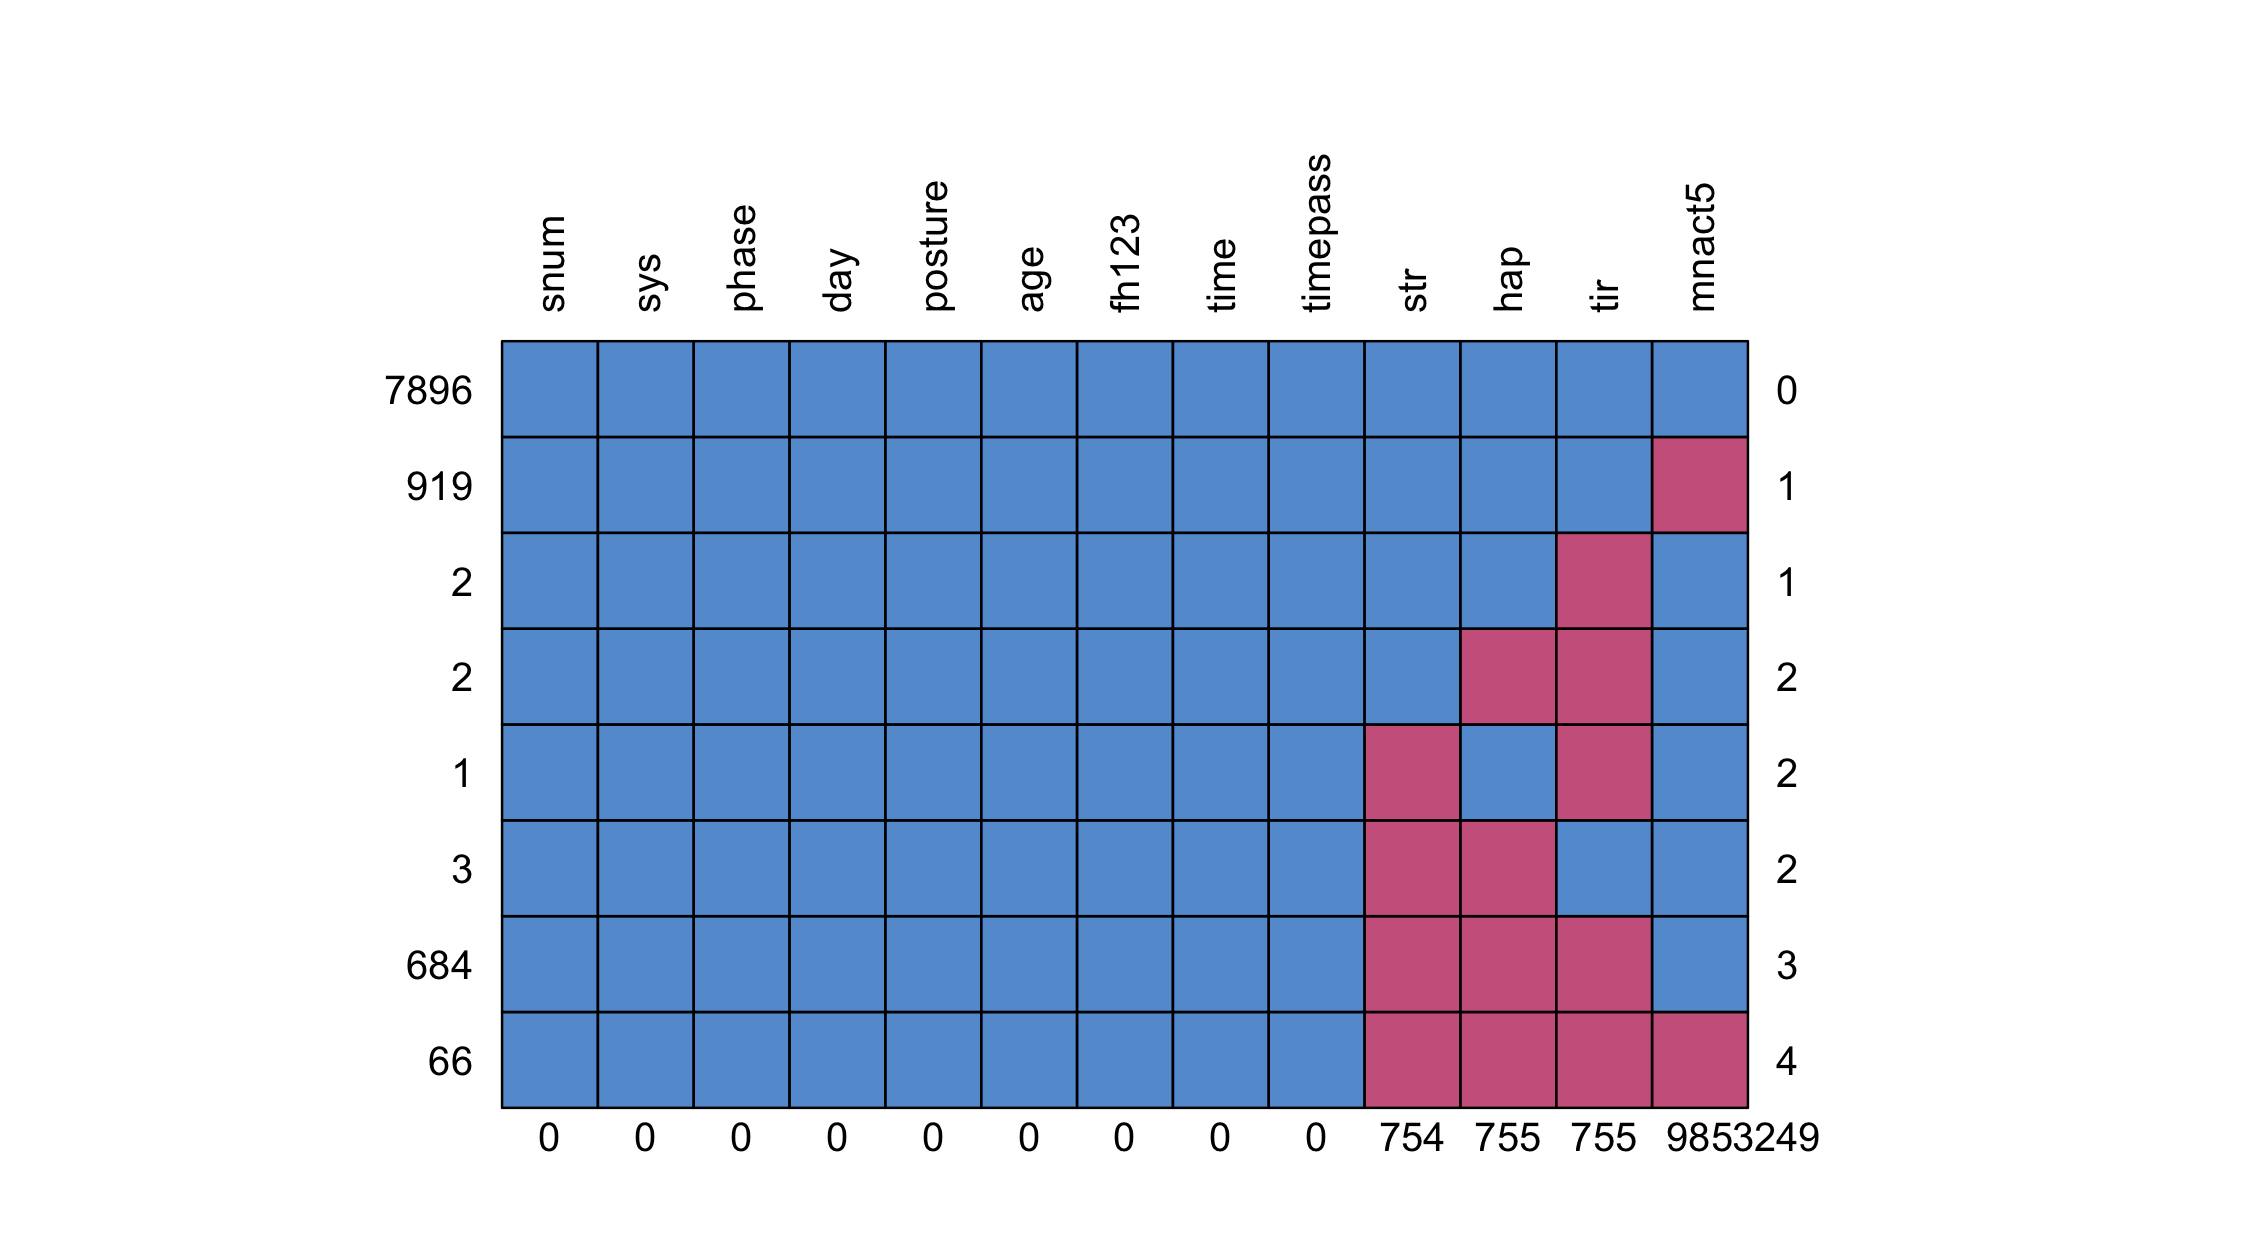
\includegraphics[width=\textwidth]{pics/miss.png}
\caption{Data Missingness}
\label{fig: missing}
\end{figure}

Because of the longitudinal nature of our data, it is worth noting our levels of analysis and to which our variables belong. I will call time-dependent measurements \emph{\textcolor[RGB]{208, 2, 27}{Level 1}} data (variables) and the rest of the subject-level measurements \emph{\textcolor[RGB]{74, 144, 226}{Level 2}} data (variables). Each participant has a unique identification number; this will distinguish between different clusters. Our primary response is systolic blood pressure (BP), and I will use our exploratory data analysis below to guide our model selection process from the bottom-up.

Note that I created three additional variables from the original dataset to help simplify the modeling process. In the original dataset, \texttt{Posture} is a factor variable with three levels: Recline ($n = 530$), Sit ($n = 3644$), and Stand ($n = 3703$). Because the relatively small number of observations where participants were reclining (presumably sleeping at night or resting), I collapsed the three levels into either Standing or non-Standing. Similarly, because of the relatively small number of participants have both parents with hypertension ($n = 13$), I collapsed it together with having one parent with hypertension ($n = 66$) to compare against those without any family history ($n = 103$). Lastly, a general \texttt{Mood} measurement was created by subtracting the average of tiredness and stress from happiness. 

\subsection{Level 1 by Clusters}\label{sec: lv1}

I will first explore how BP vary among participants and how it relates to the level 1 predictors to examine if there is any sign of clustering between different participants (which is the premise of a longitudinal study). From \Cref{fig: bp by subjects}, we see that BP readings do tend to vary among different participants, though variations within each participant do not seem to be pronounced. This suggests that a Linear Mixed Model (LMM) might be more appropriate than a regular Multiple Linear Regression (MLR).

\begin{figure} 
    \centering
    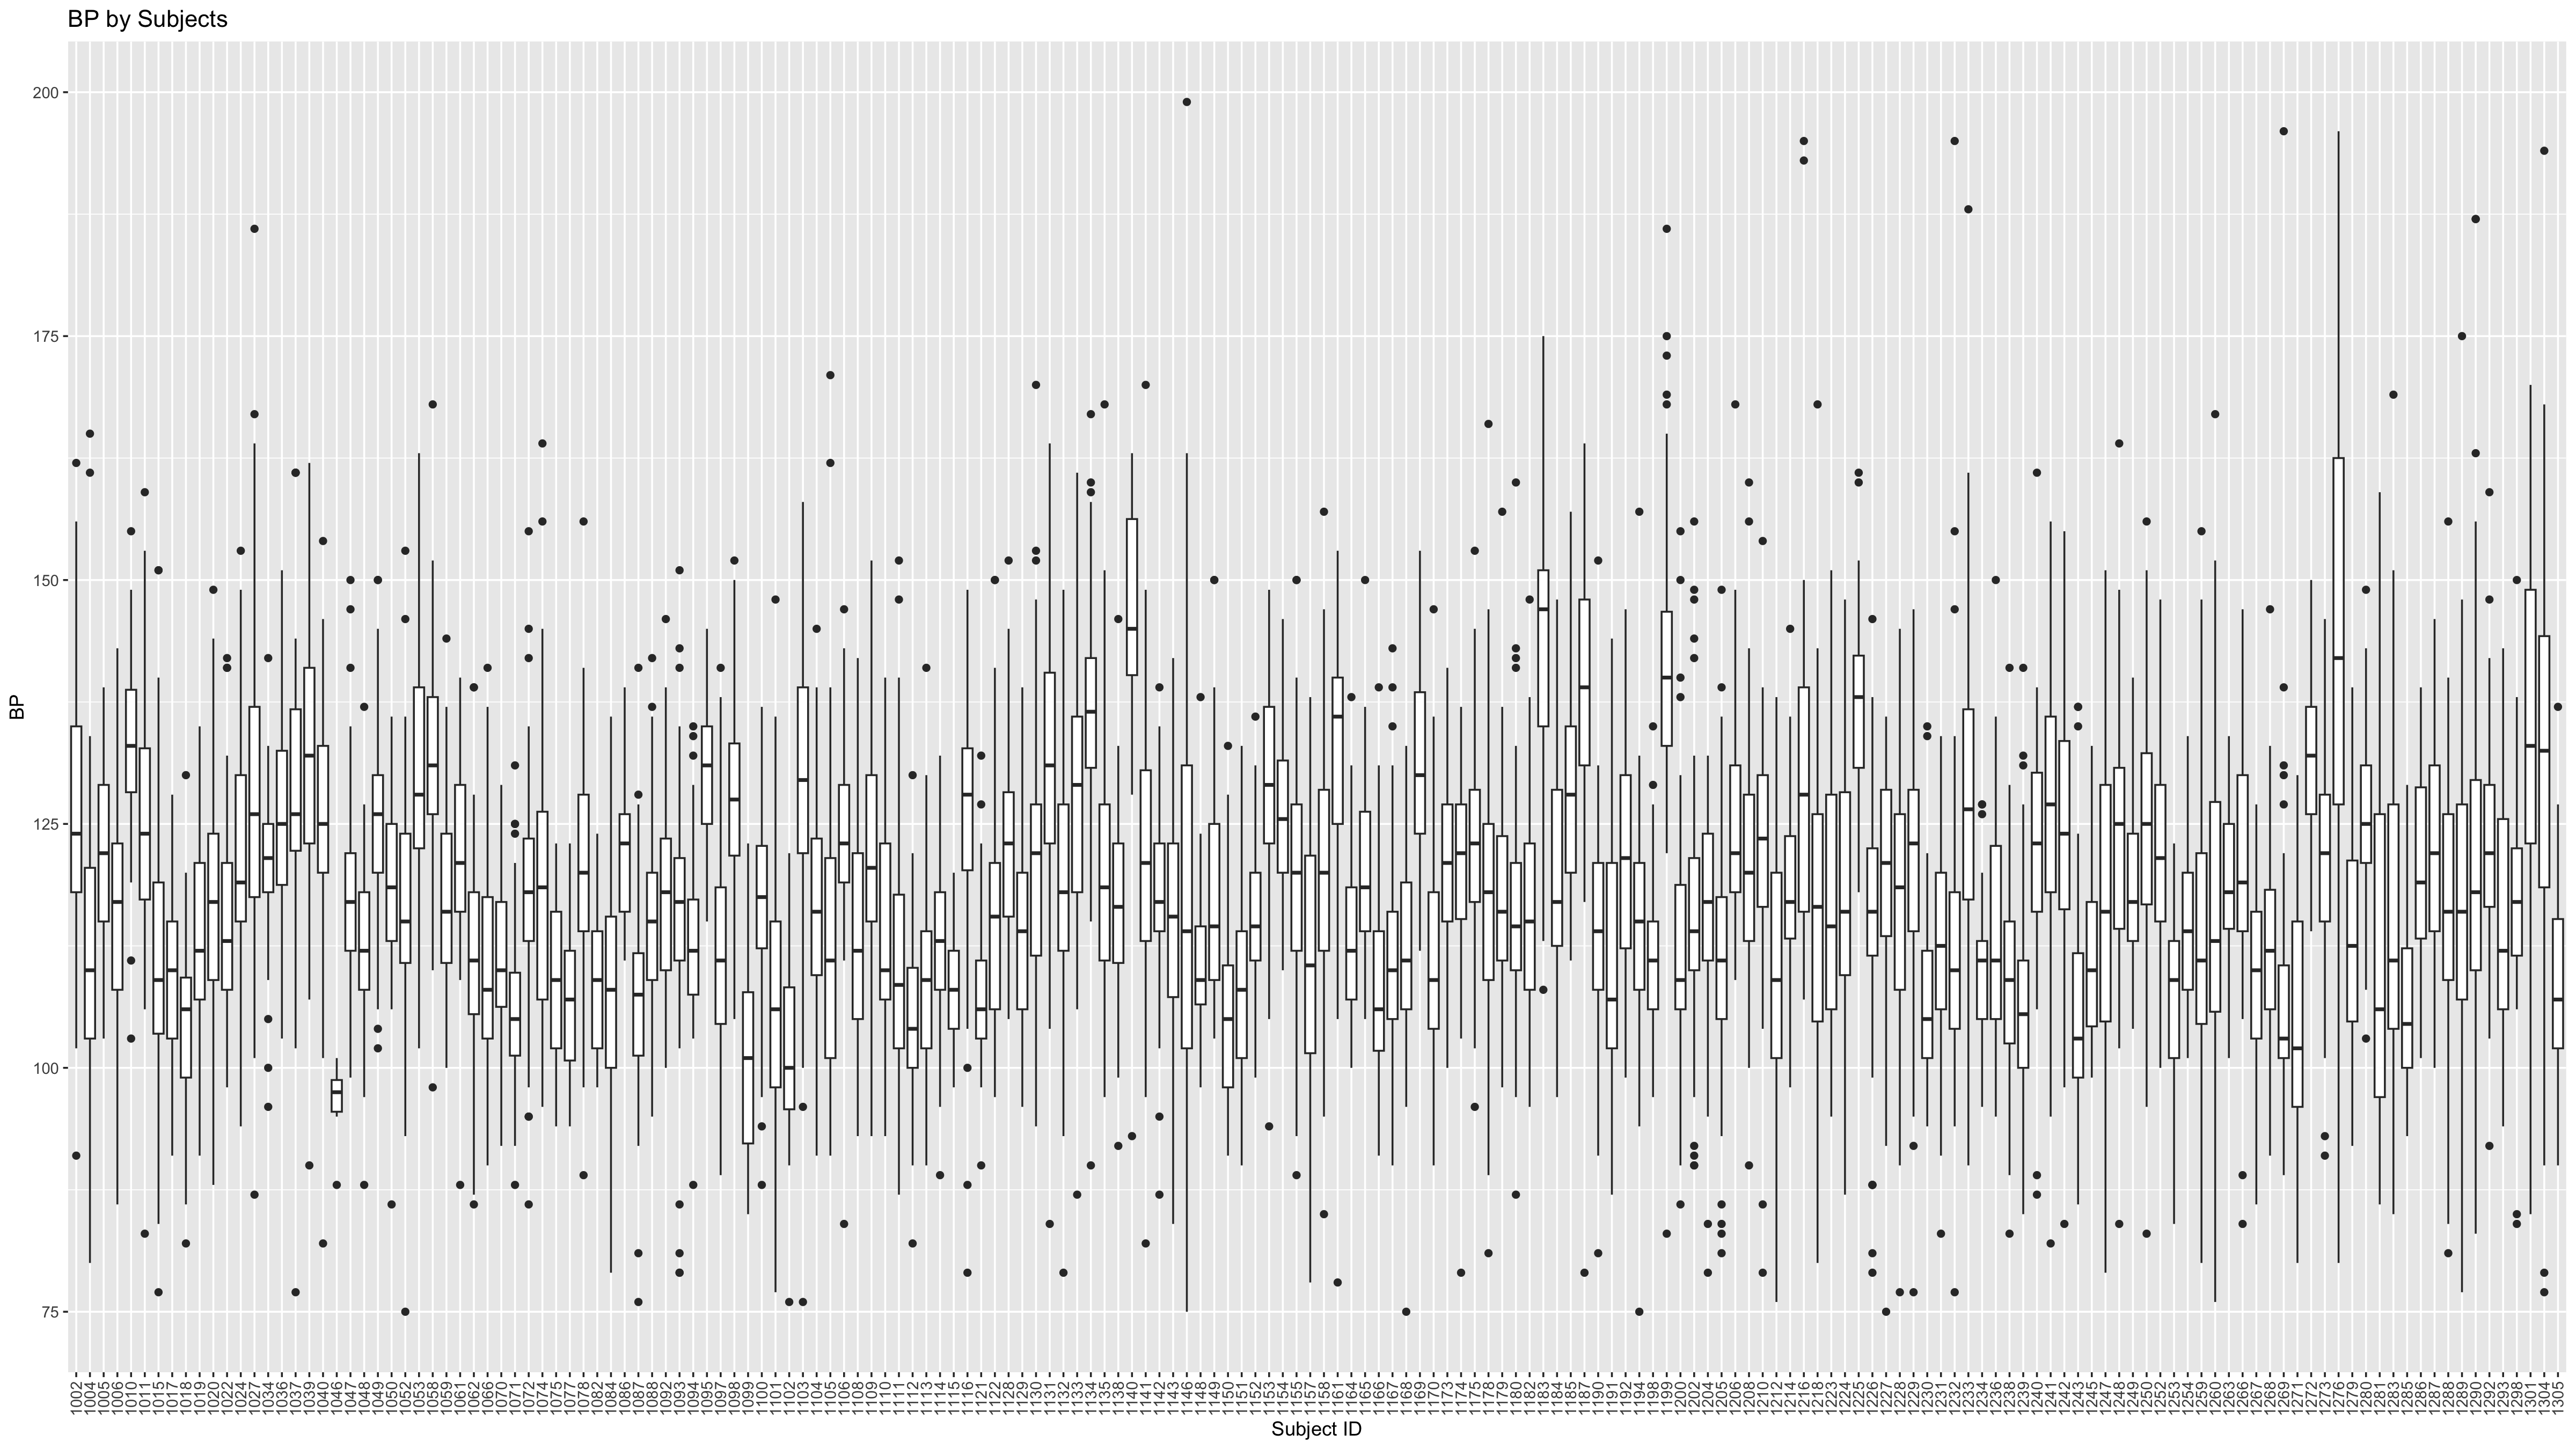
\includegraphics[width=\textwidth]{pics/bp by subjects.png}
    \caption{BP by Subjects}
    \label{fig: bp by subjects}
    \end{figure}

Since our data is ordered in time, one might be interested in answering how the participants' BP evolve over time. For sake of brevity, I show a random subsets of subjects and their BP readings over time in \Cref{fig: bp v time facet}. From this plot alone, not much could be deciphered; some trends (e.g., participant 1116) seem to decrease over time while others either slightly increase (e.g., participant 1267) or do not see much fluctuation overall. Indeed, when I fit separate linear smoothers for each participant, I see various different intercepts and slopes for each participant (see \Cref{fig: bp v time separate ls}). This suggests that a random effect for both the intercept and slope of time.

\begin{figure} 
\centering
\begin{subfigure}[b]{0.48\textwidth}
\centering
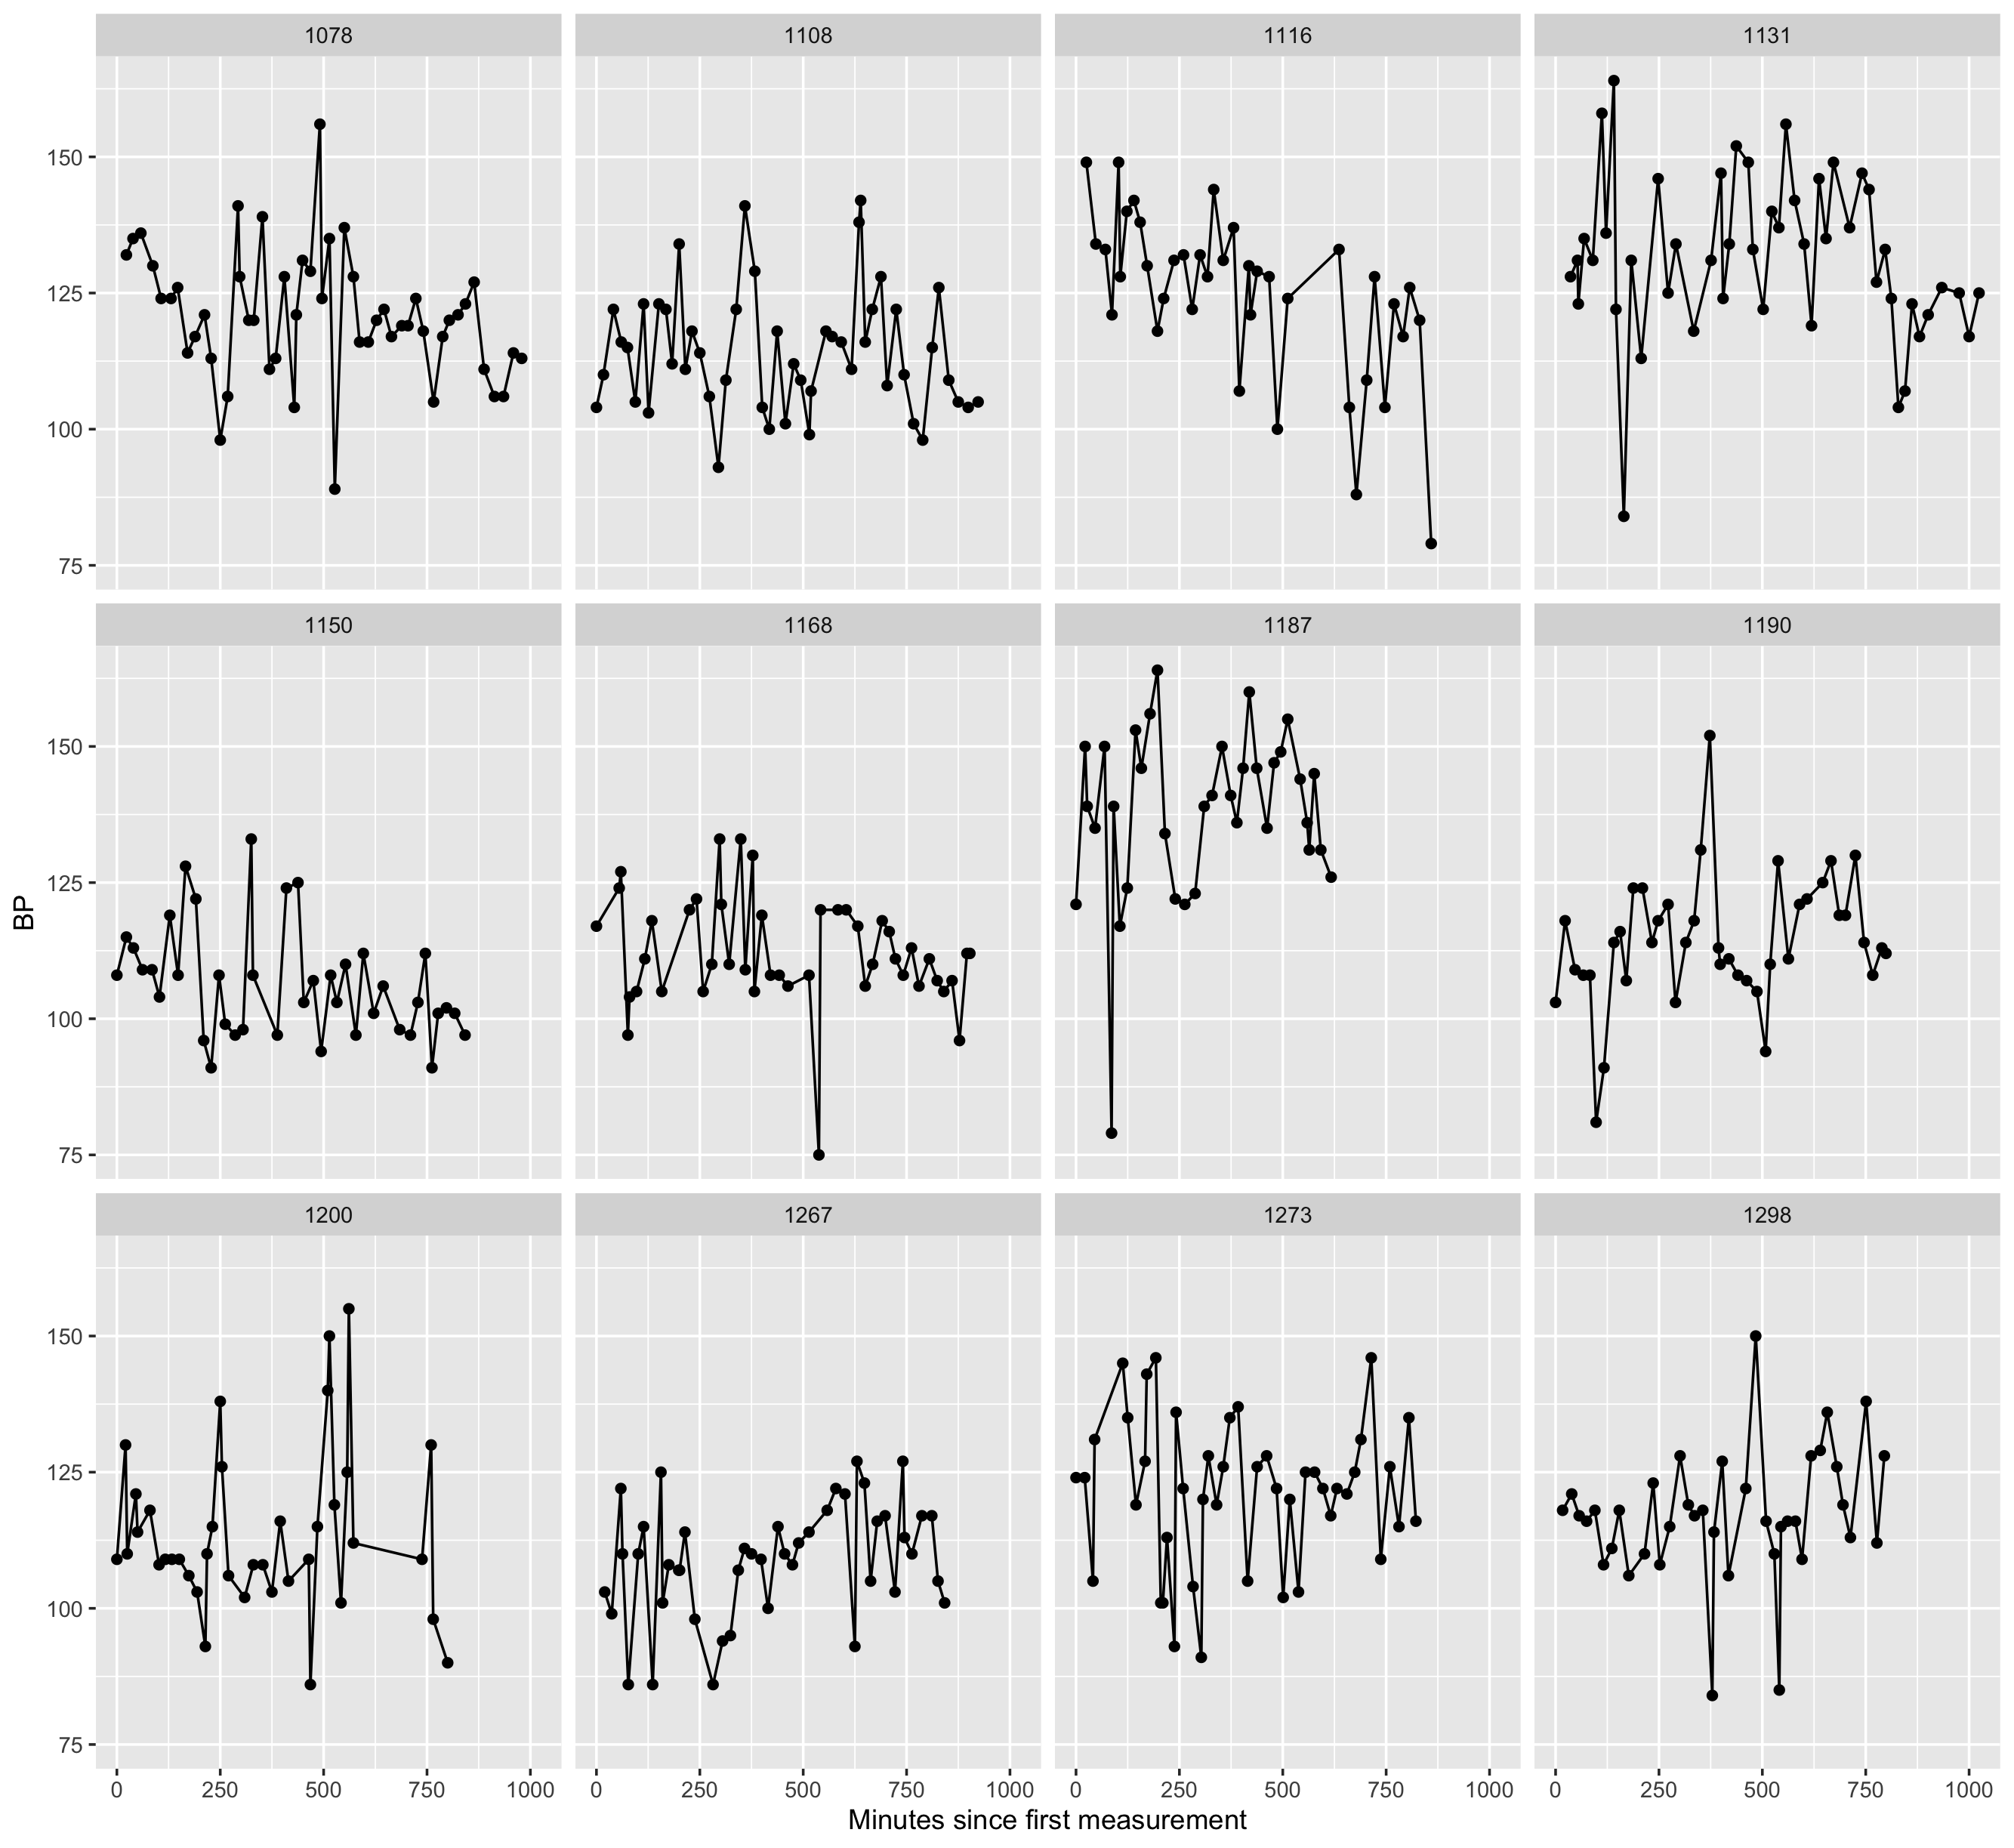
\includegraphics[width=\textwidth]{pics/bp v time by subj.png}
\caption[]%
{{\small BP vs. Time Passed by Subjects}}
\label{fig: bp v time facet}
\end{subfigure}
\hfill
\begin{subfigure}[b]{0.48\textwidth}
\centering
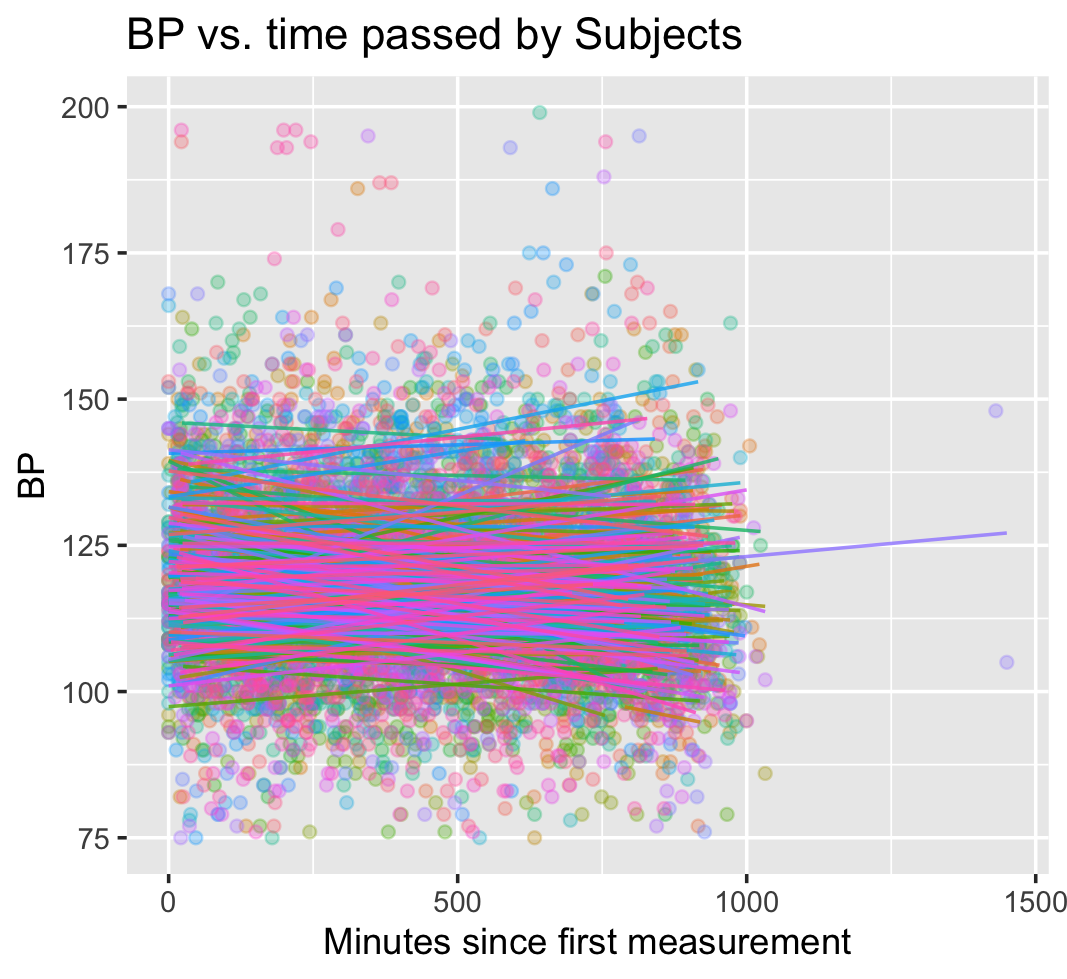
\includegraphics[width=\textwidth]{pics/BP v time LS.png}
\caption[]%
{{\small BP vs. Time Passed Separate Lines}}
\label{fig: bp v time separate ls}
\end{subfigure}
\caption[]
{\small BP vs. Minutes since first measurement}
\label{fig: bp v time}
\end{figure}

We perform similar analysis for other level 1 covariates (see \Cref{fig: bp v level1}). We see the most prominent effect in \texttt{Mood}, where the slopes and intercepts for each participant differs the most. They all show, to a certain extend, signs of varying slopes and intercepts, but I cannot definitely conclude anything at this point.

\begin{figure} 
    \centering
    \begin{subfigure}[b]{0.32\textwidth}
    \centering
    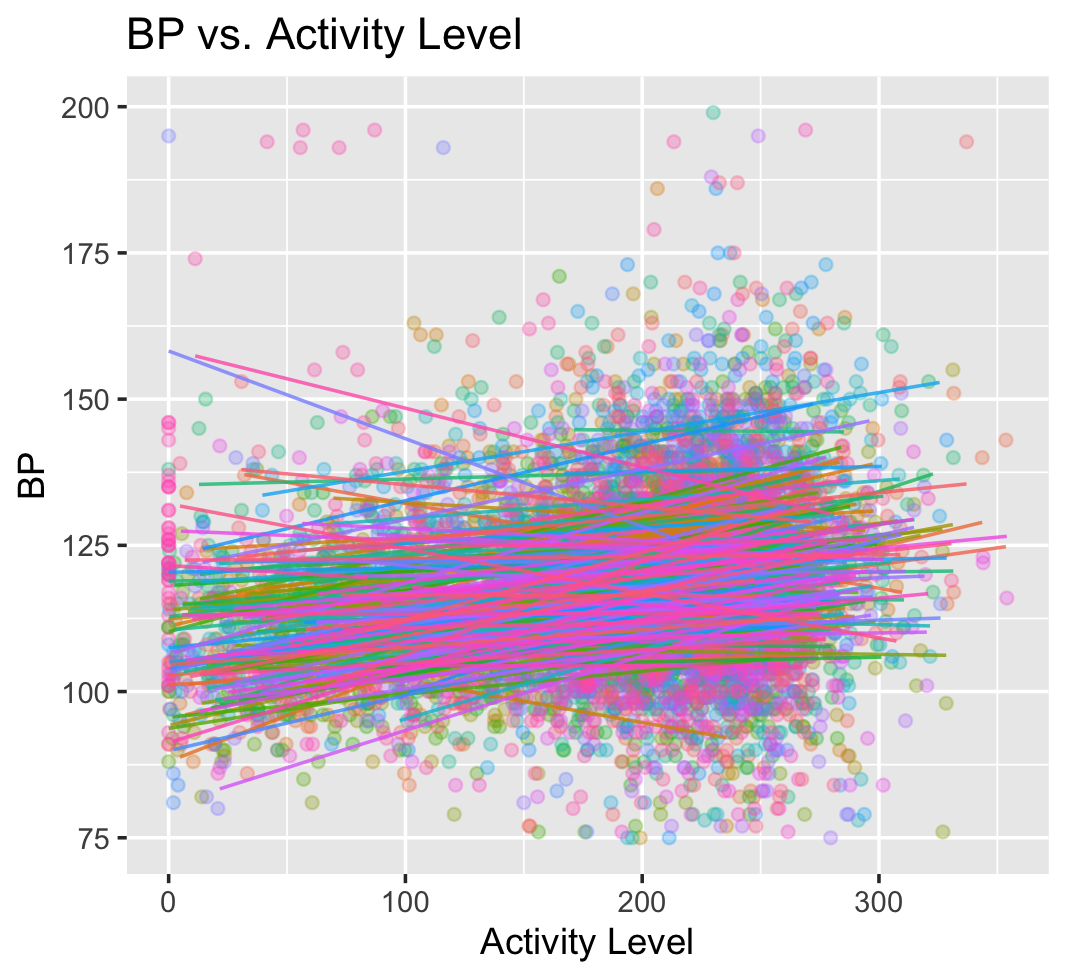
\includegraphics[width=\textwidth]{pics/bp v act.png}
    \caption[]%
    {{\small BP vs. Activity Level by Subjects}}
    \label{fig: bp v act}
    \end{subfigure}
    \hfill
    \begin{subfigure}[b]{0.32\textwidth}
    \centering
    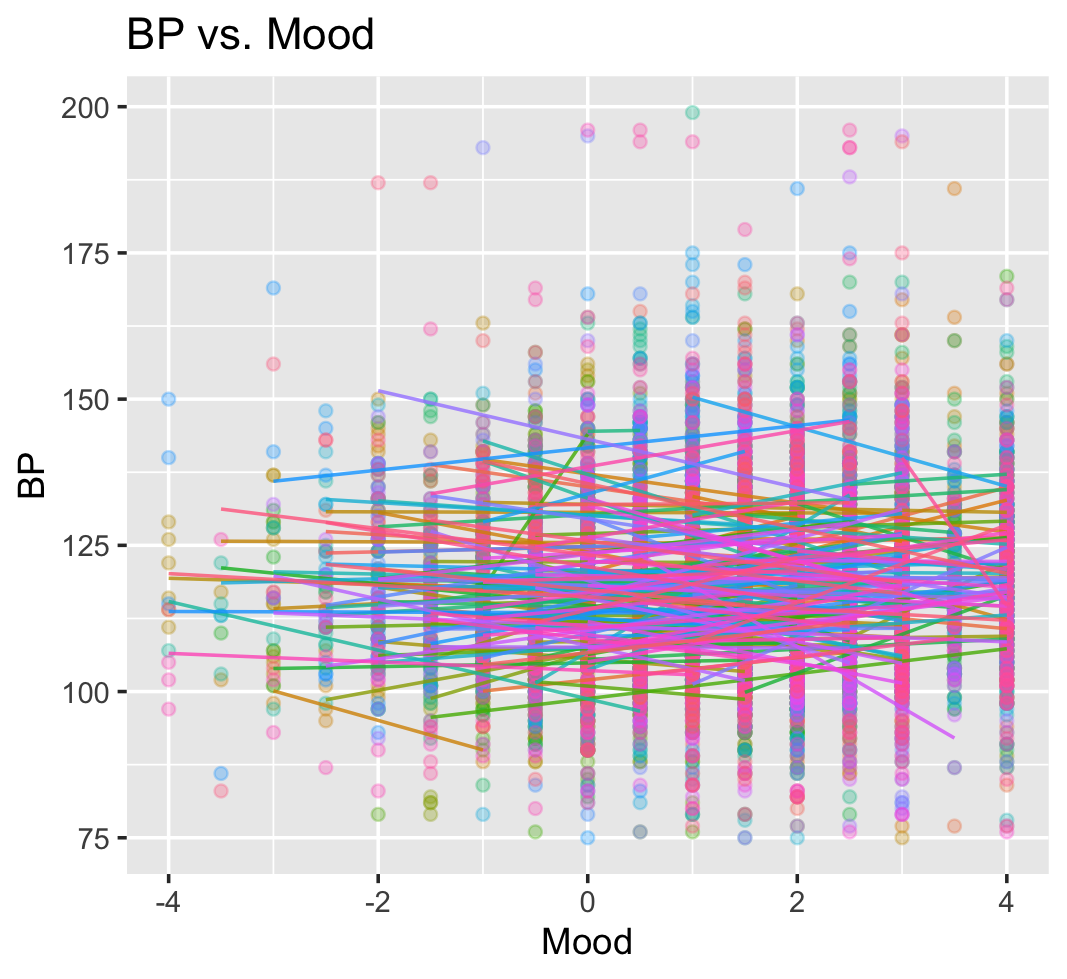
\includegraphics[width=\textwidth]{pics/bp v mood.png}
    \caption[]%
    {{\small BP vs. Mood Ratings by Subjects}}
    \label{fig: bp v mood}
    \end{subfigure}
    \hfill
    \begin{subfigure}[b]{0.32\textwidth}
    \centering
    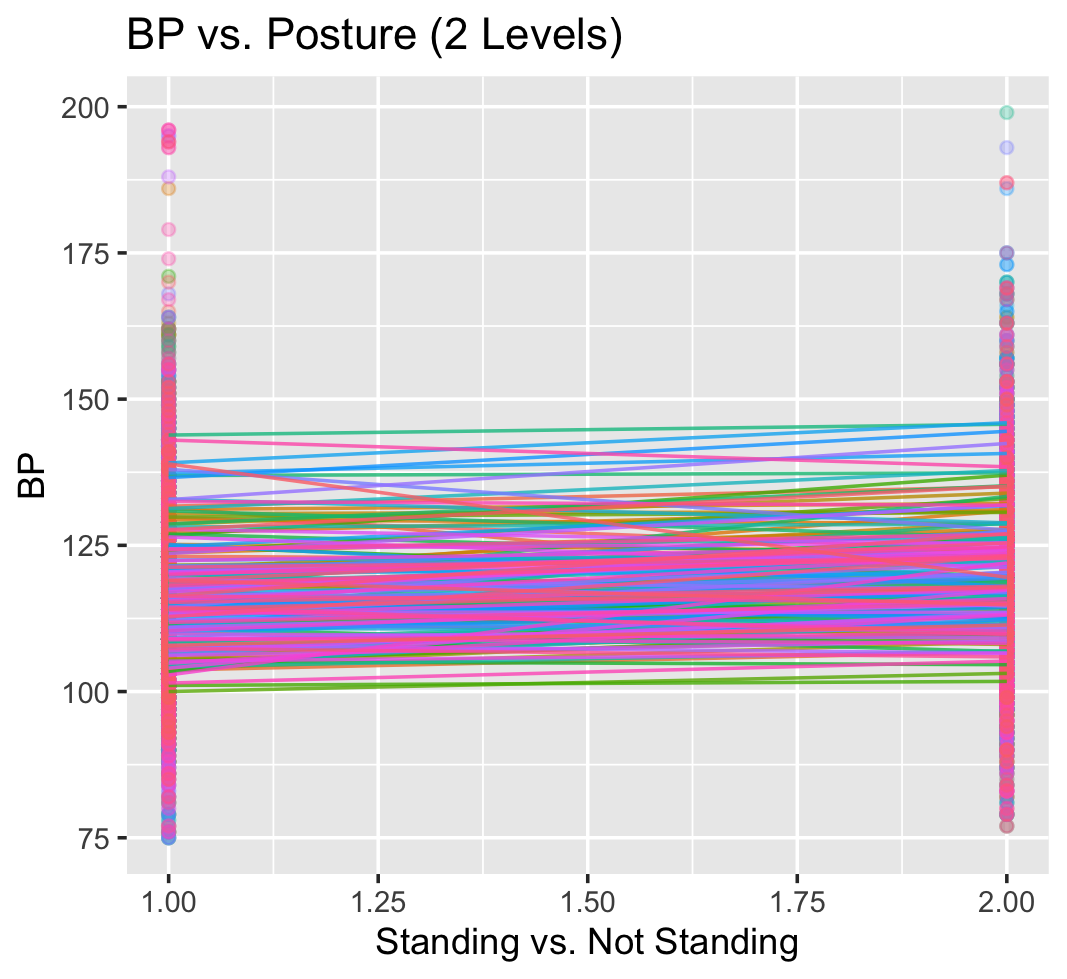
\includegraphics[width=\textwidth]{pics/bp v stand.png}
    \caption[]%
    {{\small BP vs. Posture (Standing) by Subjects}}
    \label{fig: bp v stand}
    \end{subfigure}
    \caption[]
    {\small BP vs. Level 1}
    \label{fig: bp v level1}
    \end{figure}

\subsection{Level 2 Covariates}\label{sec: lv2}

We then want to understand the distributions of our level two covairates before we look at any interactions between the two levels. Because our level 2 covariates contains the same measurement over time (whereas our primary response \texttt{BP} is level 1 and hence time-dependent), we will compare the level 2 covariates with the \emph{average} \texttt{BP} of a given participant. 

From \Cref{fig: bp v phase}, we do not see that being on a different menstural phase impacts the participants' average \texttt{BP} much at all, suggesting that we likely do not need to control for \texttt{Phase} as a level 2 predictor. We see that in a workday, as opposed to a non-workday, the average \texttt{BP} of the participants appears to have a higher mean (see \Cref{fig: bp v day}). 

Similarly for family history; having at least one parent with hypertension bumps the participants' average \texttt{BP} by a marginal amount (\Cref{fig: bp v fh}). This suggest that we might want to look into having \texttt{Day} and \texttt{FH} in our model as control or predictors; we will return to their interaction with level 1 predictors in the next section. 

Lastly, it is unclear how age impacts average \texttt{BP}, since \Cref{fig: bp v age} shows that the effect of age varies significantly (though a smoother line shows slight positive increase as age increases). We will test this formally in \Cref{sec: model selection}.

\begin{figure} 
    \centering
    \begin{subfigure}{0.48\textwidth}
        \centering
        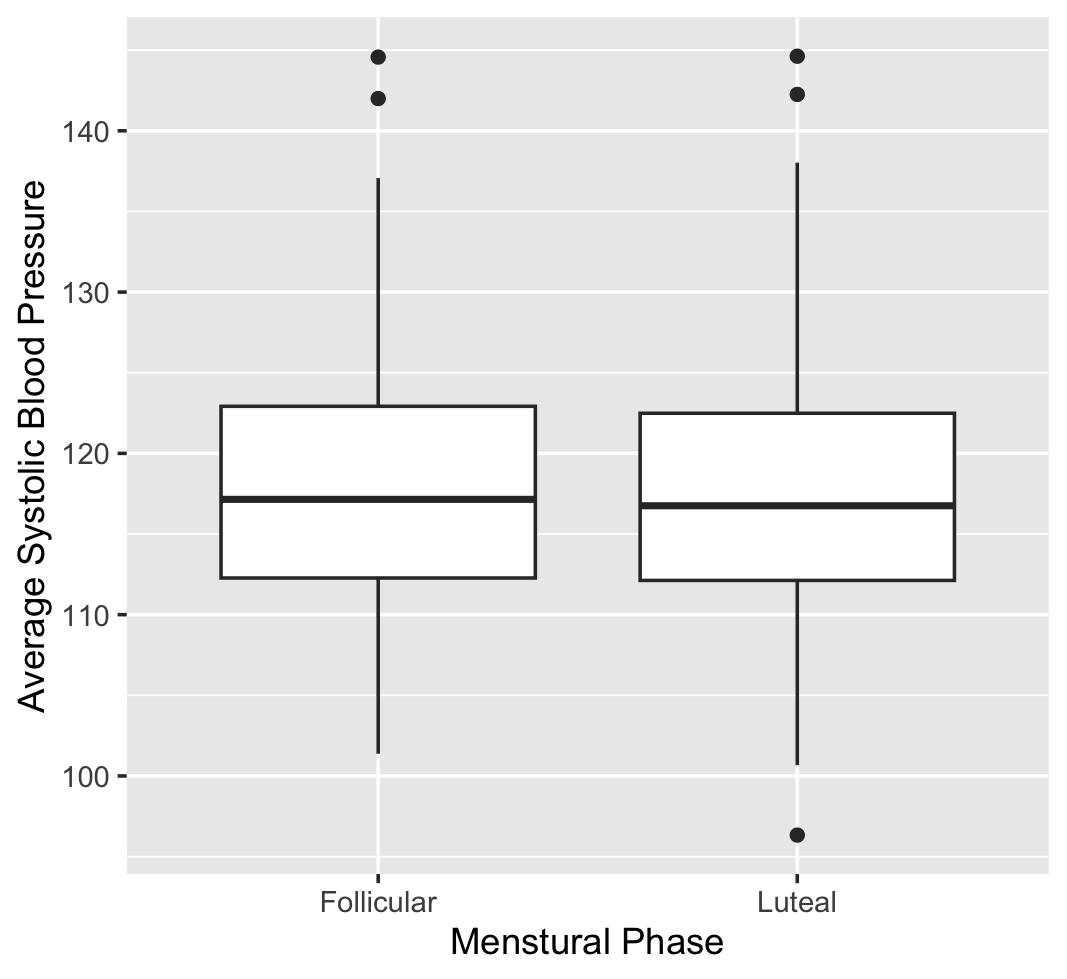
\includegraphics[width=\textwidth]{pics/bp v phase.png}
        \caption{{\small Avg BP vs. Menstrual Phase}}
        \label{fig: bp v phase}
    \end{subfigure}
    \hfill
    \begin{subfigure}{0.48\textwidth}
        \centering
        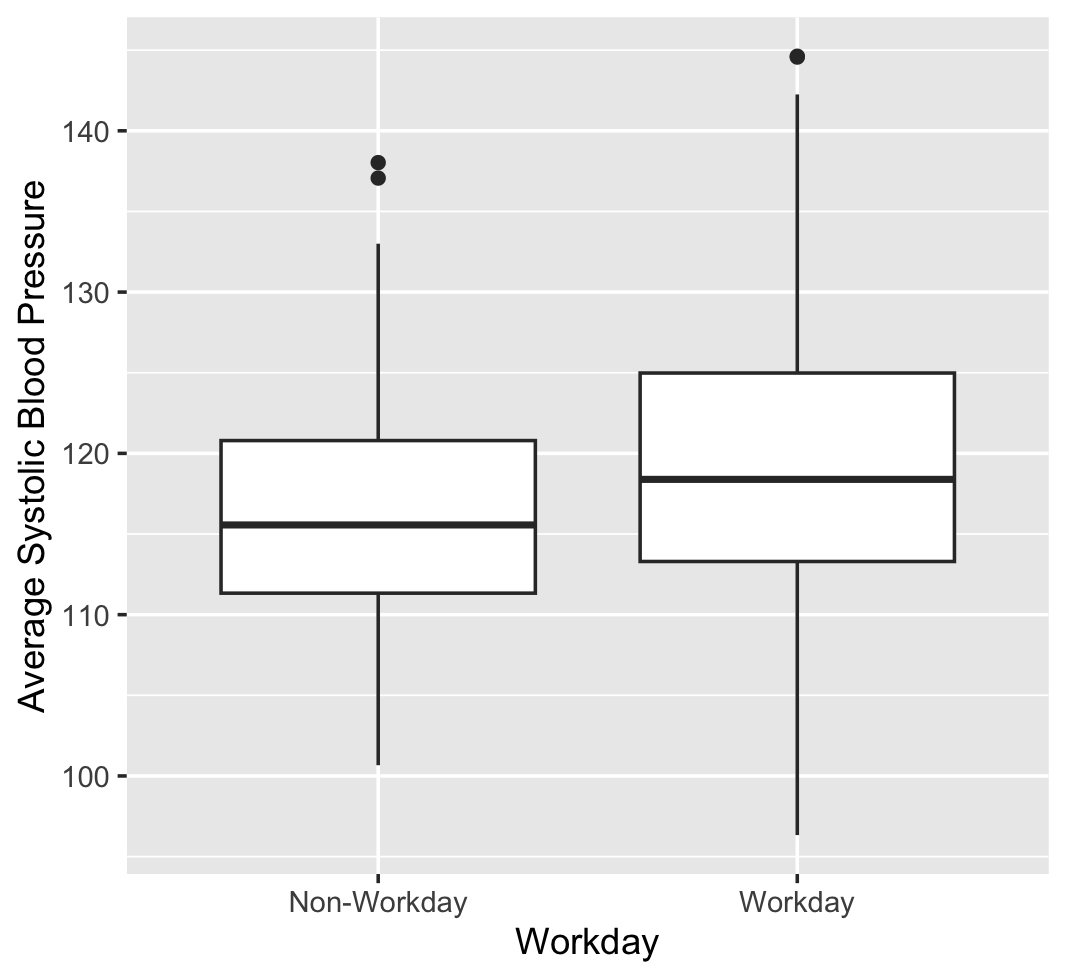
\includegraphics[width=\textwidth]{pics/bp v day.png}
        \caption{{\small Avg BP vs. Workday}}
        \label{fig: bp v day}
    \end{subfigure}
    \caption{{\small Average BP vs. Level 2 Covariates}}
    \label{fig: bp v level2}
\end{figure}

\begin{figure}  \ContinuedFloat
    \centering
    \begin{subfigure}{0.48\textwidth}
        \centering
        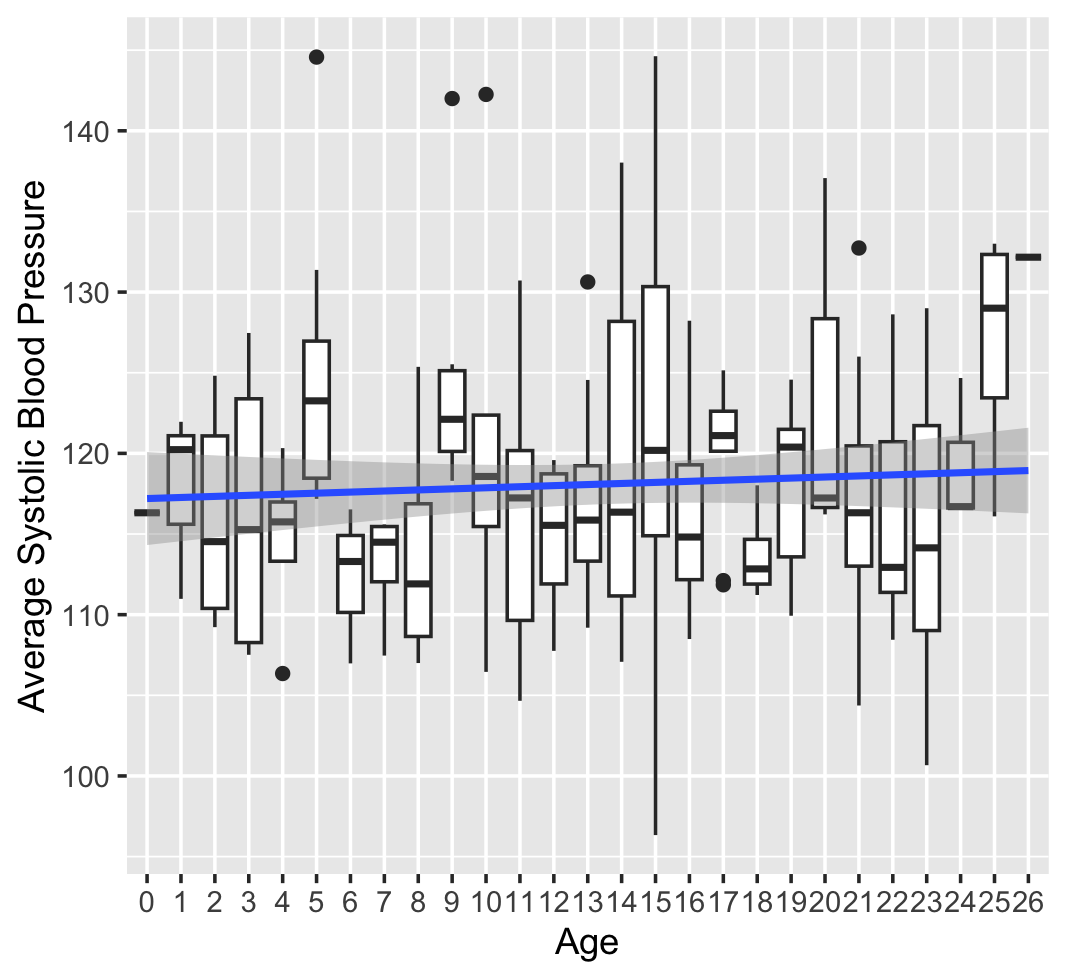
\includegraphics[width=\textwidth]{pics/bp v age.png}
        \caption{{\small Avg BP vs. Age}}
        \label{fig: bp v age}
    \end{subfigure}
    \hfill
    \begin{subfigure}{0.48\textwidth}
        \centering
        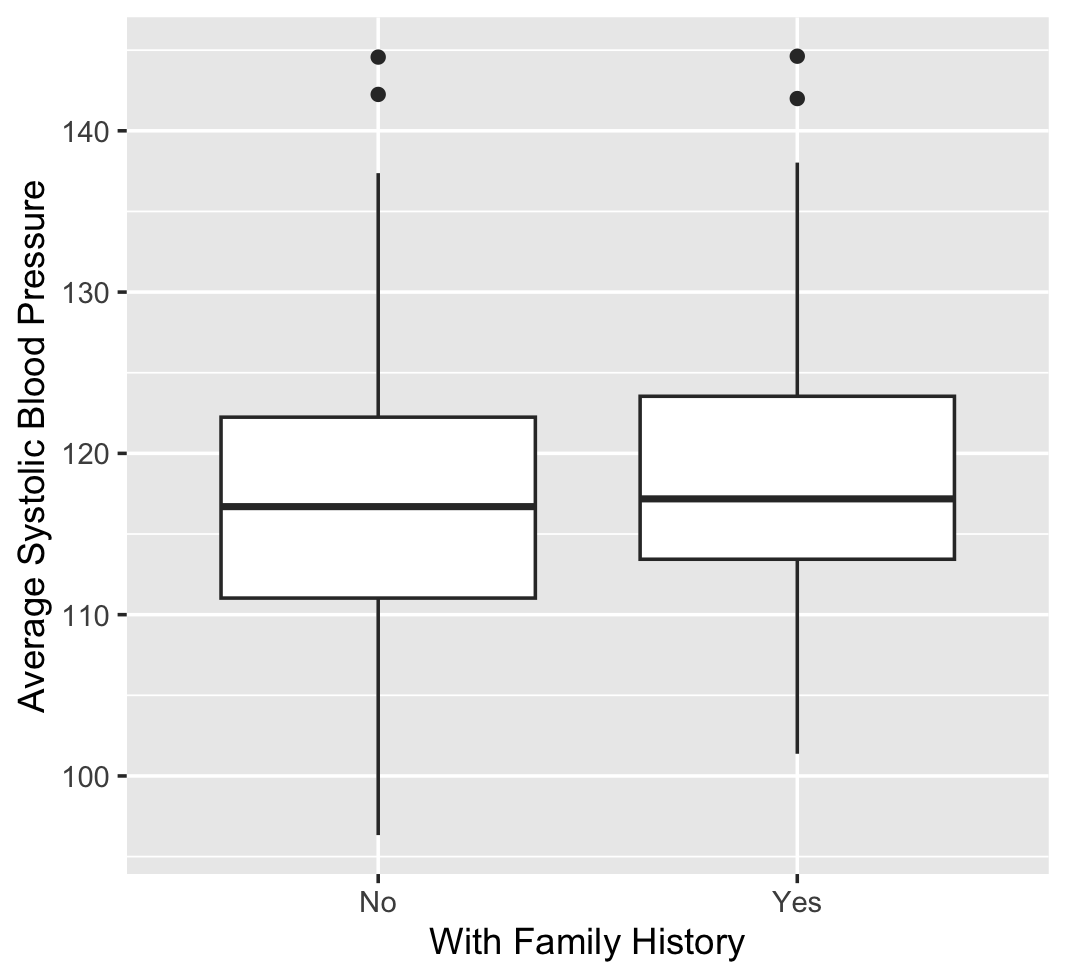
\includegraphics[width=\textwidth]{pics/bp v fh.png}
        \caption{{\small Avg BP vs. Family History}}
        \label{fig: bp v fh}
    \end{subfigure}
    \caption{{\small Average BP vs. Level 2 Covariates}}
    \label{fig: bp v level2 2}
\end{figure}

\subsection{Level 1 by Level 2 Covariates}\label{sec: lv1 x lv2}

Next we investigate whether our level 1 covariates depend, in any way, on our level 2 covariates. There are several ways one could explore this.\footnote{Additional visualizations are shown in \autoref{sec: add visuals}.} In \Cref{sec: lv2}, we suspect that \texttt{BP} depends on \texttt{Workday} and \texttt{FH}. Instead of showing the average \texttt{BP}, we can also show simply the level 1 responses, faceted by workday and family history (see \Cref{fig: bp by day and fh}).

\begin{figure} 
\centering
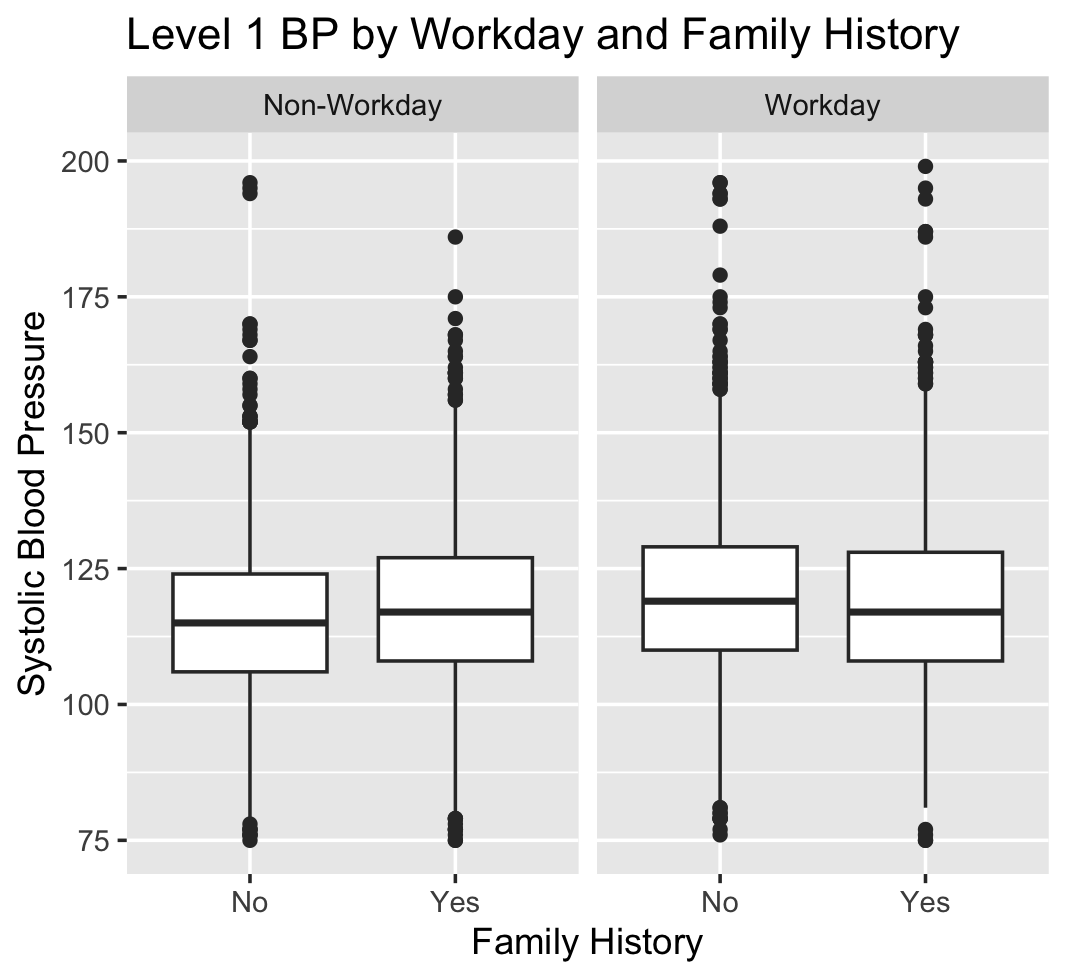
\includegraphics[width=0.4\textwidth]{pics/bp by day and fh.png}
\caption{Level 1 BP by Workday and Family History}
\label{fig: bp by day and fh}
\end{figure}

To better understand the interaction between level 2 covairates and the level 1 covairates, however, it is most clear to explore with spaghetti plots or separate LS models to see the difference in intercepts and slopes. We first explore with spaghetti plots. From \Cref{fig: bp v level1 and day2} alone, it is hard to say anything conclusive about whether one of the level one covariates depend on \texttt{Workday}; there all seem to be marginal difference in intercepts, but slopes seem largely similar. \Cref{fig: bp v level1 and fh2} likewise shows inconclusive results in terms of \texttt{Family History} (though there appears to be some difference in slopes in Mood by \texttt{FH}). We proceed to analyze separate MLR models containing level 1 variables for each participant. This also allows us to better understand the continuous variable \texttt{Age24}. 

\begin{figure} 
    \centering
    \begin{subfigure}{0.48\textwidth}
        \centering
        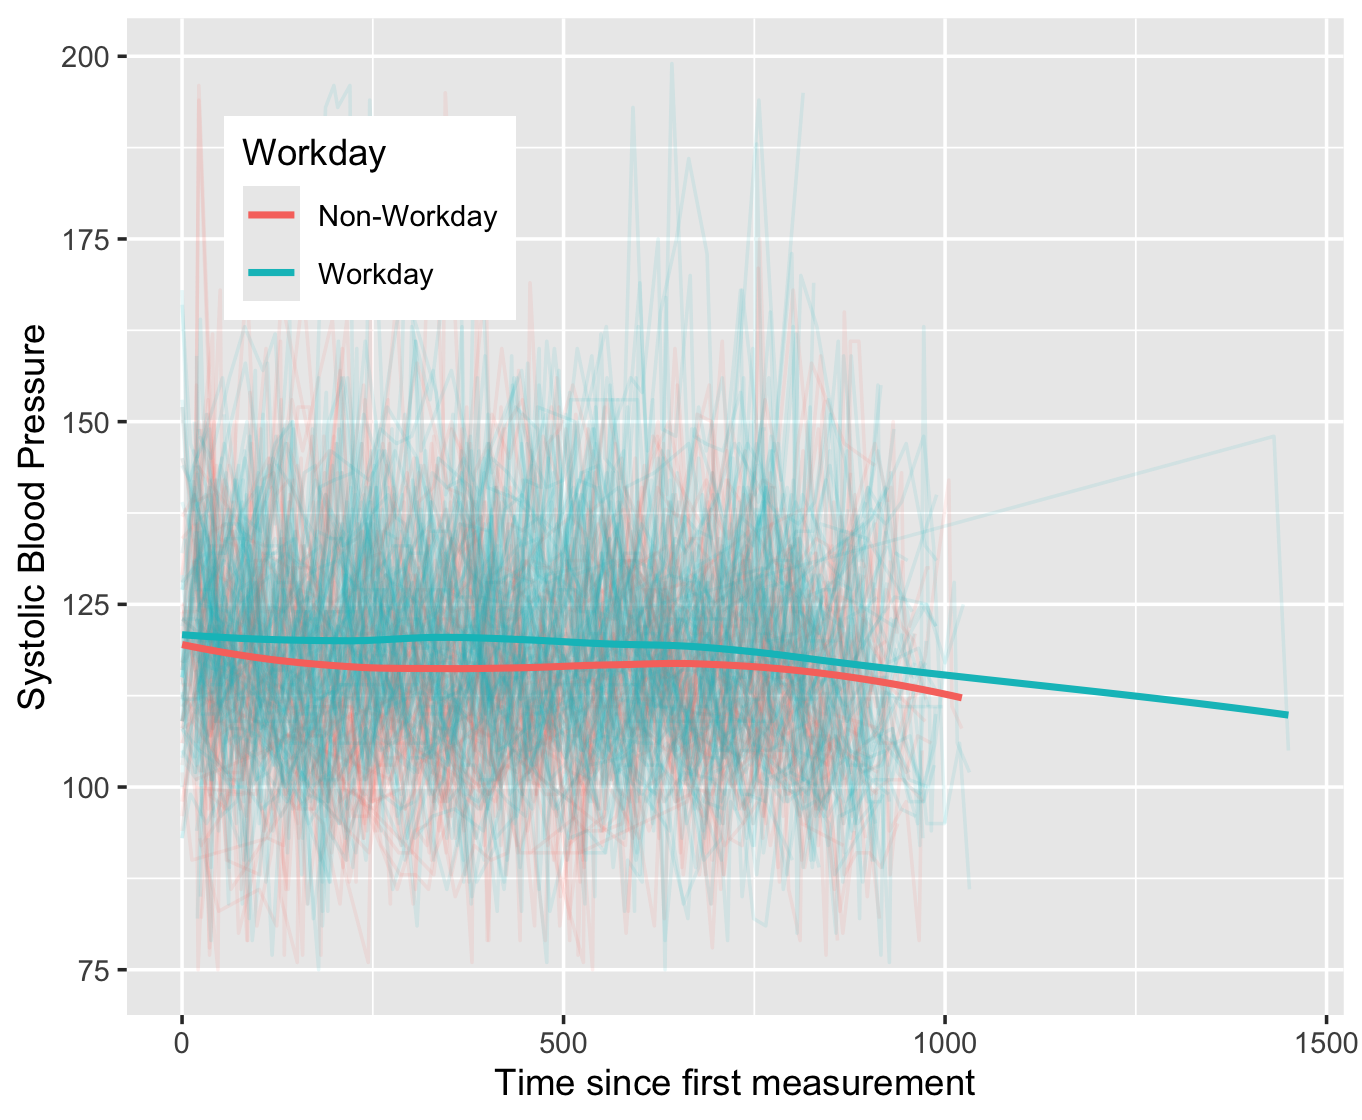
\includegraphics[width=\textwidth]{pics/bp v time and day.png}
        \caption{{\small L1 BP vs. Time by Workday}}
        \label{fig: bp v time and day}
    \end{subfigure}
    \hfill
    \begin{subfigure}{0.48\textwidth}
        \centering
        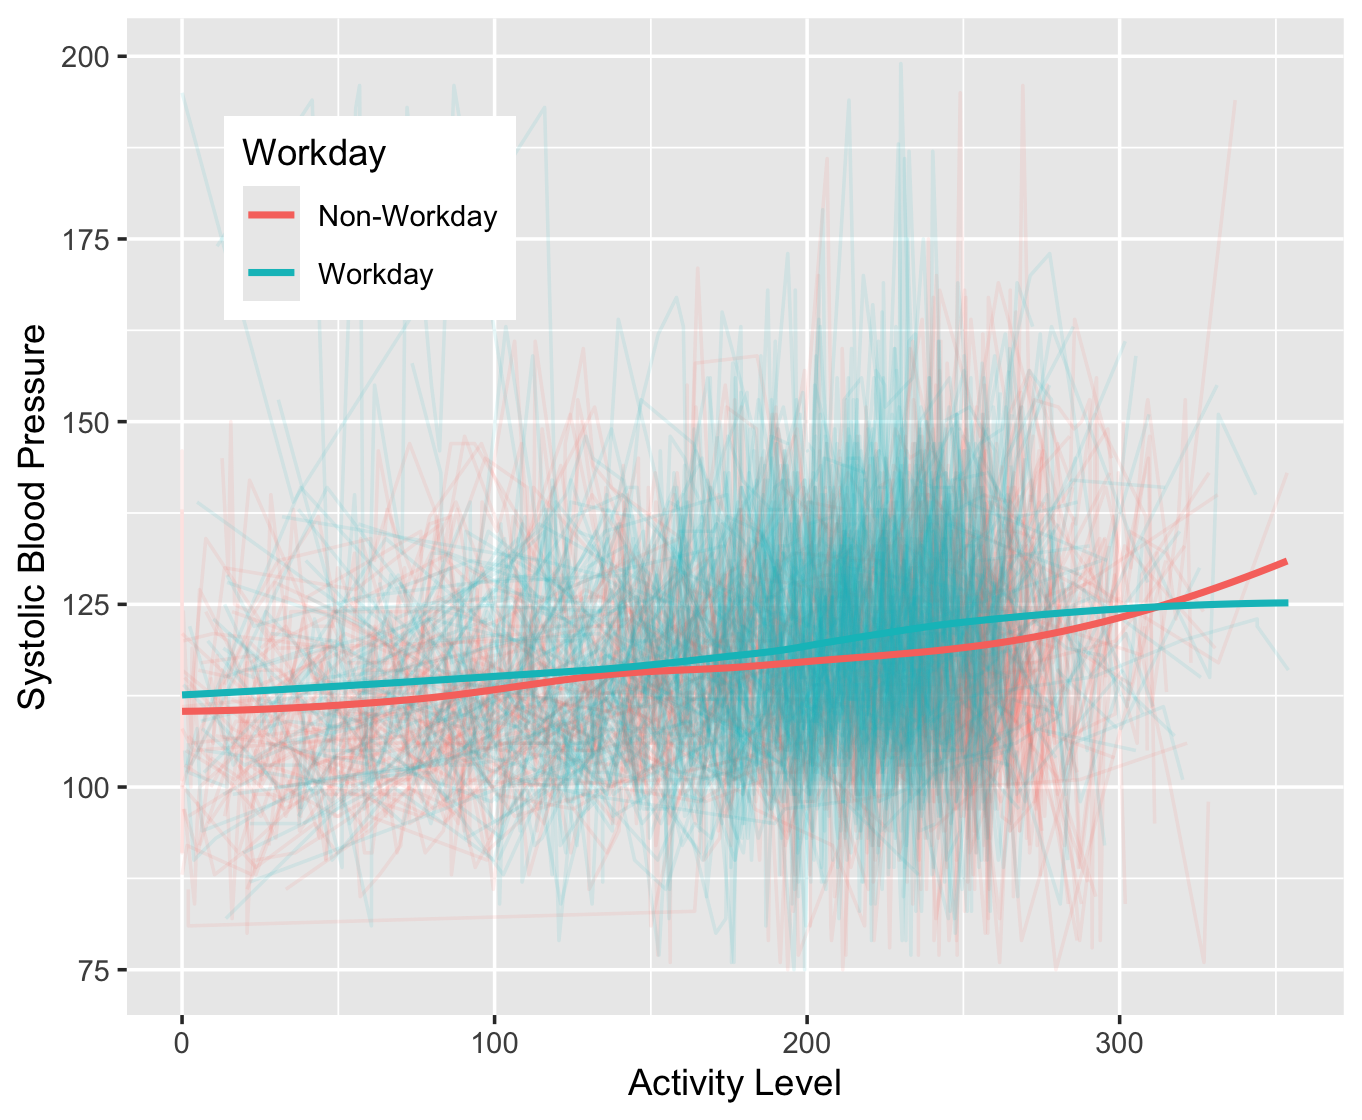
\includegraphics[width=\textwidth]{pics/bp v act and day.png}
        \caption{{\small L1 BP vs. Activity by Workday}}
        \label{fig: bp v act and day}
    \end{subfigure}
    \vskip\baselineskip
%     % \caption{{\small L1 BP vs. Level 1 Covariates by Workday}}
%     % \label{fig: bp v level1 and day}
% \end{figure}

% \begin{figure}  \ContinuedFloat
%     \centering
    \begin{subfigure}{0.48\textwidth}
        \centering
        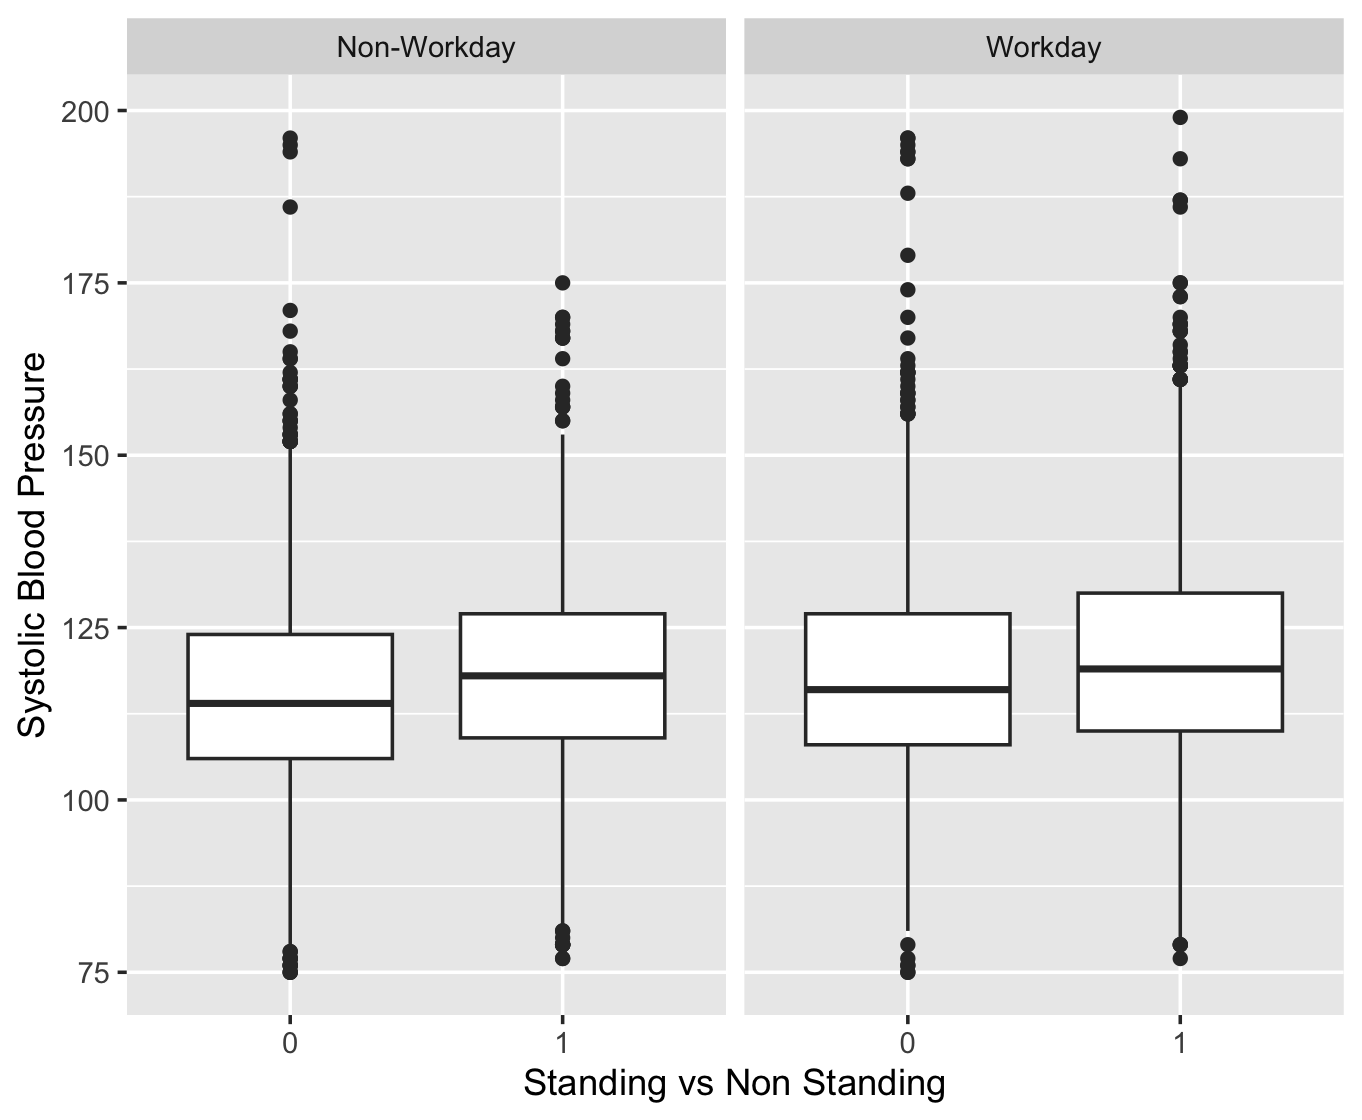
\includegraphics[width=\textwidth]{pics/bp v stand and day.png}
        \caption{{\small L1 BP vs. Standing by Workday}}
        \label{fig: bp v stand and day}
    \end{subfigure}
    \hfill
    \begin{subfigure}{0.48\textwidth}
        \centering
        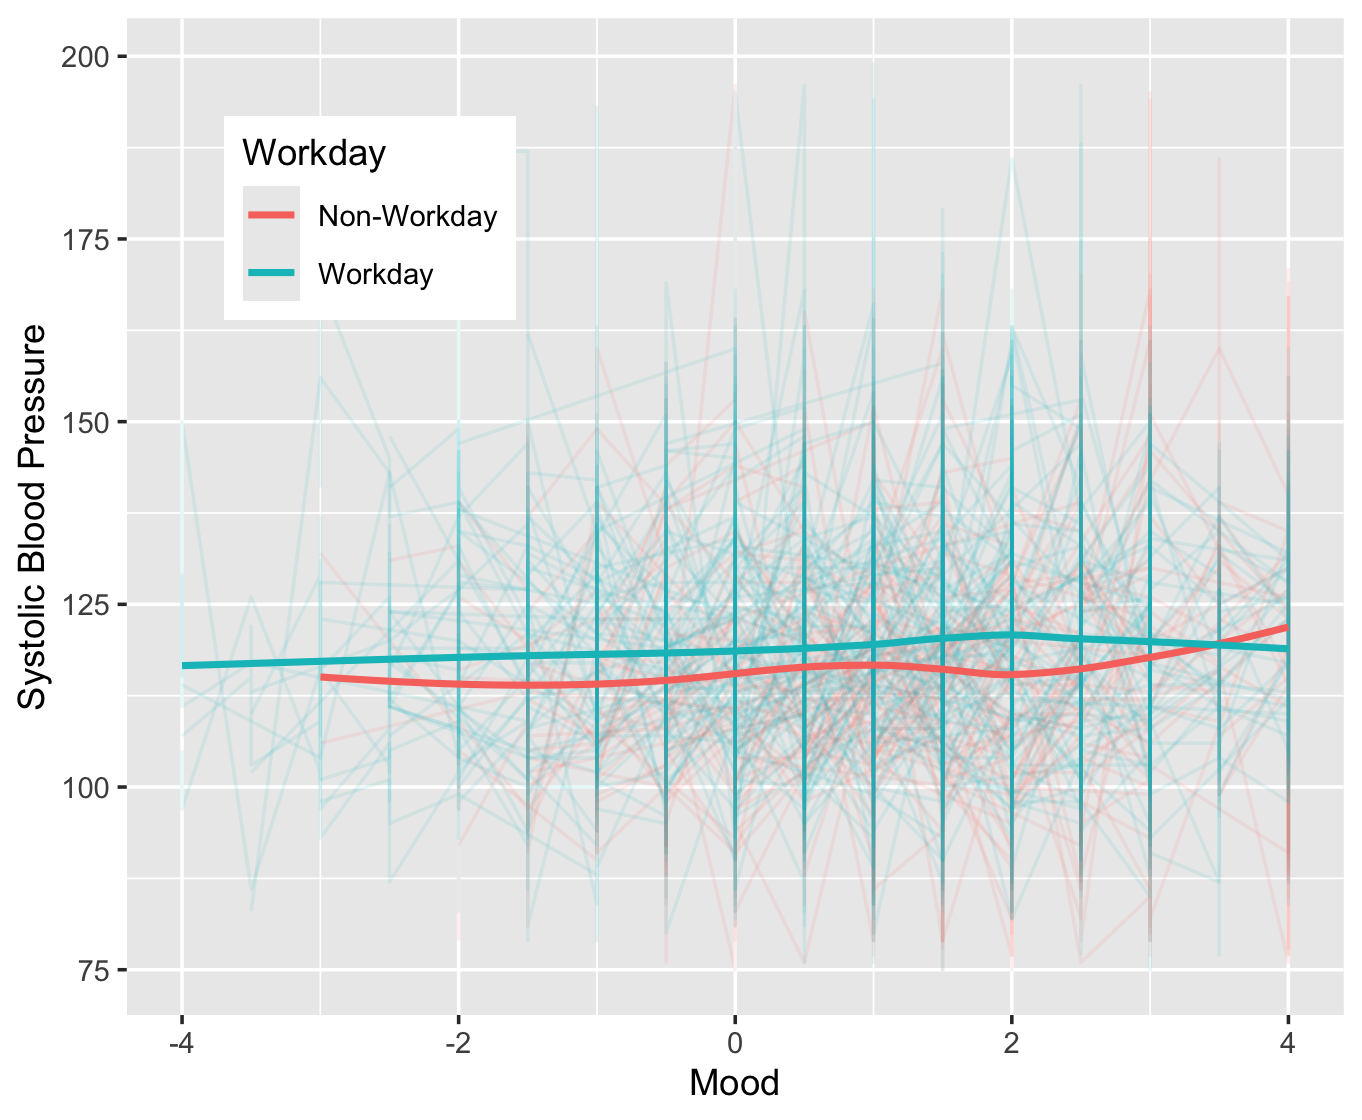
\includegraphics[width=\textwidth]{pics/bp v mood and day.png}
        \caption{{\small L1 BP vs. Mood by Workday}}
        \label{fig: bp v mood and day}
    \end{subfigure}
    \caption{{\small L1 BP vs. Level 1 Covariates by Workday}}
    \label{fig: bp v level1 and day2}
\end{figure}

\begin{figure} 
    \centering
    \begin{subfigure}{0.48\textwidth}
        \centering
        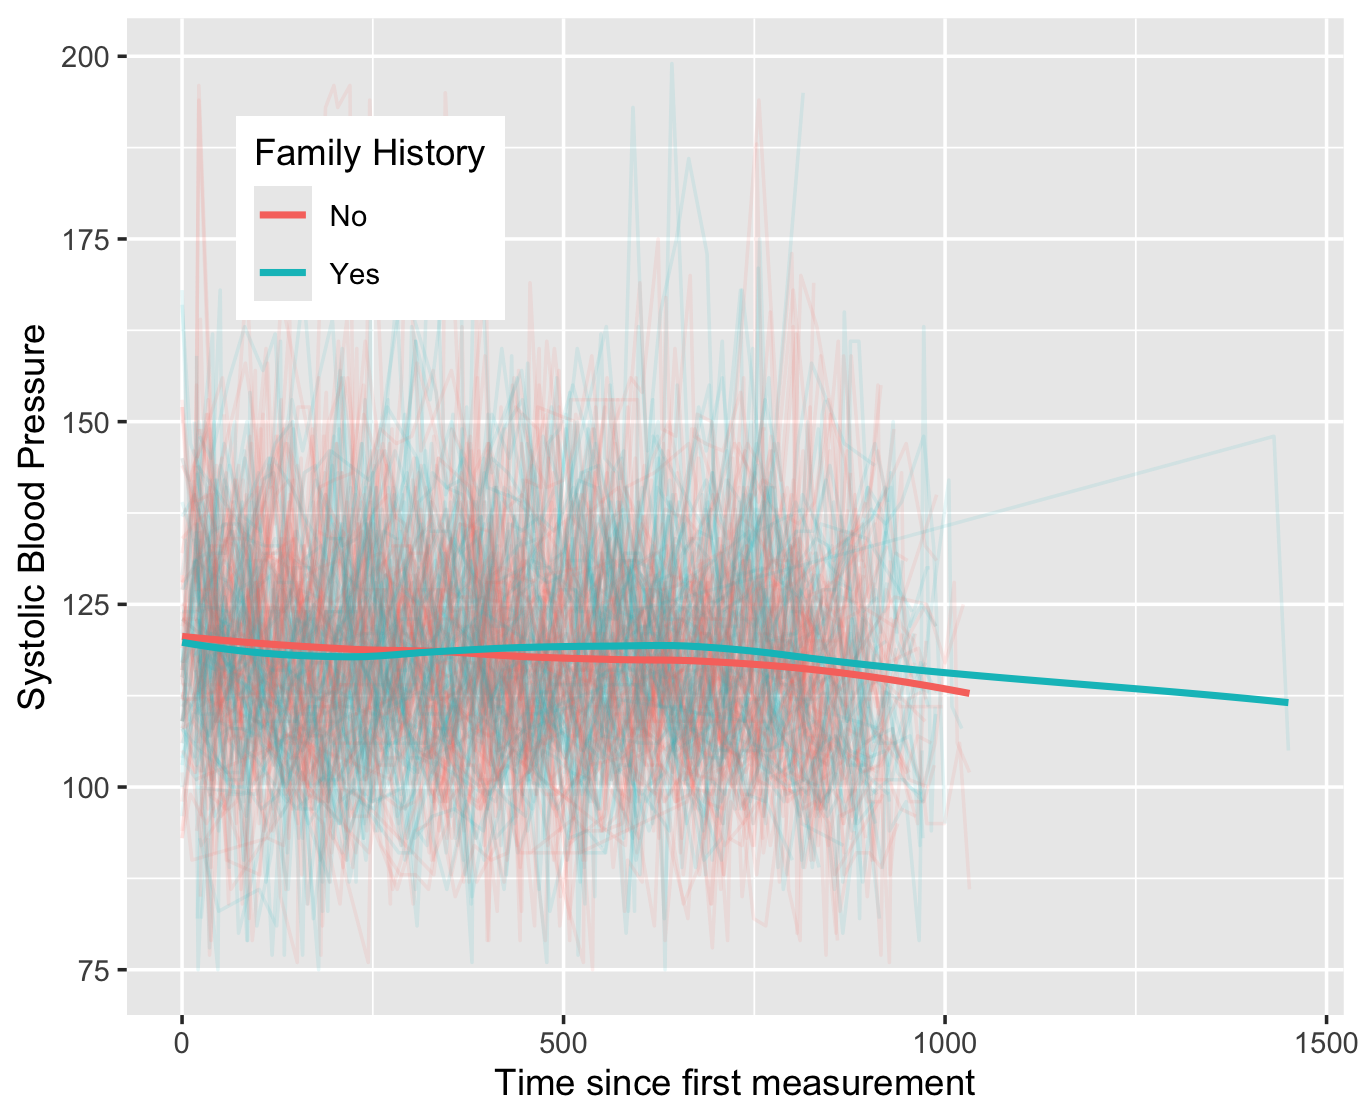
\includegraphics[width=\textwidth]{pics/bp v time and fh.png}
        \caption{{\small L1 BP vs. Time by Family History}}
        \label{fig: bp v time and fh}
    \end{subfigure}
    \hfill
    \begin{subfigure}{0.48\textwidth}
        \centering
        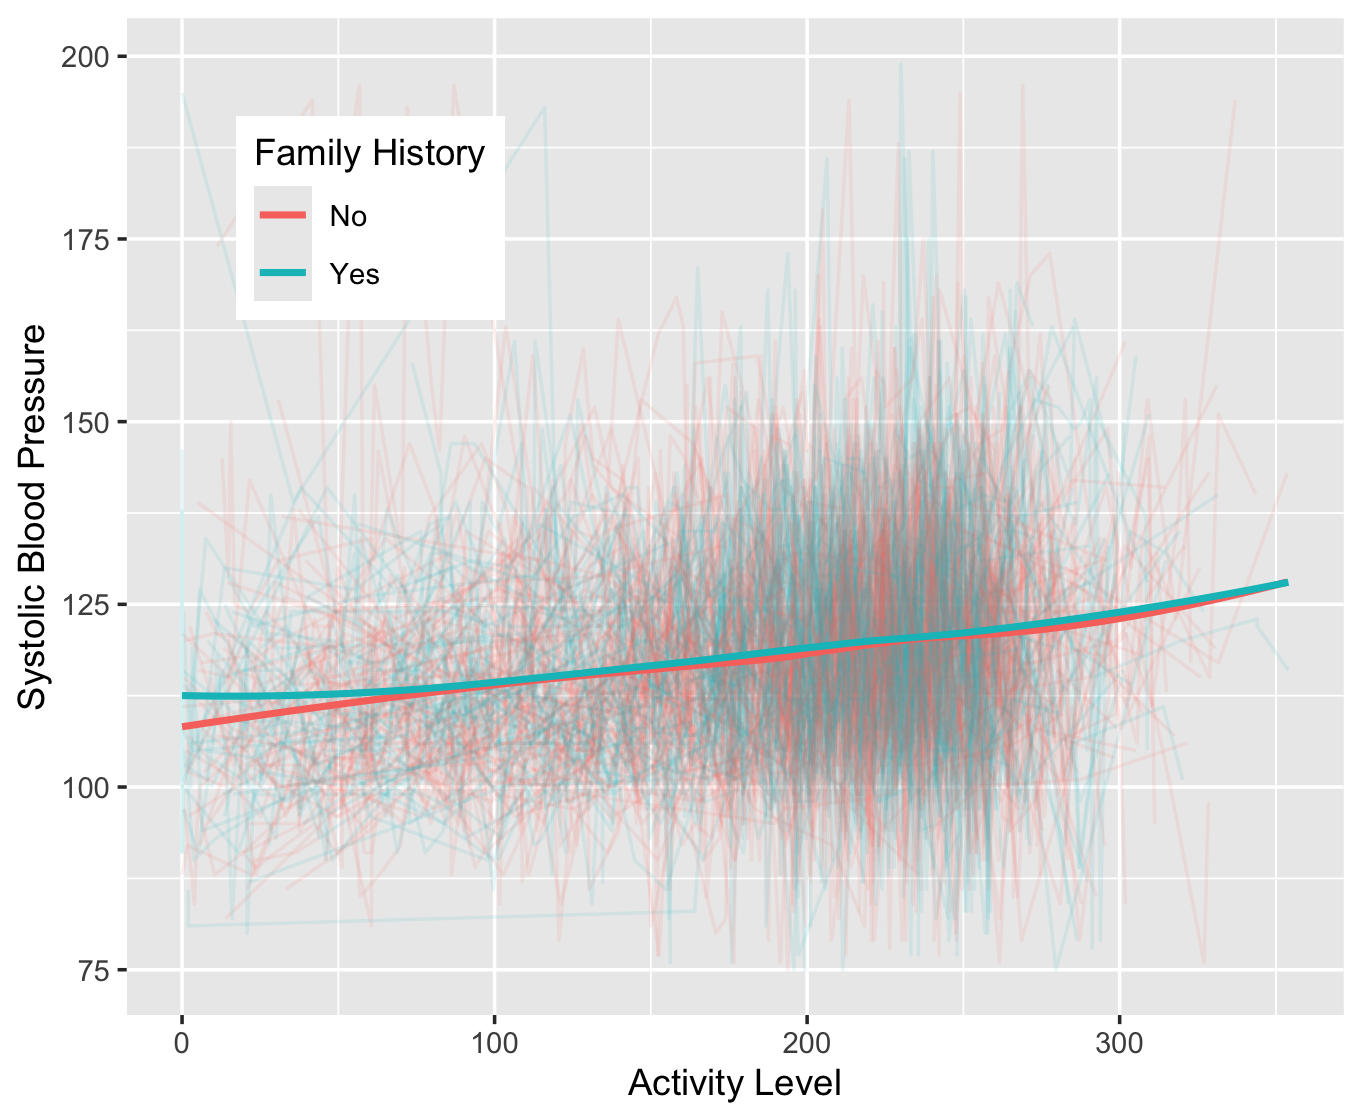
\includegraphics[width=\textwidth]{pics/bp v act and fh.png}
        \caption{{\small L1 BP vs. Activity by Family History}}
        \label{fig: bp v act and fh}
    \end{subfigure}
    \vskip\baselineskip
%     \caption{{\small L1 BP vs. Level 1 Covariates by Family History}}
%     \label{fig: bp v level1 and fh}
% \end{figure}

% \begin{figure}  \ContinuedFloat
%     \centering
    \begin{subfigure}{0.48\textwidth}
        \centering
        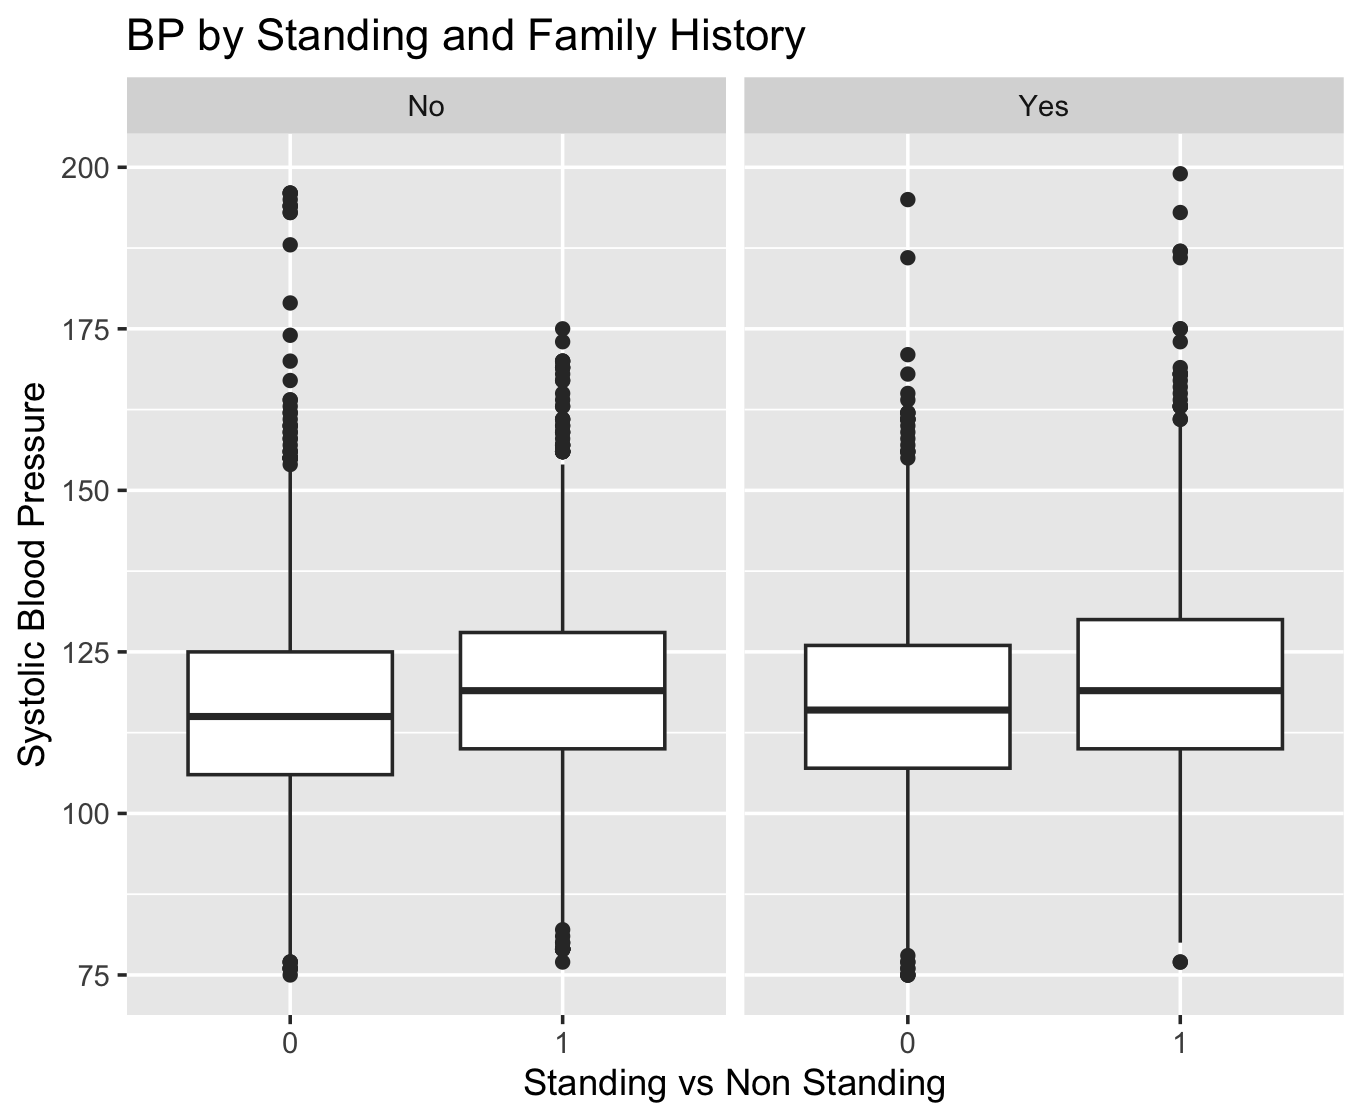
\includegraphics[width=\textwidth]{pics/bp v stand and fh.png}
        \caption{{\small L1 BP vs. Standing by Family History}}
        \label{fig: bp v stand and fh}
    \end{subfigure}
    \hfill
    \begin{subfigure}{0.48\textwidth}
        \centering
        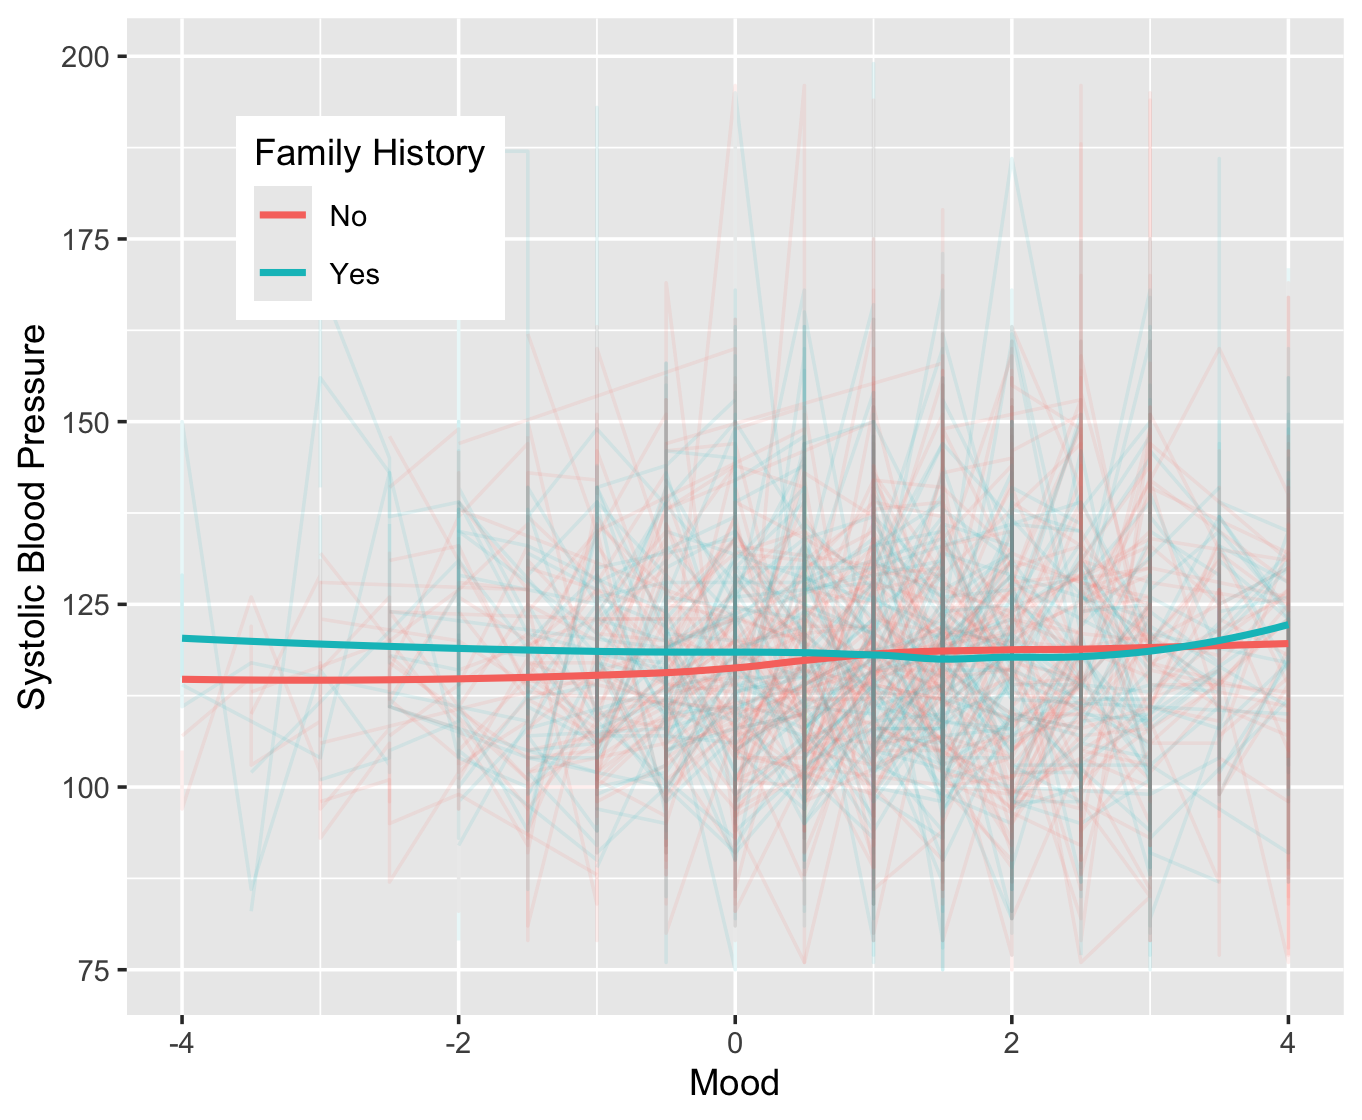
\includegraphics[width=\textwidth]{pics/bp v mood and fh.png}
        \caption{{\small L1 BP vs. Mood by Family History}}
        \label{fig: bp v mood and fh}
    \end{subfigure}
    \caption{{\small L1 BP vs. Level 1 Covariates by Family History}}
    \label{fig: bp v level1 and fh2}
\end{figure}

After fitting separate MLR models for each participant, we see that the intercepts appears to depend on \texttt{Workday} and \texttt{Age} (see \Cref{fig: int v day} and \Cref{fig: int v age}), the slopes for \texttt{Time} appears to depend on \texttt{Family History} and \texttt{Workday} (see \Cref{fig: time v fh} and \Cref{fig: time v day}), and the fixed effect for \texttt{Standing} appears to depend on \texttt{Age} and \texttt{Workday} (see \Cref{fig: stand v age} and \Cref{fig: stand v day}).

\begin{figure} 
    \centering
    \begin{subfigure}[b]{0.32\textwidth}
    \centering
    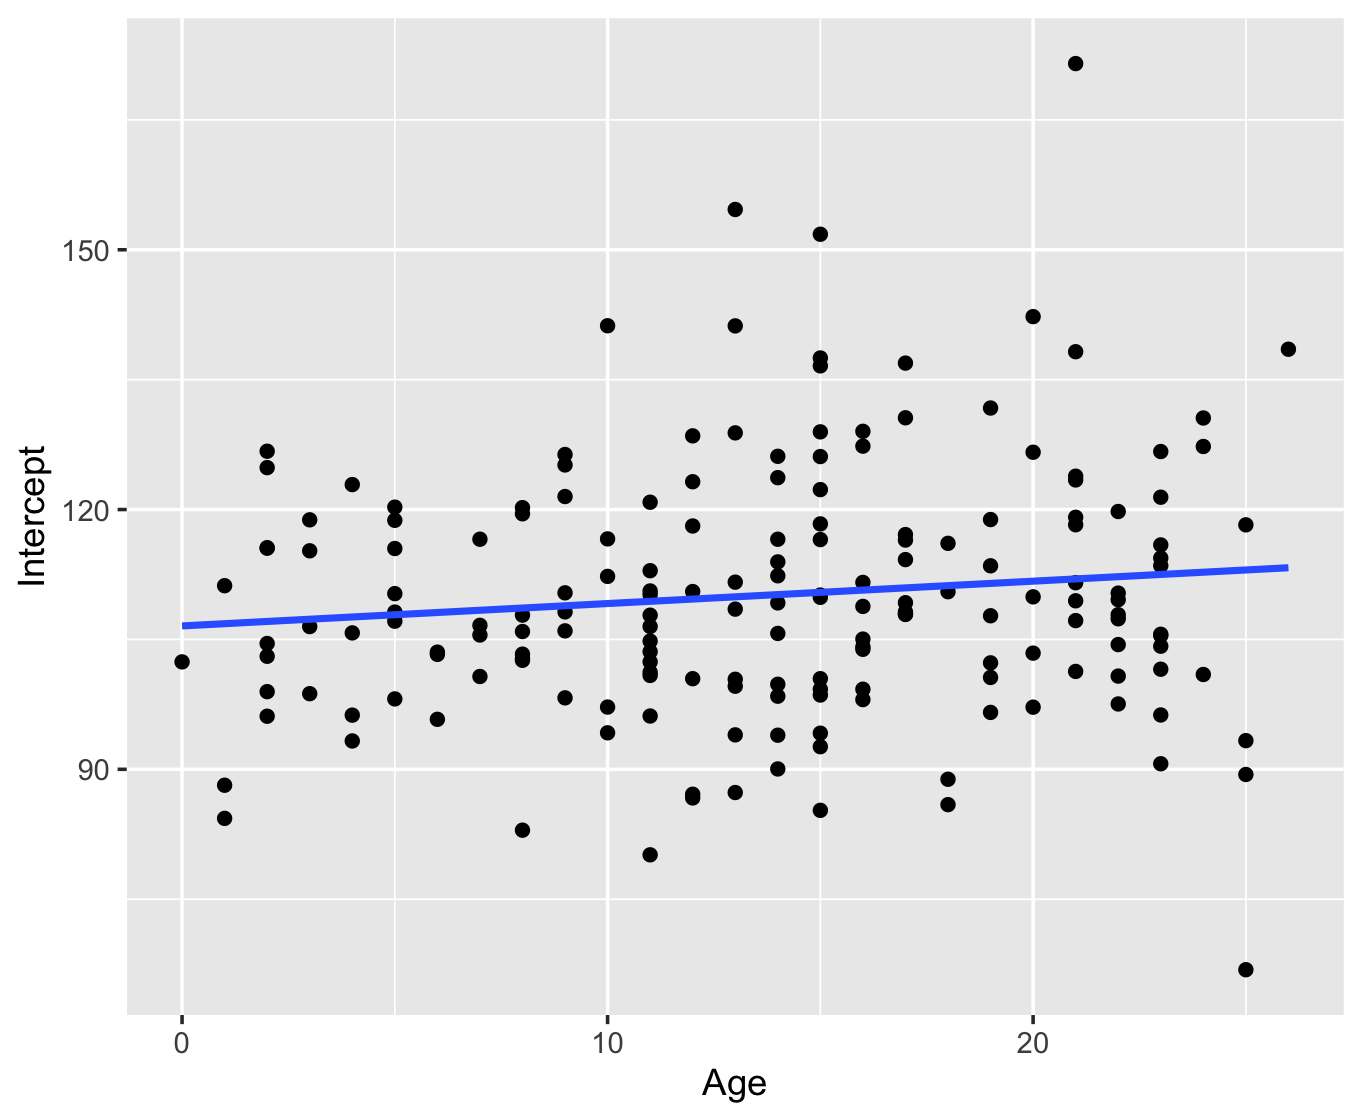
\includegraphics[width=\textwidth]{pics/mlr int by age.png}
    \caption[]%
    {{\small MLR Intercepts by Age}}
    \label{fig: int v age}
    \end{subfigure}
    \hfill
    \begin{subfigure}[b]{0.32\textwidth}
    \centering
    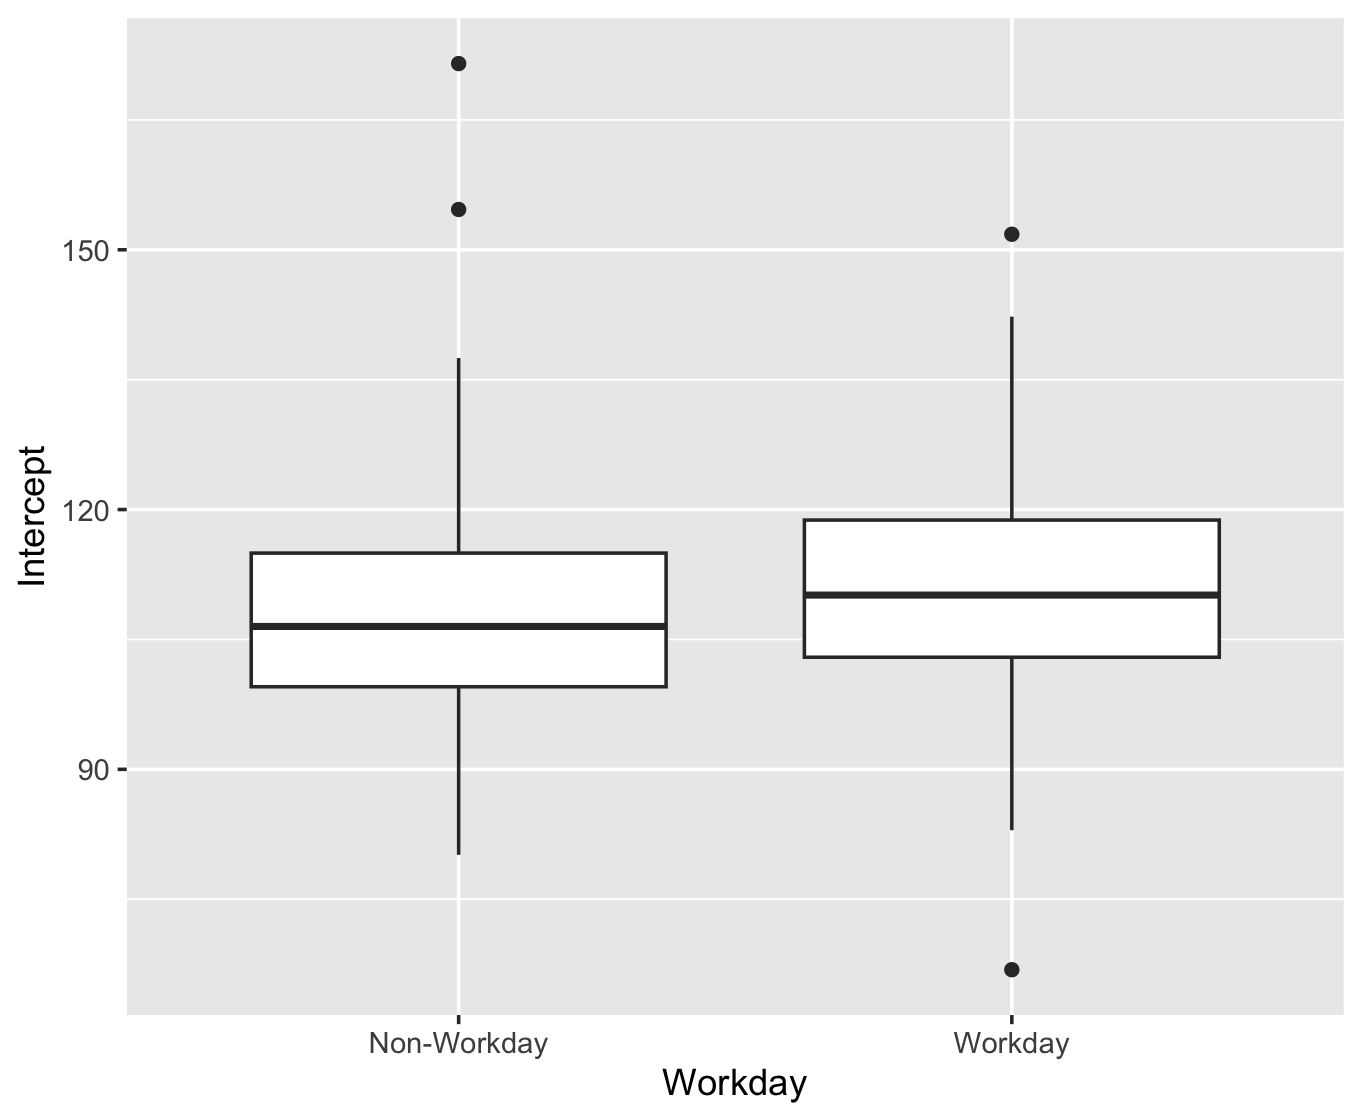
\includegraphics[width=\textwidth]{pics/mlr int by day.png}
    \caption[]%
    {{\small MLR Intercepts by Workday}}
    \label{fig: int v day}
    \end{subfigure}
    \hfill
    \begin{subfigure}[b]{0.32\textwidth}
    \centering
    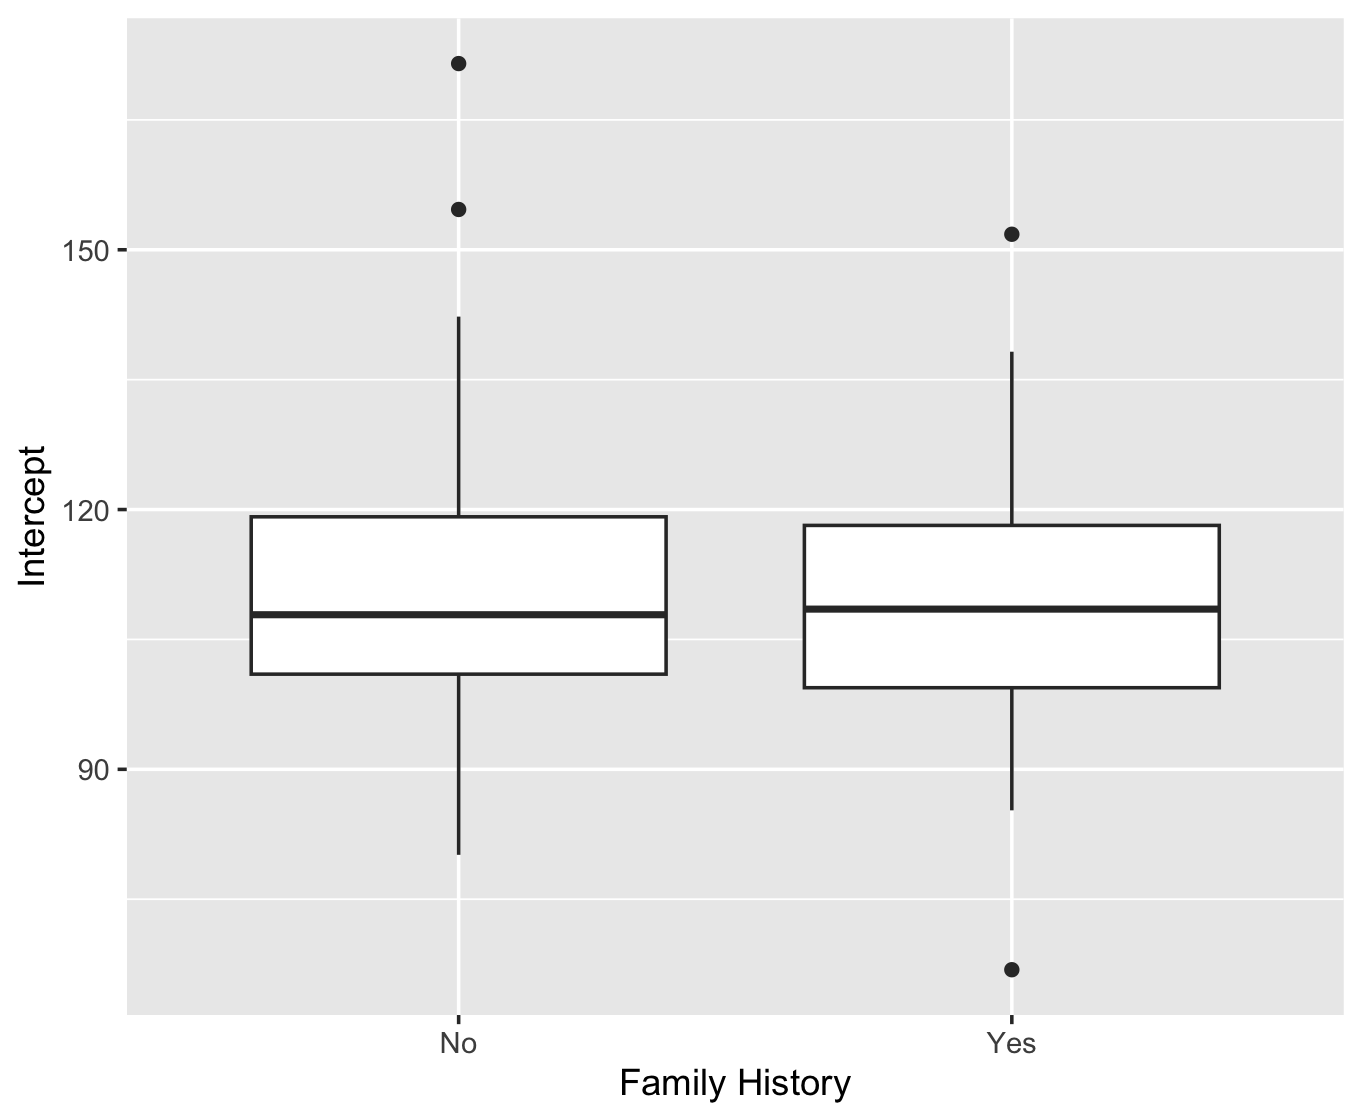
\includegraphics[width=\textwidth]{pics/mlr int by fh.png}
    \caption[]%
    {{\small Intercepts by Family History}}
    \label{fig: int v fh}
    \end{subfigure}
    \caption[]
    {\small MLR Intercepts by Level 2 Covariates}
    \label{fig: int v lv2}
    \end{figure}

    \begin{figure} 
        \centering
        \begin{subfigure}[b]{0.32\textwidth}
        \centering
        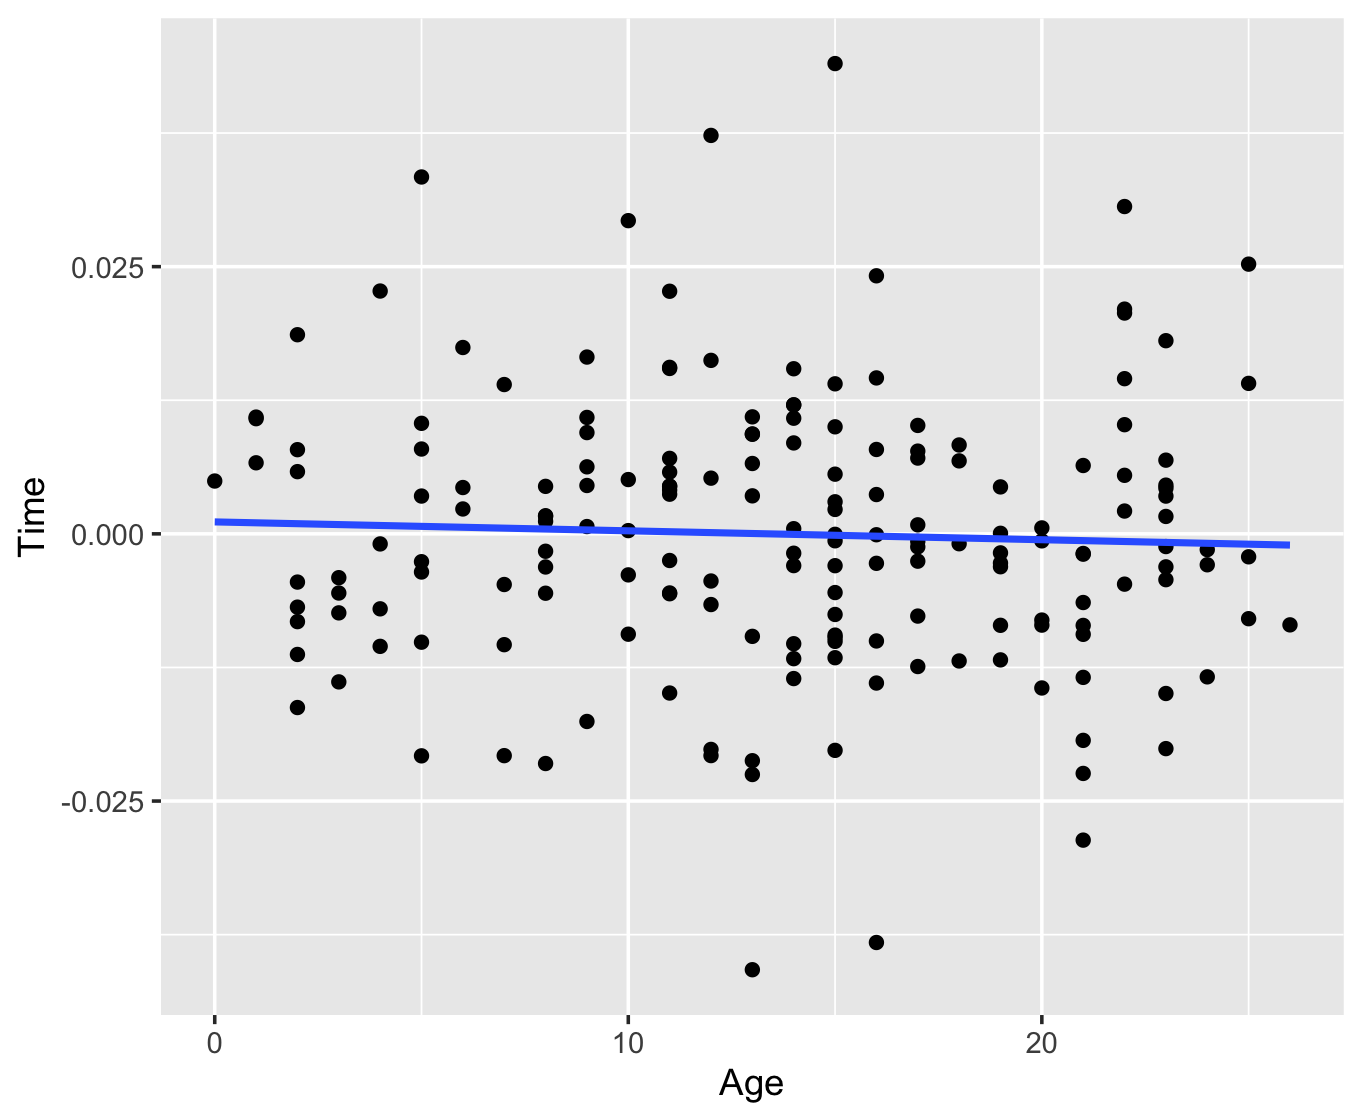
\includegraphics[width=\textwidth]{pics/mlr time by age.png}
        \caption[]%
        {{\small MLR Time by Age}}
        \label{fig: time v age}
        \end{subfigure}
        \hfill
        \begin{subfigure}[b]{0.32\textwidth}
        \centering
        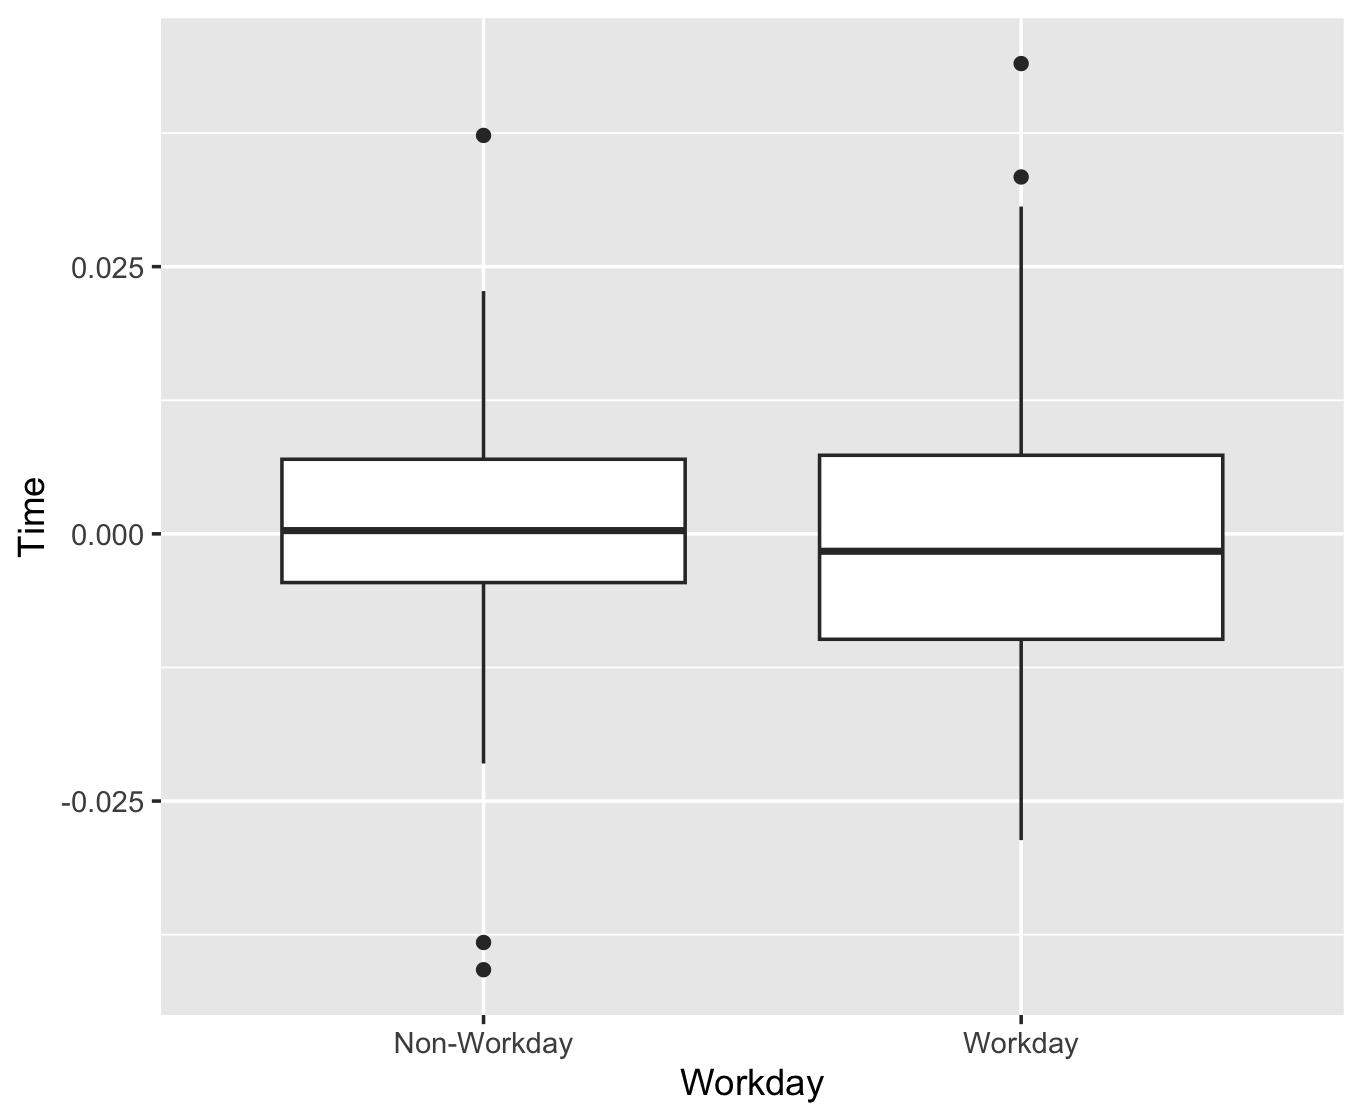
\includegraphics[width=\textwidth]{pics/mlr time by day.png}
        \caption[]%
        {{\small MLR Time by Workday}}
        \label{fig: time v day}
        \end{subfigure}
        \hfill
        \begin{subfigure}[b]{0.32\textwidth}
        \centering
        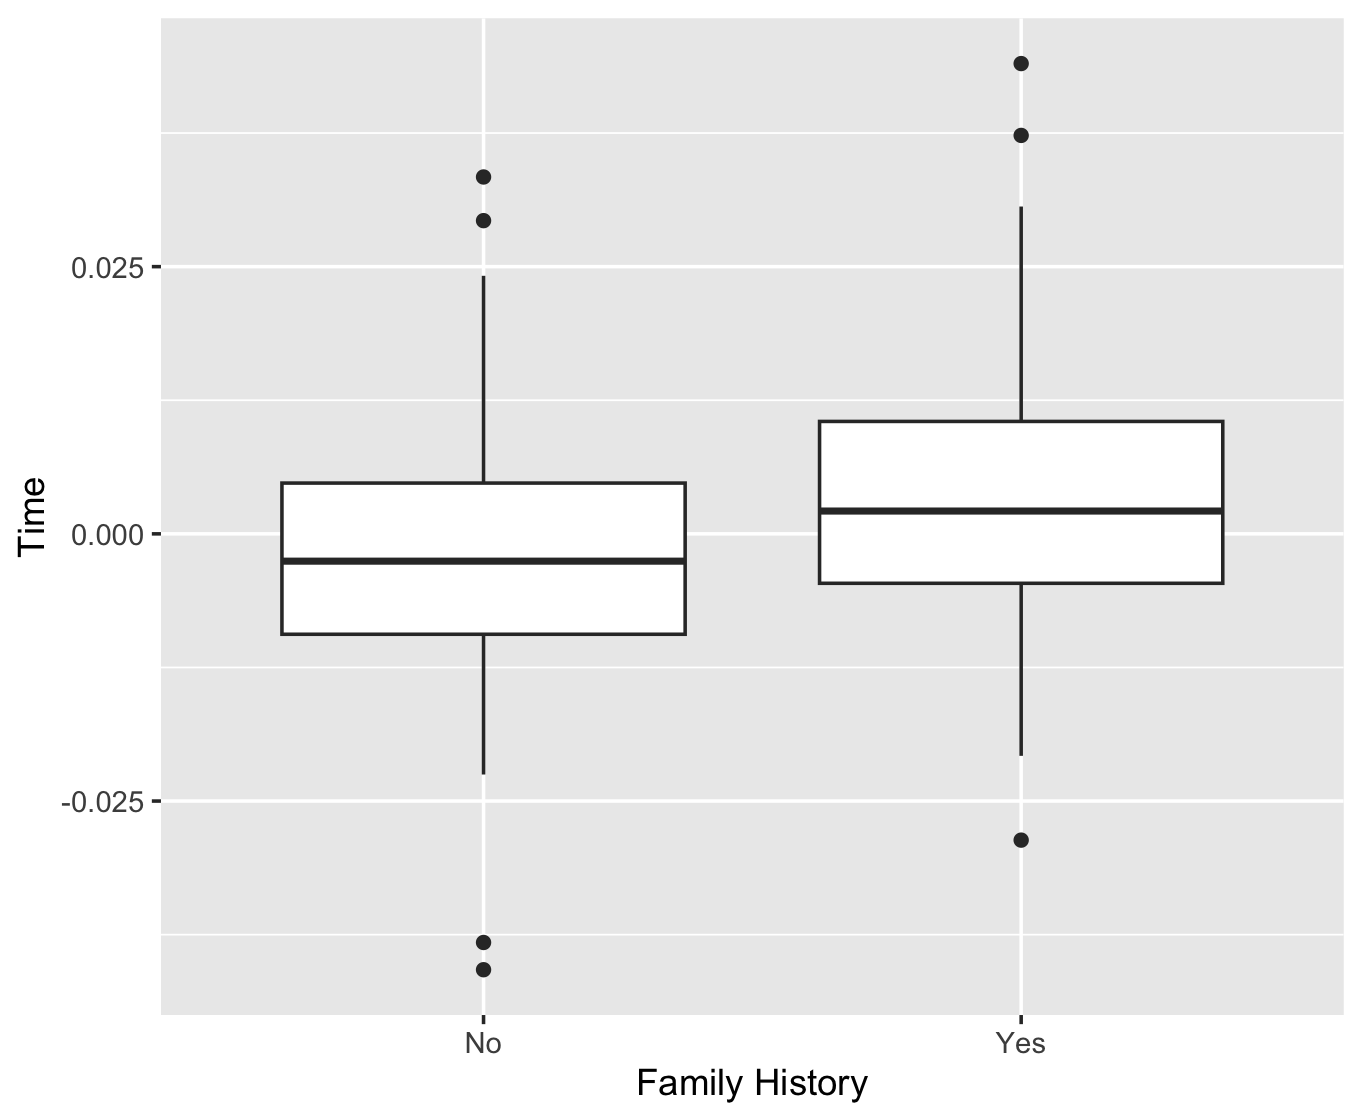
\includegraphics[width=\textwidth]{pics/mlr time by fh.png}
        \caption[]%
        {{\small Time by Family History}}
        \label{fig: time v fh}
        \end{subfigure}
        \caption[]
        {\small MLR Time Slopes by Level 2 Covariates}
        \label{fig: time v lv2}
        \end{figure}
    
        \begin{figure} 
            \centering
            \begin{subfigure}[b]{0.32\textwidth}
            \centering
            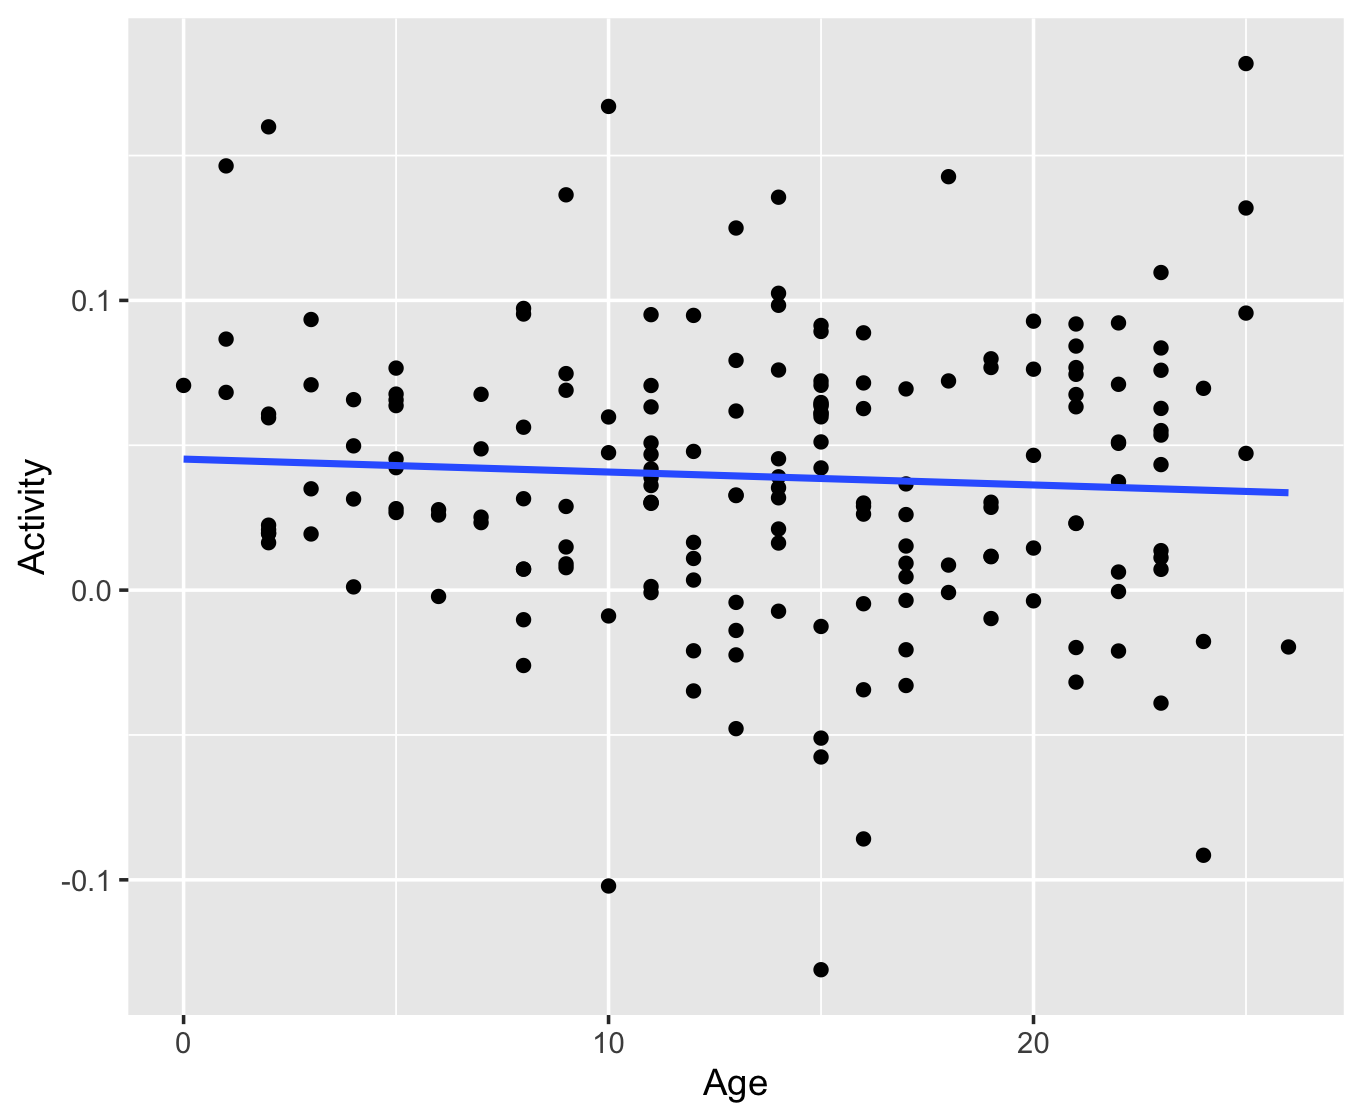
\includegraphics[width=\textwidth]{pics/mlr act by age.png}
            \caption[]%
            {{\small MLR Activity by Age}}
            \label{fig: act v age}
            \end{subfigure}
            \hfill
            \begin{subfigure}[b]{0.32\textwidth}
            \centering
            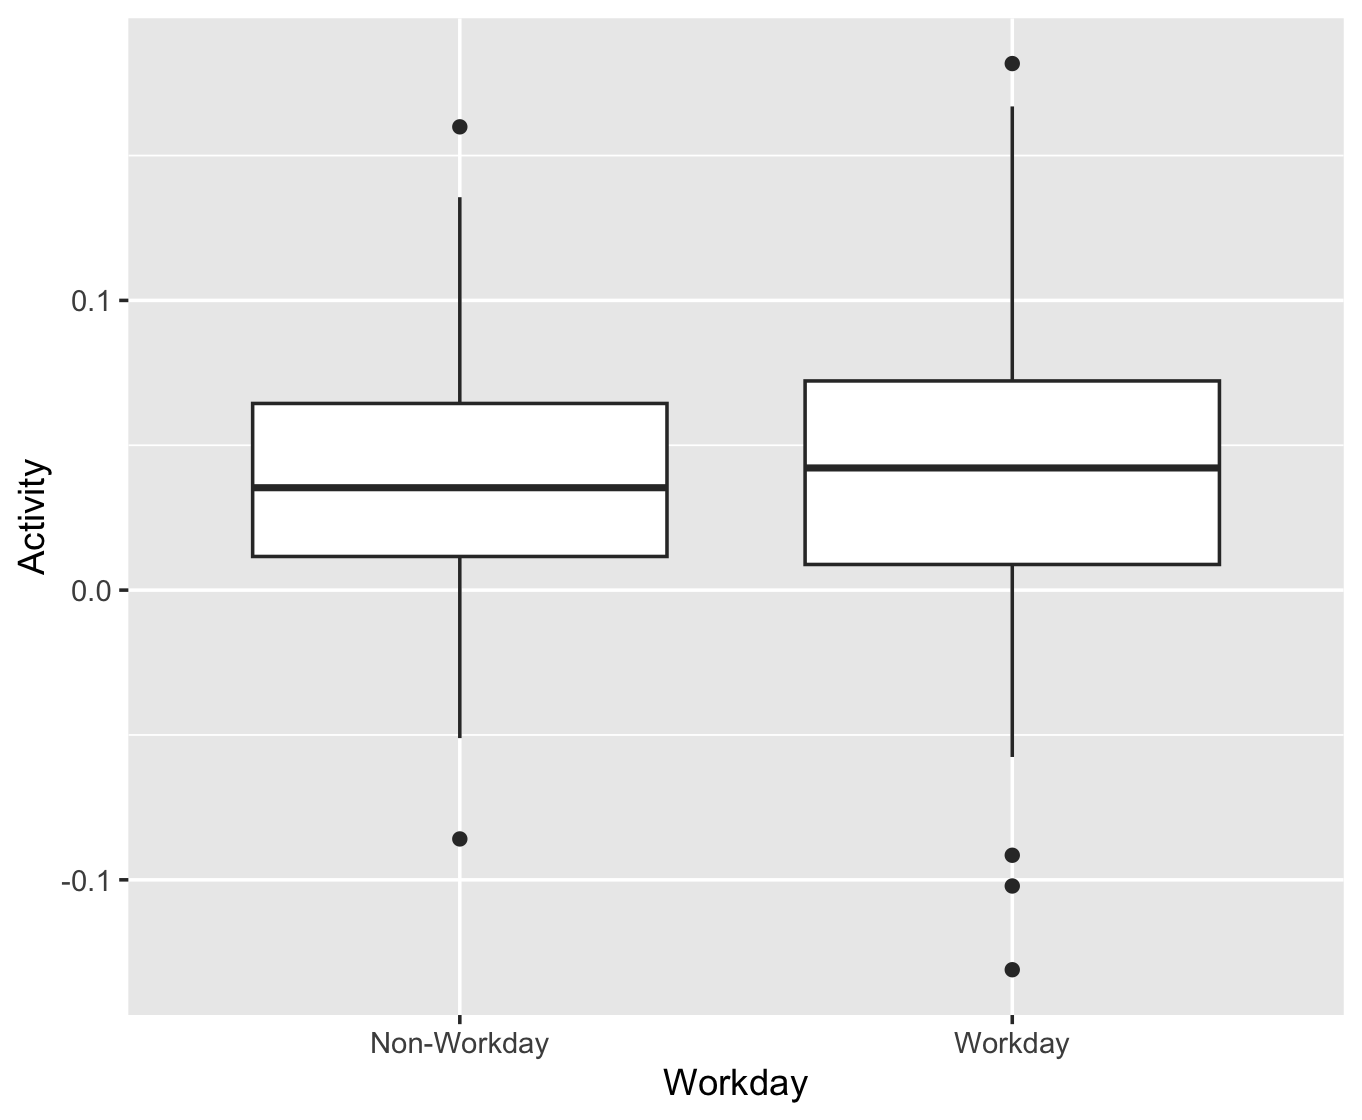
\includegraphics[width=\textwidth]{pics/mlr act by day.png}
            \caption[]%
            {{\small MLR Activity by Workday}}
            \label{fig: act v day}
            \end{subfigure}
            \hfill
            \begin{subfigure}[b]{0.32\textwidth}
            \centering
            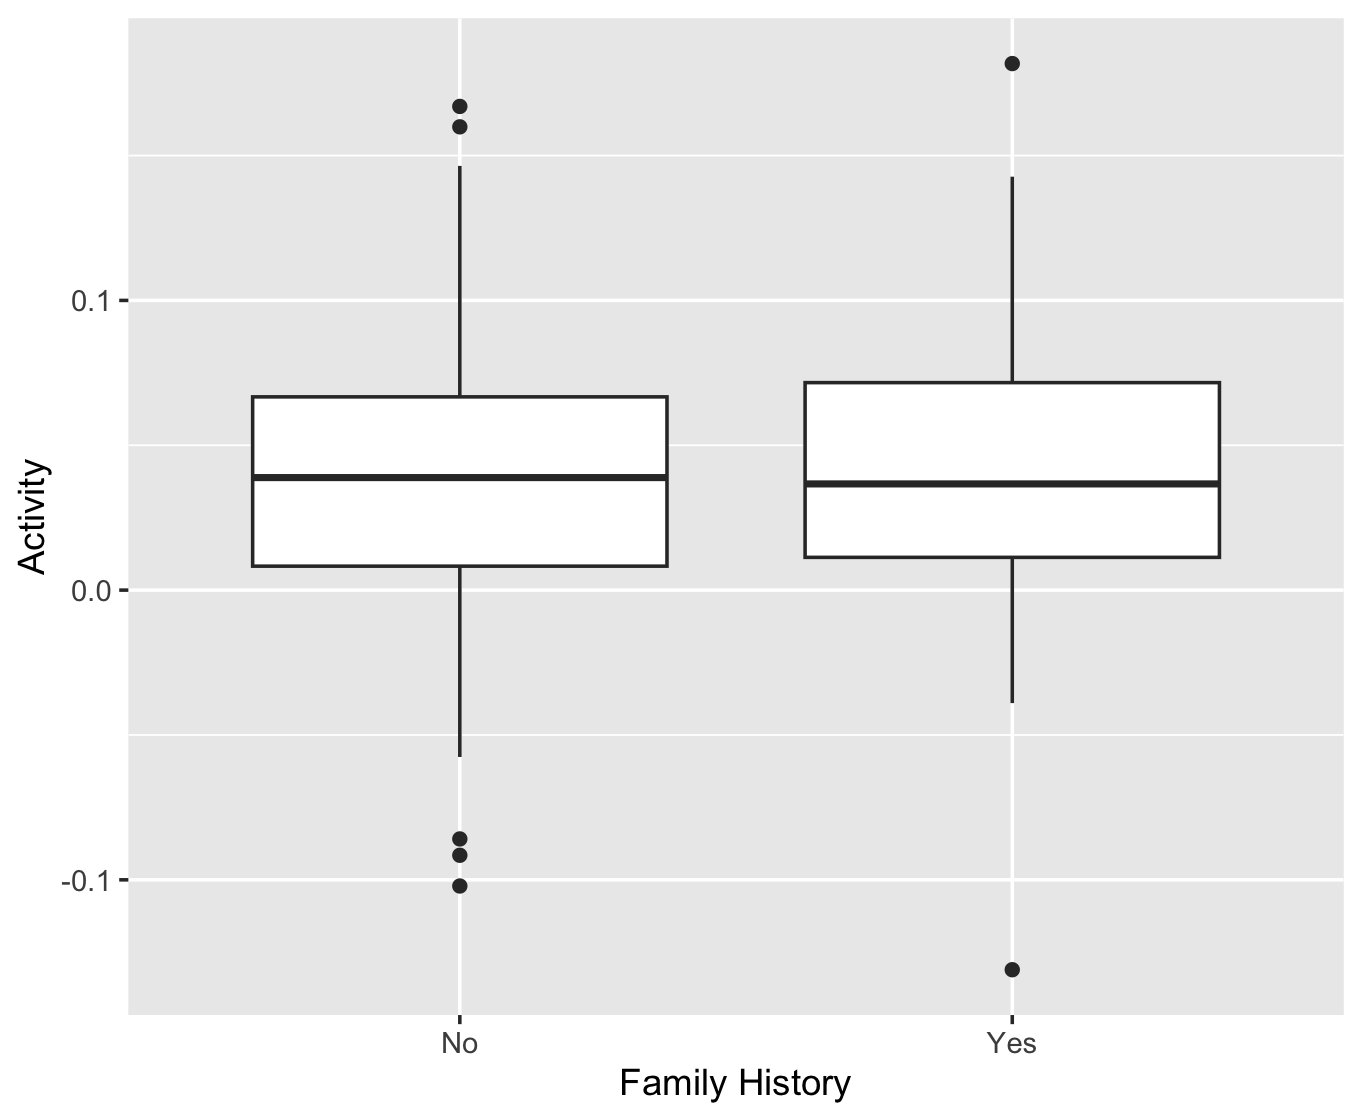
\includegraphics[width=\textwidth]{pics/mlr act by fh.png}
            \caption[]%
            {{\small Activity by Family History}}
            \label{fig: act v fh}
            \end{subfigure}
            \caption[]
            {\small MLR Activity Slopes by Level 2 Covariates}
            \label{fig: act v lv2}
            \end{figure}

            \begin{figure} 
                \centering
                \begin{subfigure}[b]{0.32\textwidth}
                \centering
                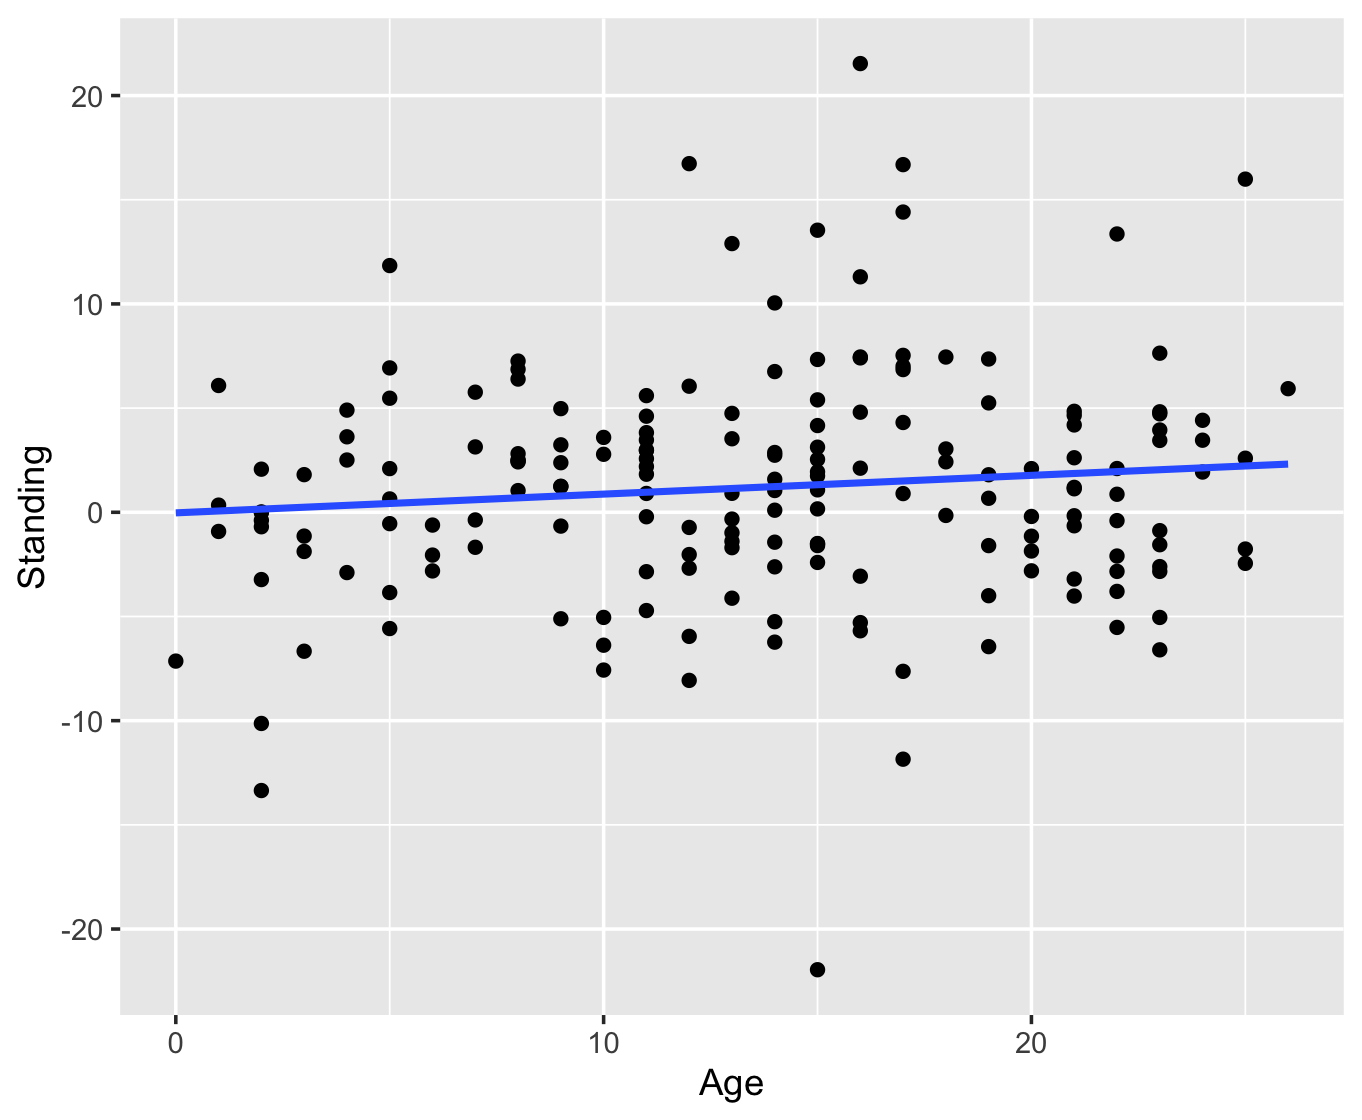
\includegraphics[width=\textwidth]{pics/mlr stand by age.png}
                \caption[]%
                {{\small MLR Standing by Age}}
                \label{fig: stand v age}
                \end{subfigure}
                \hfill
                \begin{subfigure}[b]{0.32\textwidth}
                \centering
                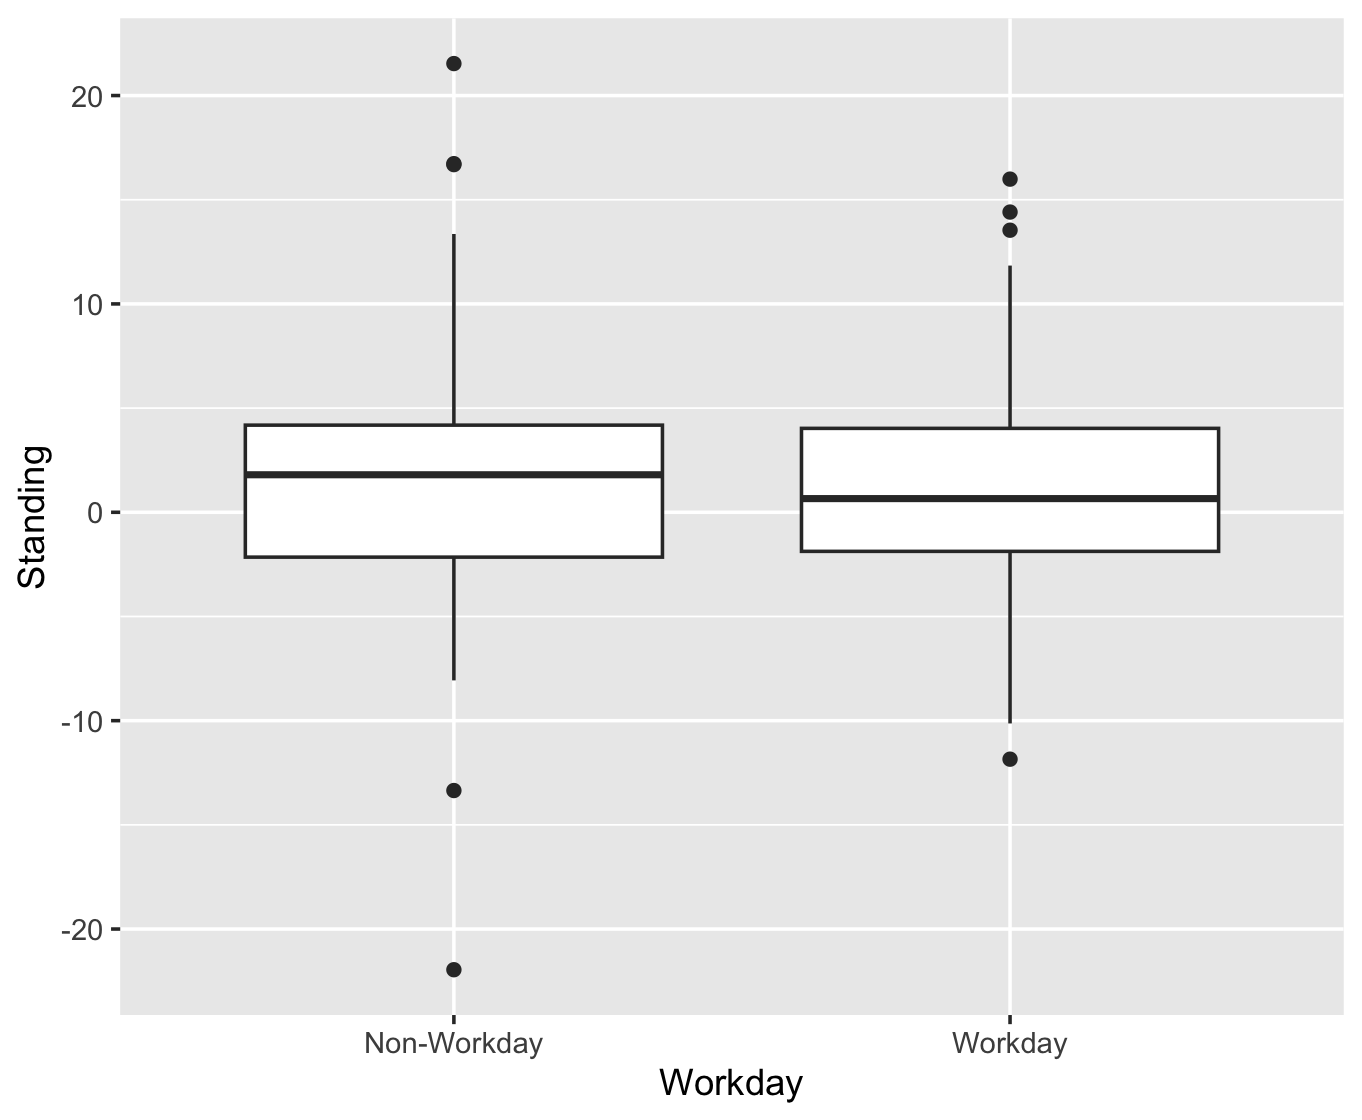
\includegraphics[width=\textwidth]{pics/mlr stand by day.png}
                \caption[]%
                {{\small MLR Standing by Workday}}
                \label{fig: stand v day}
                \end{subfigure}
                \hfill
                \begin{subfigure}[b]{0.32\textwidth}
                \centering
                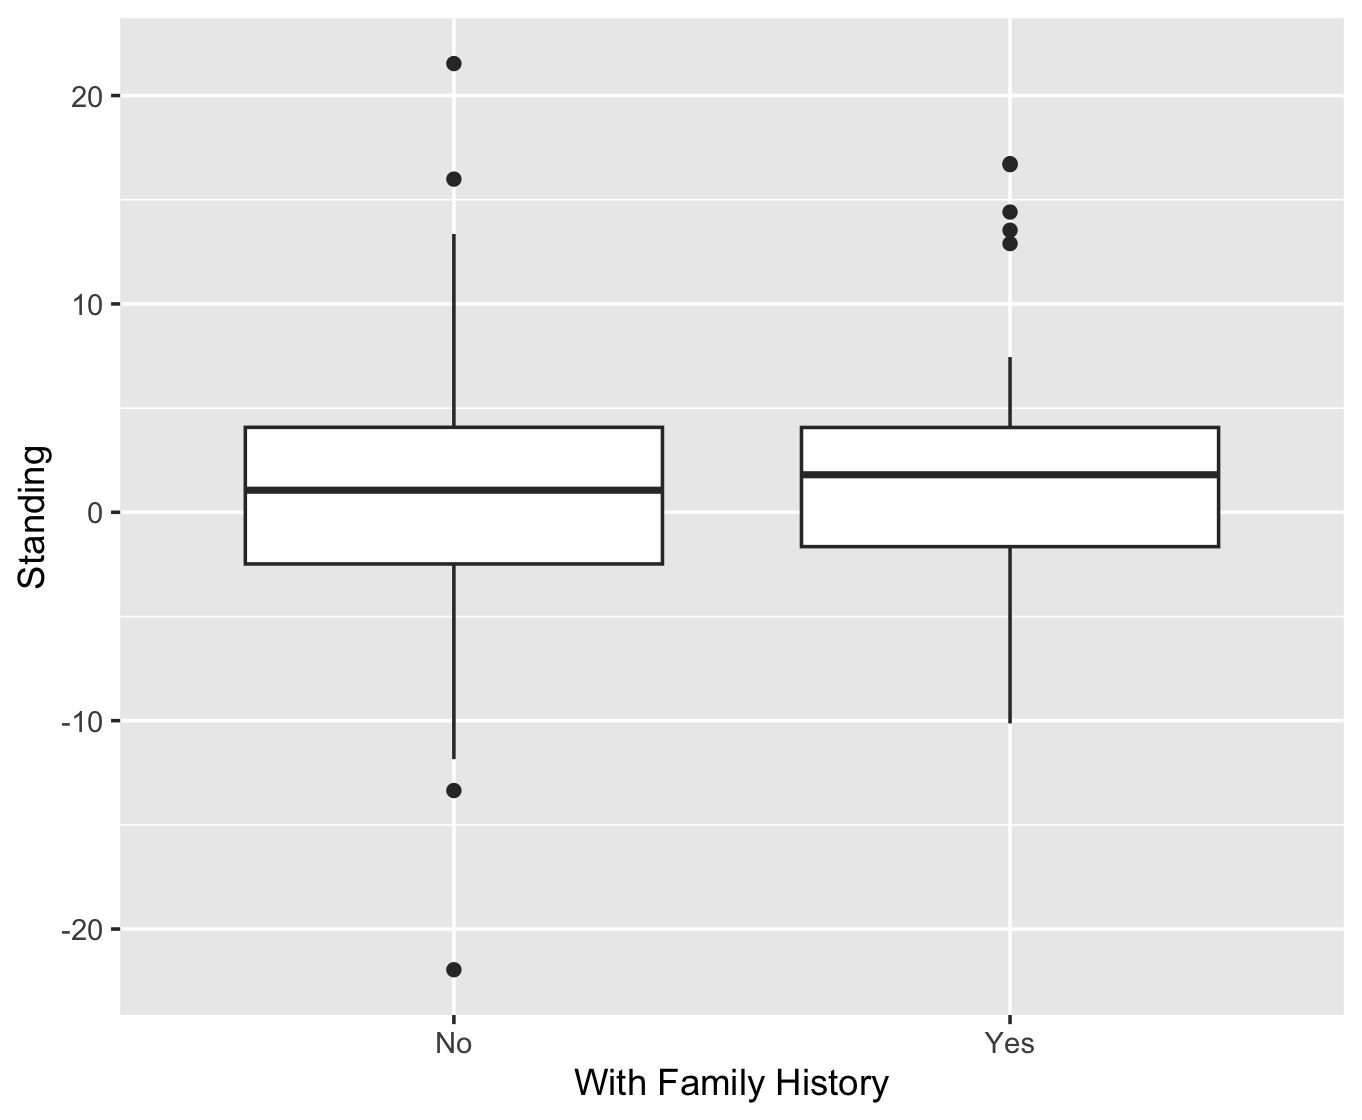
\includegraphics[width=\textwidth]{pics/mlr stand by fh.png}
                \caption[]%
                {{\small Standing by Family History}}
                \label{fig: int v fh}
                \end{subfigure}
                \caption[]
                {\small MLR Standing Fixed Effects by Level 2 Covariates}
                \label{fig: stand v lv2}
                \end{figure}
            
                \begin{figure} 
                    \centering
                    \begin{subfigure}[b]{0.32\textwidth}
                    \centering
                    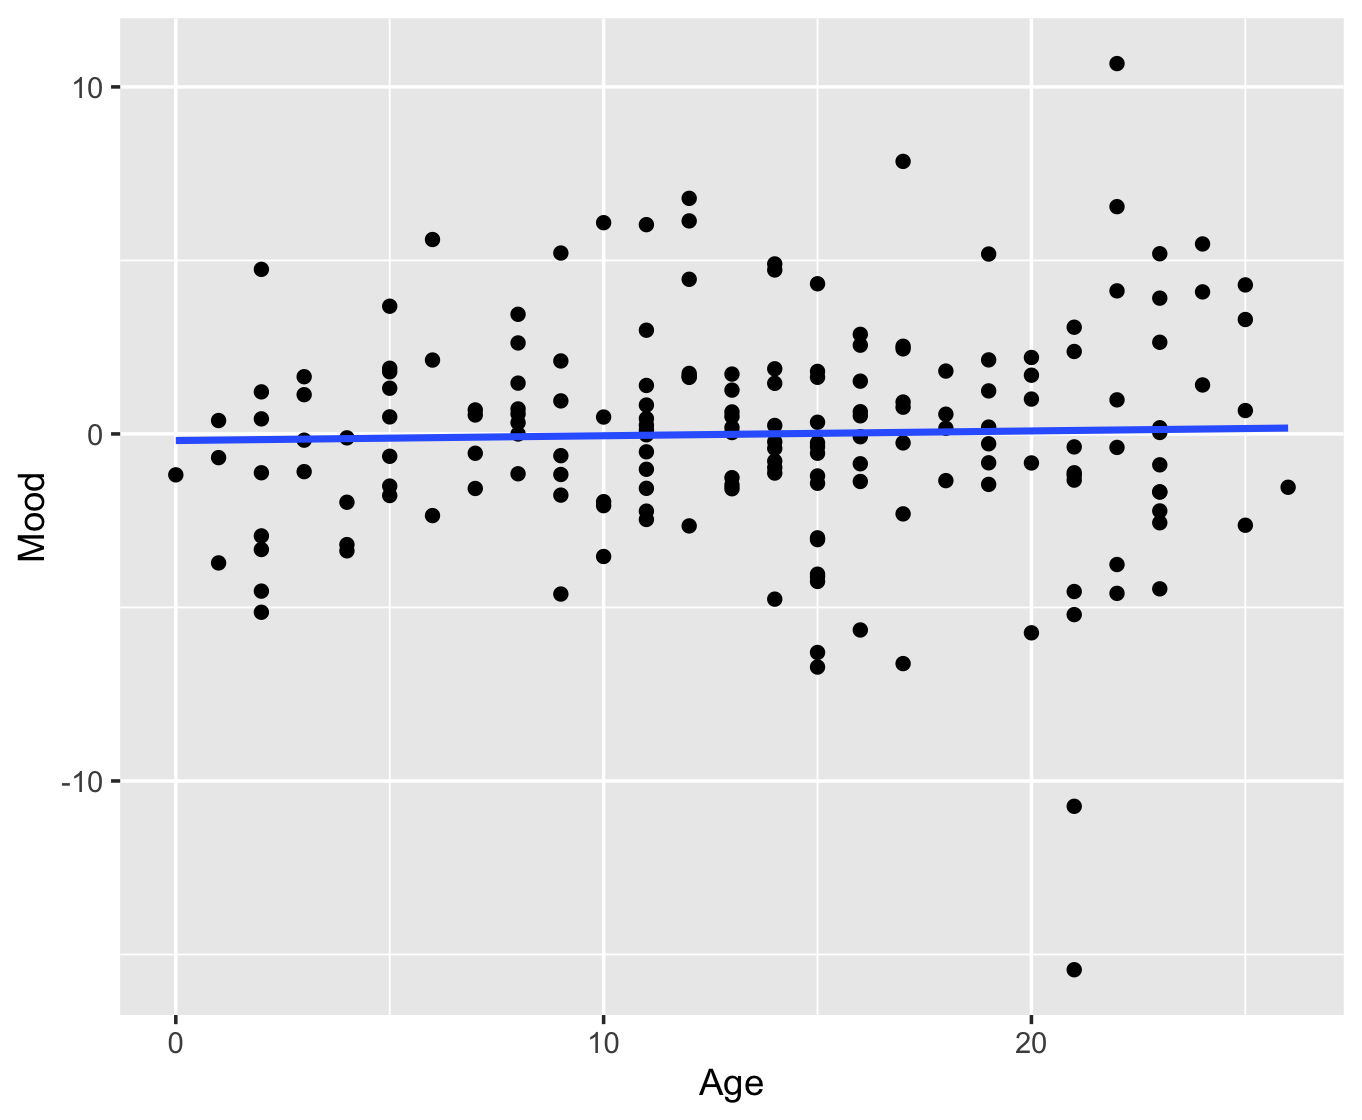
\includegraphics[width=\textwidth]{pics/mlr mood by age.png}
                    \caption[]%
                    {{\small MLR Mood by Age}}
                    \label{fig: mood v age}
                    \end{subfigure}
                    \hfill
                    \begin{subfigure}[b]{0.32\textwidth}
                    \centering
                    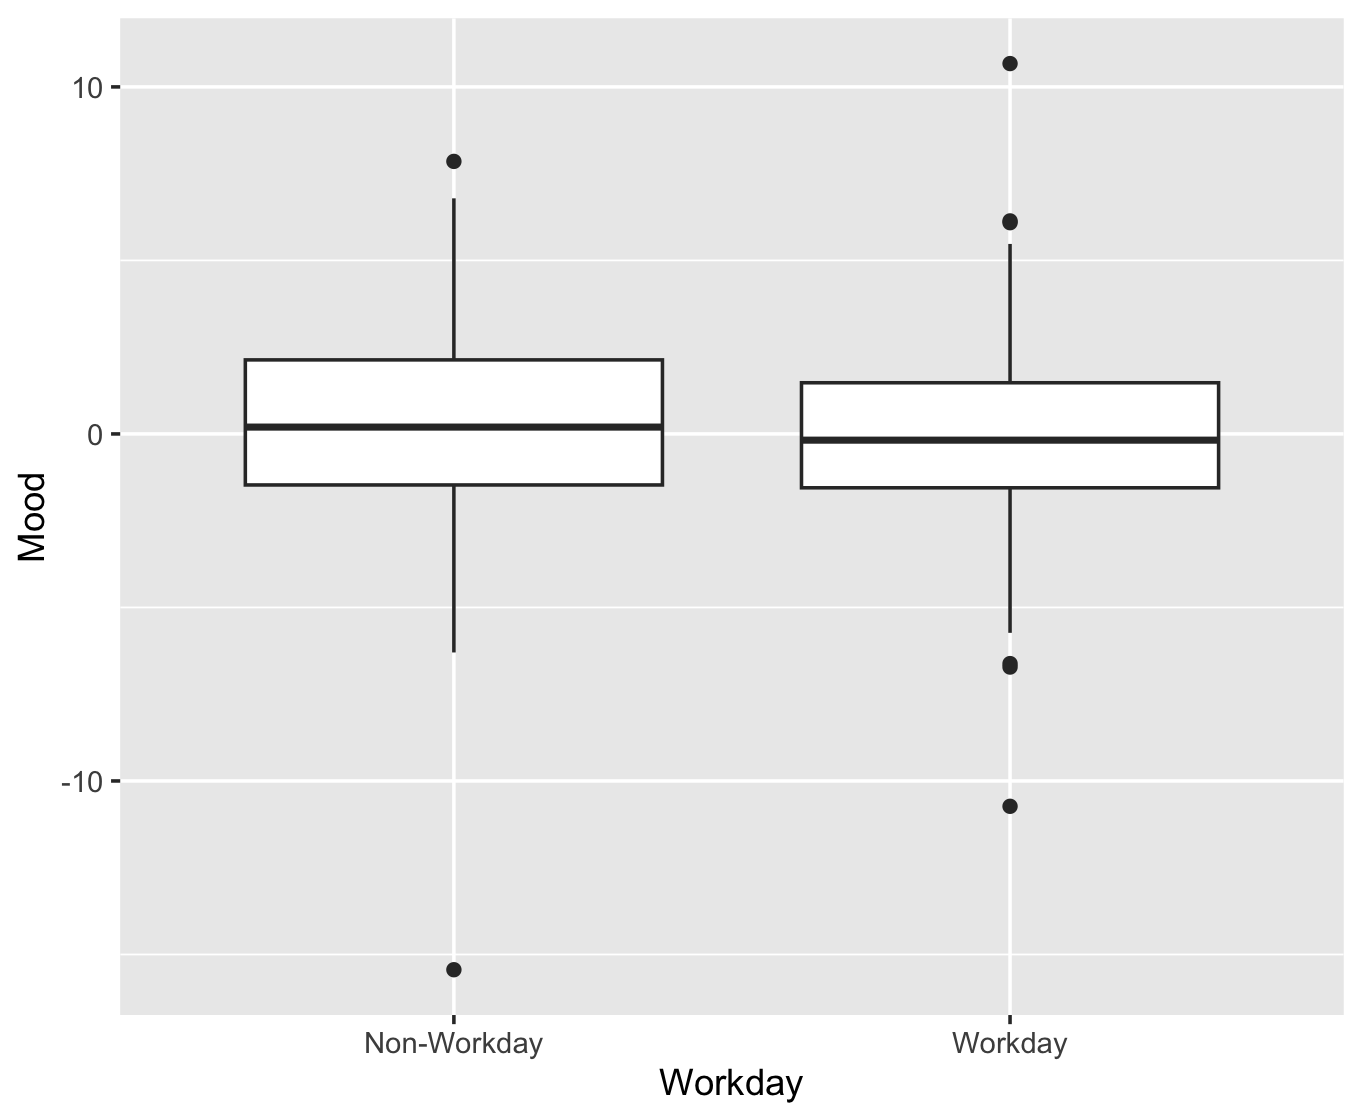
\includegraphics[width=\textwidth]{pics/mlr mood by day.png}
                    \caption[]%
                    {{\small MLR Mood by Workday}}
                    \label{fig: mood v day}
                    \end{subfigure}
                    \hfill
                    \begin{subfigure}[b]{0.32\textwidth}
                    \centering
                    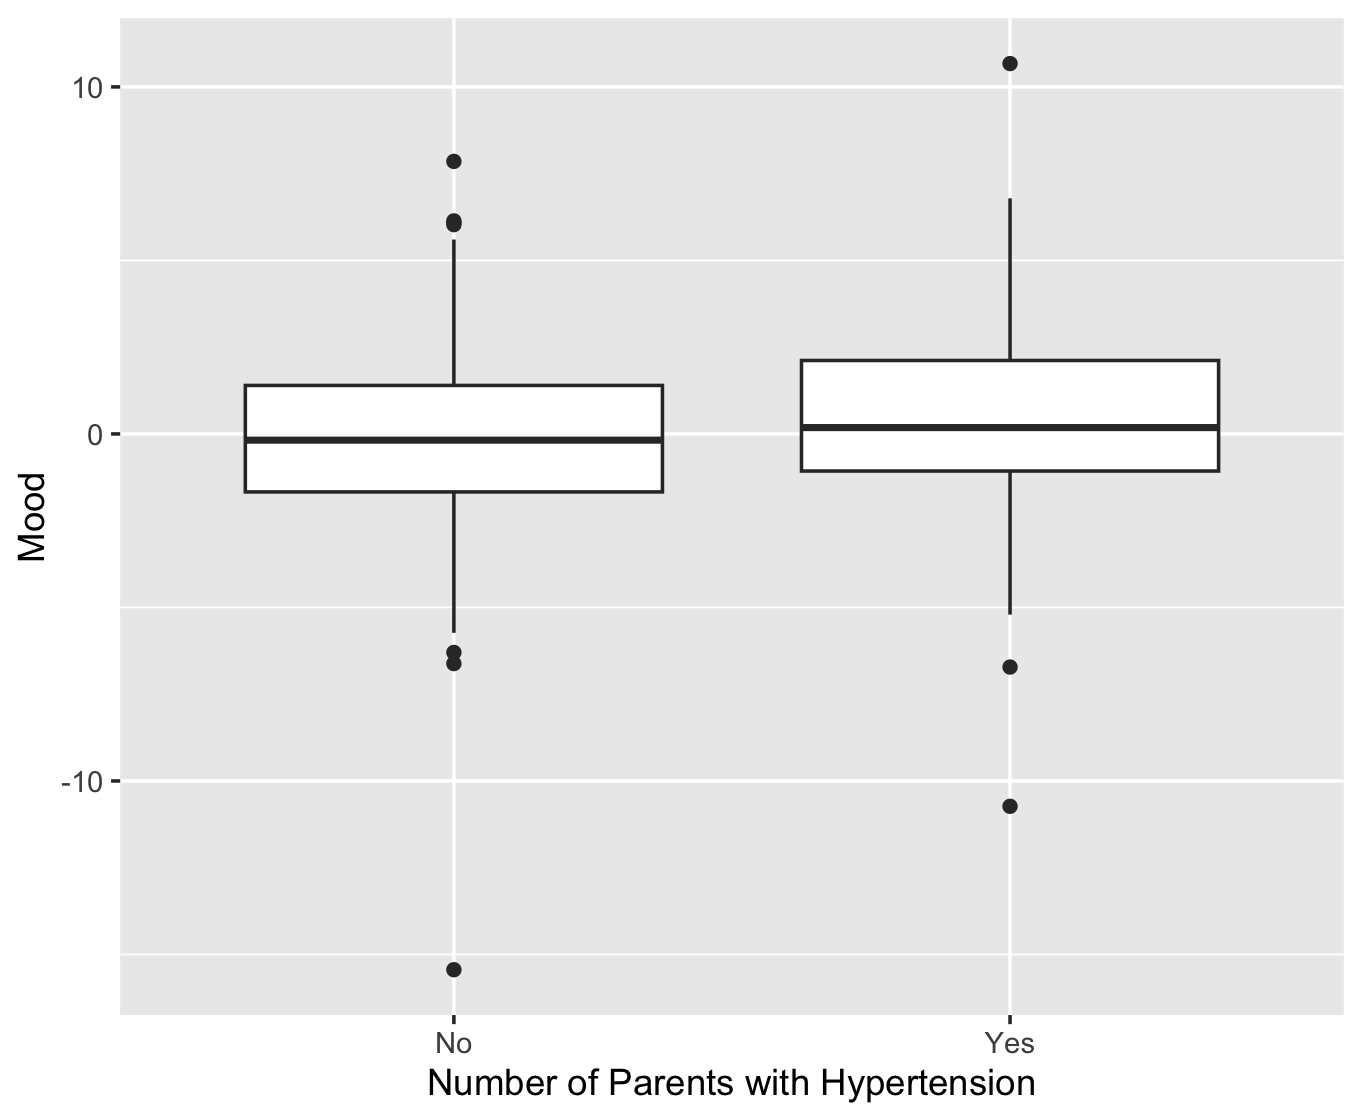
\includegraphics[width=\textwidth]{pics/mlr mood by fh.png}
                    \caption[]%
                    {{\small Mood by Family History}}
                    \label{fig: mood v fh}
                    \end{subfigure}
                    \caption[]
                    {\small MLR Mood Slopes by Level 2 Covariates}
                    \label{fig: mood v lv2}
                    \end{figure}
                

\section{Model Selection}\label{sec: model selection}

We will use a bottom-up approach to build a saturated model from scratch. Since, our data is ordered by time, we start with a base model (Model \ref{eq: RI with time}) with only the random intercept and level 1 covariate time: for the $j^\text{th}$ measurement in the $i^\text{th}$ participant, where $i = 1,\, \ldots,\, n$ and $j = 1,\, \ldots,\, n_i$,
\begin{equation}\label{eq: RI with time}
    \begin{aligned}
        \text{Level 1}: \quad & \text{BP}_{ij} &&= a_i + \beta_1\, \text{Time}_{ij} + \epsilon_{ij}, \quad & \epsilon_{ij} &\overset{i.i.d.}{\sim} N(0, \sigma^2) \\
        \text{Level 2}: \quad & a_i &&= \alpha + u_i, \quad & u_{i} &\overset{i.i.d.}{\sim} N(0, \sigma_u^2).
    \end{aligned}
\end{equation}
A Likelihood Ration Test (LRT) reveals that compared to a Ordinary Least Squares (OLS) model with no random intercept, the random effect is significant ($\chi^2 (0,\, 1) = 2044.1$, $p < 2.2 \times 10^{-16}$). Note that here the $p$-value is a mixture from a chi-square model with 0 degrees of freedom and 1 degree of freedom.

We then proceed to add in fixed effects for level 1 to investigate whether activity level, whether or not the participants were standing, and mood ratings were \emph{associated} with elevating BP. We propose the following (Model \ref{eq: RI with all lv1}) with a random intercept and all level 1 covariates:
\begin{equation}\label{eq: RI with all lv1}
    \begin{array}{rrcll}
        \text{Level 1}: & \text{BP}_{ij} &=& a_i + \beta_1\, \text{Time}_{ij} + \beta_2\, \text{Activity}_{ij} + \beta_3\, \text{Standing}_{ij} + \\
        &&& \beta_4\, \text{Mood}_{ij} + \epsilon_{ij}, \\[0.5ex]
         & \epsilon_{ij} &\overset{i.i.d.}{\sim}& N(0, \sigma^2), \\[0.5ex]
        \text{Level 2}: & a_i &=& \alpha + u_i, \\[0.5ex]
         & u_{i} &\overset{i.i.d.}{\sim}& N(0, \sigma_u^2).
    \end{array}
\end{equation}
A LRT between Model \ref{eq: RI with time} and \ref{eq: RI with all lv1} reveals that the three added fixed effects are statistically significant ($\chi^2 (3) = 365.37$, $p < 2.2 \times 10^{-16}$). Naturally, one might wonder if we need all three fixed effect. Indeed, a LRT suggests that the following Model \ref{eq: RI no mood} without the covariate \texttt{Mood} ($\beta_4 = 0$) is just as good as Model \ref{eq: RI with all lv1} ($\chi^2 (1) = 0.43$, $p =0.51$). Because we are interested in \emph{whether} something is associated with elevated \texttt{BP} at all, we proceed the analysis with the simpler Model \ref{eq: RI no mood}.
\begin{equation}\label{eq: RI no mood}
    \begin{array}{rrcll}\tag{\ref{eq: RI with all lv1}$'$}
        \text{Level 1}: & \text{BP}_{ij} &=& a_i' + \beta_1'\, \text{Time}_{ij} + \beta_2'\, \text{Activity}_{ij} + \beta_3'\, \text{Standing}_{ij} + \epsilon_{ij}, \\[0.5ex]
         & \epsilon_{ij} &\overset{i.i.d.}{\sim}& N(0, \sigma^2), \\[0.5ex]
        \text{Level 2}: & a_i' &=& \alpha' + u_i, \\[0.5ex]
         & u_{i} &\overset{i.i.d.}{\sim}& N(0, \sigma_u^2).
    \end{array}
\end{equation}
Interestingly, LRT tests also suggest that compared to Model \ref{eq: RI no mood}, a model without the \texttt{Time} term ($\beta_1' = 0$) is also just as good ($\chi^2 (1) = 0.99$, $p = 0.32$). However, because time is such an important aspect of the longitudinal model, we think it is important that we keep \texttt{Time} as a level 1 covariate in our model.

Next we investigate what random effects are needed in our model. The most clear evidence of random slopes from our EDA comes from \texttt{Mood}, but since LRT tests suggest that the fixed effect of \texttt{Mood} is not significant, we will not consider its random effect. For the rest of the covariates, EDA do show marginal signs of varying slopes. However, only adding a random effect for \texttt{Standing} do not raise convergence issues. This leads us to the following model with a random effect for \texttt{Standing}:
\begin{equation}\label{eq: RIS stand}
    \begin{array}{rrcll}
        \text{Level 1}: & \text{BP}_{ij} &=& a_i + \gamma_1\, \text{Time}_{ij} + \gamma_2\, \text{Activity}_{ij} + b_i\, \text{Standing}_{ij} + \epsilon_{ij}, \\[0.5ex]
         & \epsilon_{ij} &\overset{i.i.d.}{\sim}& N(0, \sigma^2), \\[0.5ex]
        \text{Level 2}: & a_i &=& \alpha + u_i, \\[0.5ex]
         & b_i &=& \beta + v_i, \\[1ex]
         & \begin{bmatrix} u_i \\ v_i 
         \end{bmatrix} &\overset{i.i.d.}{\sim}& N_2\left(\begin{bmatrix} 0 \\ 0 \end{bmatrix},\, \begin{bmatrix} \sigma_u^2 &\\ 
         \rho_{uv}\sigma_u\sigma_v & \sigma_v^2\\
         \end{bmatrix} \right).
    \end{array}
\end{equation}
A LRT suggests that the random effect for \texttt{Standing} is significant, based on a mixture from a chi-square model with 1 and 2 degrees of freedom ($\chi^2 (1,\, 2) = 377.34.1$, $p < 2.2 \times 10^{-16}$). Interestingly, removing the correlation term ($\rho_{uv}$) between the random effect for the intercept and the random effect for \texttt{Standing} causes further convergence issues, so we preserve the it in our following analysis.

We move on to consider the interaction between level 2 and level 1 covaraites. Recall that our EDA identifies \texttt{Age}, \texttt{Workday}, and \texttt{Family History} as possibly interacting with the effect for \texttt{Standing}, the effects for \texttt{Time} and \texttt{Standing}, and the effect for \texttt{Time}, respectively. We will first consider whether the intercept and the effect of \texttt{Standing} depend on \texttt{Age} (recentered at 24):
\begin{equation}\label{eq: RIS stand age}
    \begin{array}{rrcll}
        \text{Level 1}: & \text{BP}_{ij} &=& a_i + \gamma_1\, \text{Time}_{ij} + \gamma_2\, \text{Activity}_{ij} + b_i\, \text{Standing}_{ij} + \epsilon_{ij}, \\[0.5ex]
         & \epsilon_{ij} &\overset{i.i.d.}{\sim}& N(0, \sigma^2), \\[0.5ex]
        \text{Level 2}: & a_i &=& \alpha + \alpha_1\, \text{Age}_i + u_i, \\[0.5ex]
         & b_i &=& \beta + \beta_1\, \text{Age}_i + v_i, \\[1ex]
         & \begin{bmatrix} u_i \\ v_i 
         \end{bmatrix} &\overset{i.i.d.}{\sim}& N_2\left(\begin{bmatrix} 0 \\ 0 \end{bmatrix},\, \begin{bmatrix} \sigma_u^2 &\\ 
         \rho_{uv}\sigma_u\sigma_v & \sigma_v^2\\
         \end{bmatrix} \right).
    \end{array}
\end{equation}
When compared with Model \ref{eq: RIS stand} ($\alpha_1 = \beta_1 = 0$), a LRT suggests that the smaller model without \texttt{Age} is just as good as the full model with the \texttt{Age} term ($\chi^2 (2) = 0.97$, $p = 0.61$). Because this project concerns \emph{whether} a covaraite is associated with elevated \texttt{BP}, we will proceed with the smaller model without \texttt{Age}.\footnote{Note that \citet{goldstein_ambulatory_2000} does include \texttt{Age} as a predictor because they are interested in preventative measures \emph{controlling for} age. This is not the aim of this project, even though \texttt{Age} is a meaningful and important predictor.} 

Next, we consider the interaction of \texttt{Workday} between \texttt{Time} and \texttt{Standing}. 
\begin{equation}\label{eq: RIS workday}
    \begin{array}{rrcll}
        \text{Level 1}: & \text{BP}_{ij} &=& a_i + b_i\, \text{Time}_{ij} + \delta \, \text{Activity}_{ij} + c_i\, \text{Standing}_{ij} + \epsilon_{ij}, \\[0.5ex]
         & \epsilon_{ij} &\overset{i.i.d.}{\sim}& N(0, \sigma^2), \\[0.5ex]
        \text{Level 2}: & a_i &=& \alpha_0 + \alpha_1\, \text{Workday}_i + u_i, \\[0.5ex]
        & b_i &=& \beta_0 + \beta_1\, \text{Workday}_i \\[0.5ex]
        & c_i &=& \gamma_0 + \gamma_1\, \text{Workday}_i + v_i, \\[1ex]
         & \begin{bmatrix} u_i \\ v_i 
         \end{bmatrix} &\overset{i.i.d.}{\sim}& N_2\left(\begin{bmatrix} 0 \\ 0 \end{bmatrix},\, \begin{bmatrix} \sigma_u^2 &\\ 
         \rho_{uv}\sigma_u\sigma_v & \sigma_v^2\\
         \end{bmatrix} \right).
    \end{array}
\end{equation}
A LRT suggests that, when compared to Model \ref{eq: RIS stand} ($\alpha_1 = \beta_1 = \gamma_1 = 0$), at least one of coefficients is statistically significantly different from zero; we have some evidence to reject the Model \ref{eq: RIS stand} and prefer Model \ref{eq: RIS workday} for better model fit ($\chi^2 (3) = 8.22$, $p = 0.04$). However, when one removes the interaction between \texttt{Workday} and \texttt{Standing} ($\gamma_1 = 0$), a LRT test suggests that the smaller model is just as good ($\chi^2 (1) = 0.45$, $p = 0.50$); we drop the $\gamma_1$ for the sake of simplicity, which, when compared to the simpler Model \ref{eq: RIS stand} ($\alpha_1 = \beta_1 = 0$), still presents better explanatory power ($\chi^2 (2) = 7.77$, $p = 0.02$). Nevertheless, if we were to remove the interaction between \texttt{Time} and \texttt{Workday} ($\beta_1 = \gamma_1 = 0$ vs. $\gamma_1 = 0$), a LRT suggests that we have some evidence to prefer having the interaction between \texttt{Time} and \texttt{Workday} for a better model fit ($\chi^2 (1) = 4.46$, $p = 0.03$):
\begin{equation}\label{eq: RIS workday no stand}
    \begin{array}{rrcll}\tag{\ref{eq: RIS workday}$'$}
        \text{Level 1}: & \text{BP}_{ij} &=& a_i + b_i\, \text{Time}_{ij} + \delta \, \text{Activity}_{ij} + c_i\, \text{Standing}_{ij} + \epsilon_{ij}, \\[0.5ex]
         & \epsilon_{ij} &\overset{i.i.d.}{\sim}& N(0, \sigma^2), \\[0.5ex]
        \text{Level 2}: & a_i &=& \alpha_0 + \alpha_1\, \text{Workday}_i + u_i, \\[0.5ex]
        & b_i &=& \beta_0 + \beta_1\, \text{Workday}_i \\[0.5ex]
        & c_i &=& \gamma_0 + v_i, \\[1ex]
         & \begin{bmatrix} u_i \\ v_i 
         \end{bmatrix} &\overset{i.i.d.}{\sim}& N_2\left(\begin{bmatrix} 0 \\ 0 \end{bmatrix},\, \begin{bmatrix} \sigma_u^2 &\\ 
         \rho_{uv}\sigma_u\sigma_v & \sigma_v^2\\
         \end{bmatrix} \right).
    \end{array}
\end{equation}

Lastly, we will consider the interaction between \texttt{Family History} and \texttt{Time}:
\begin{equation}\label{eq: RIS workday fh}
    \begin{array}{rrcll}
        \text{Level 1}: & \text{BP}_{ij} &=& a_i + b_i\, \text{Time}_{ij} + \delta \, \text{Activity}_{ij} + c_i\, \text{Standing}_{ij} + \epsilon_{ij}, \\[0.5ex]
         & \epsilon_{ij} &\overset{i.i.d.}{\sim}& N(0, \sigma^2), \\[0.5ex]
        \text{Level 2}: & a_i &=& \alpha_0 + \alpha_1\, \text{Workday}_i + \alpha_2\, \text{Family History}_i + u_i, \\[0.5ex]
        & b_i &=& \beta_0 + \beta_1\, \text{Workday}_i+ \beta_2\, \text{Family History}_i \\[0.5ex]
        & c_i &=& \gamma_0 + v_i, \\[1ex]
         & \begin{bmatrix} u_i \\ v_i 
         \end{bmatrix} &\overset{i.i.d.}{\sim}& N_2\left(\begin{bmatrix} 0 \\ 0 \end{bmatrix},\, \begin{bmatrix} \sigma_u^2 &\\ 
         \rho_{uv}\sigma_u\sigma_v & \sigma_v^2\\
         \end{bmatrix} \right).
    \end{array}
\end{equation}
When compared with \ref{eq: RIS workday no stand} ($\alpha_2 = \beta_2 = 0$), a LRT suggests that there is strong evidence to reject the smaller model and prefer having the interaction between \texttt{Time} and \texttt{Family History} for better model fit ($\chi^2 (2) = 16.3$, $p = 0.00029$). As before, removing the correlation between random effects results in convergence issues. We will use Model \ref{eq: RIS workday fh} as our final model for interpretation.

\subsection{Residual Analysis}\label{sec: resid}

\subsection{Influential Statistics}\label{sec: infl stat}

\section{Results}\label{sec: results}


\begin{appendices}
    \section{Additional Visualizations}\label{sec: add visuals}

    \begin{figure}[h] 
        \centering
        \begin{subfigure}[b]{0.3\textwidth}
        \centering
        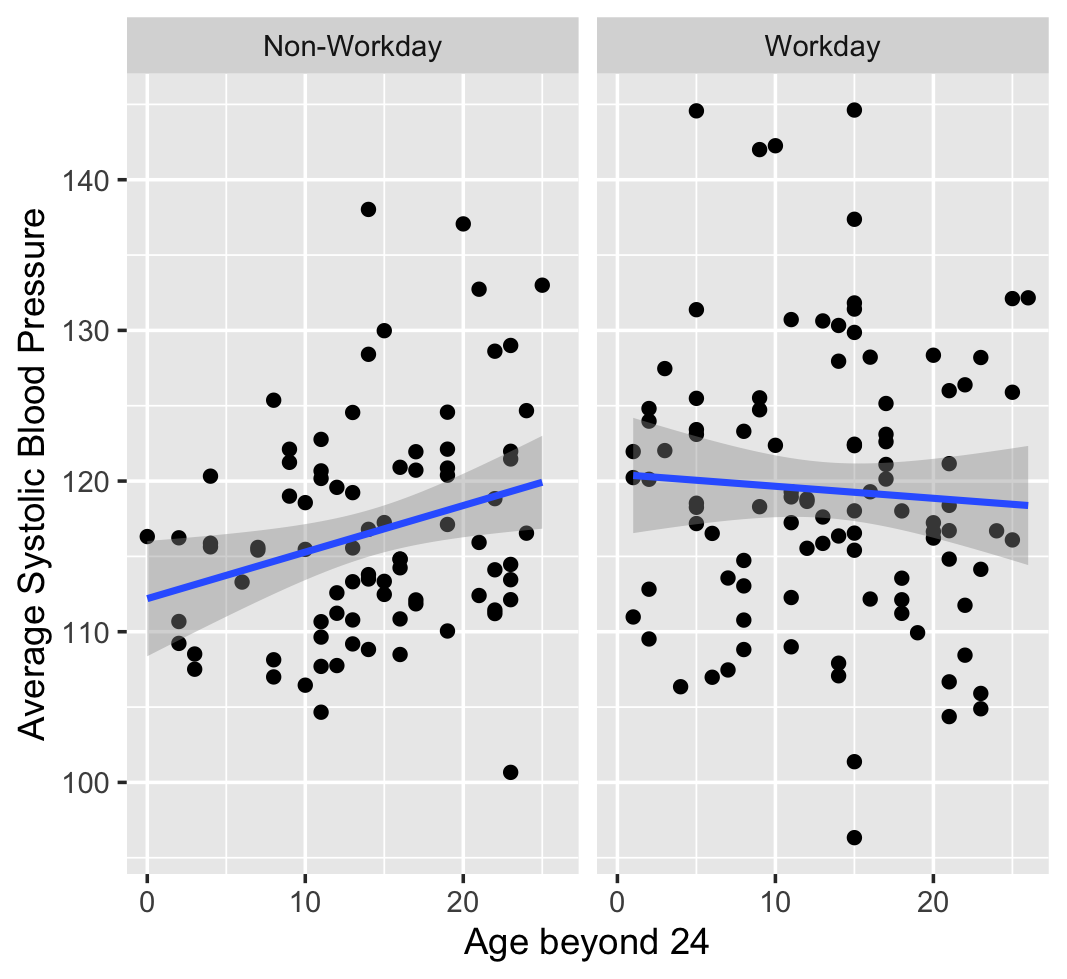
\includegraphics[width=\textwidth]{pics/bp by age and day.png}
        \caption[]%
        {{\small BP vs. Age Level by Workday}}
        \label{fig: bp v age and day}
        \end{subfigure}
        \hfill
        \begin{subfigure}[b]{0.3\textwidth}
        \centering
        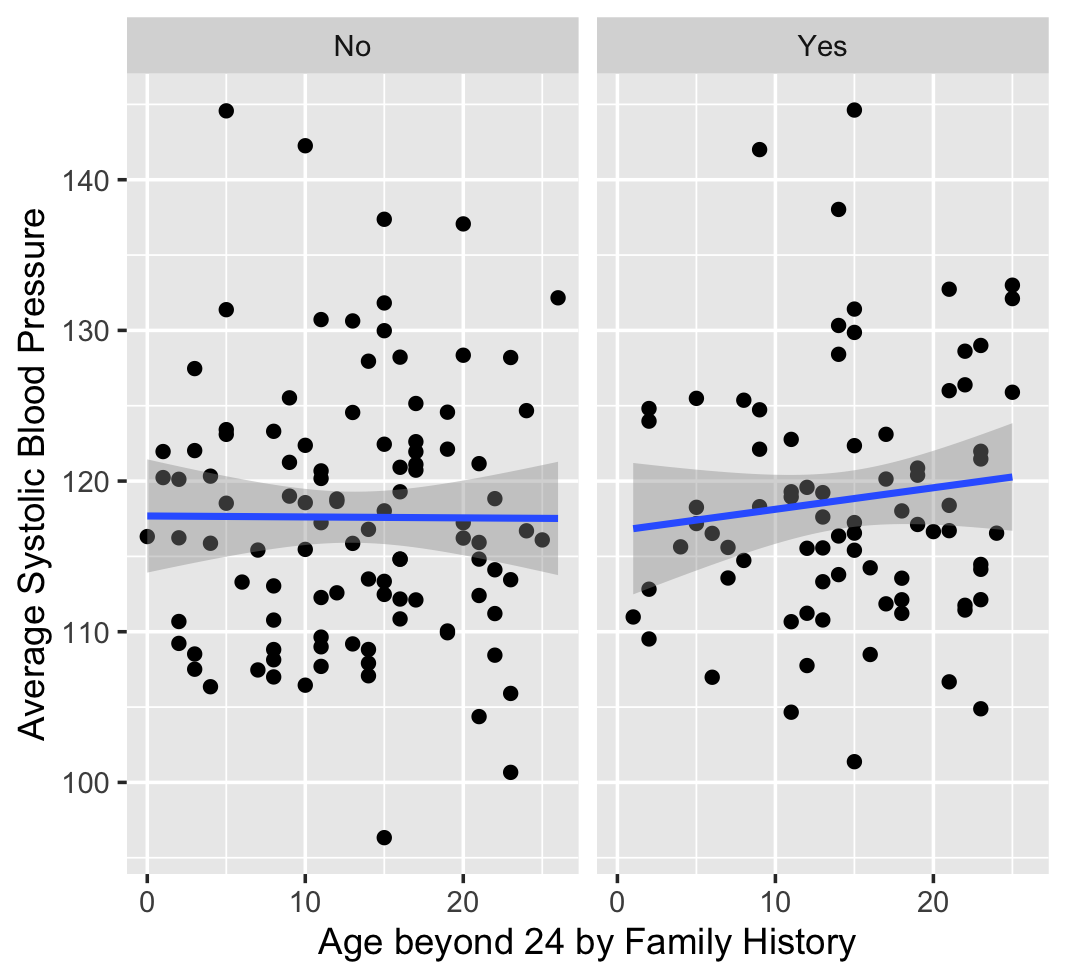
\includegraphics[width=\textwidth]{pics/bp by age and fh.png}
        \caption[]%
        {{\small BP vs. Age by Family History}}
        \label{fig: bp v age and fh}
        \end{subfigure}
        \hfill
        \begin{subfigure}[b]{0.3\textwidth}
        \centering
        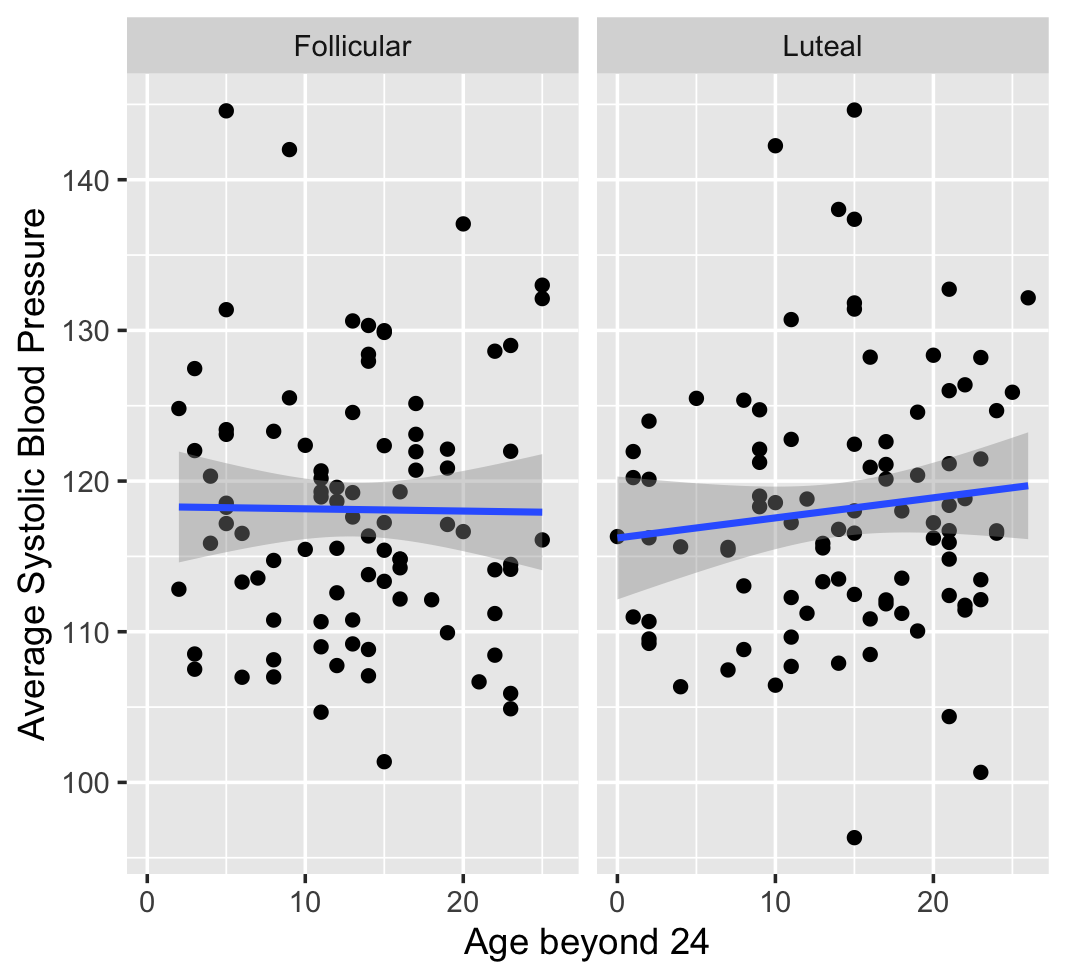
\includegraphics[width=\textwidth]{pics/bp by age and phase.png}
        \caption[]%
        {{\small BP vs. Age by Menstrual Phase}}
        \label{fig: bp v age and phase}
        \end{subfigure}
        \caption[]
        {\small BP vs. Age}
        \label{fig: bp v age and lv 2}
        \end{figure}

    \begin{figure}[h] 
        \centering
        \begin{subfigure}[b]{\textwidth}
            \centering
            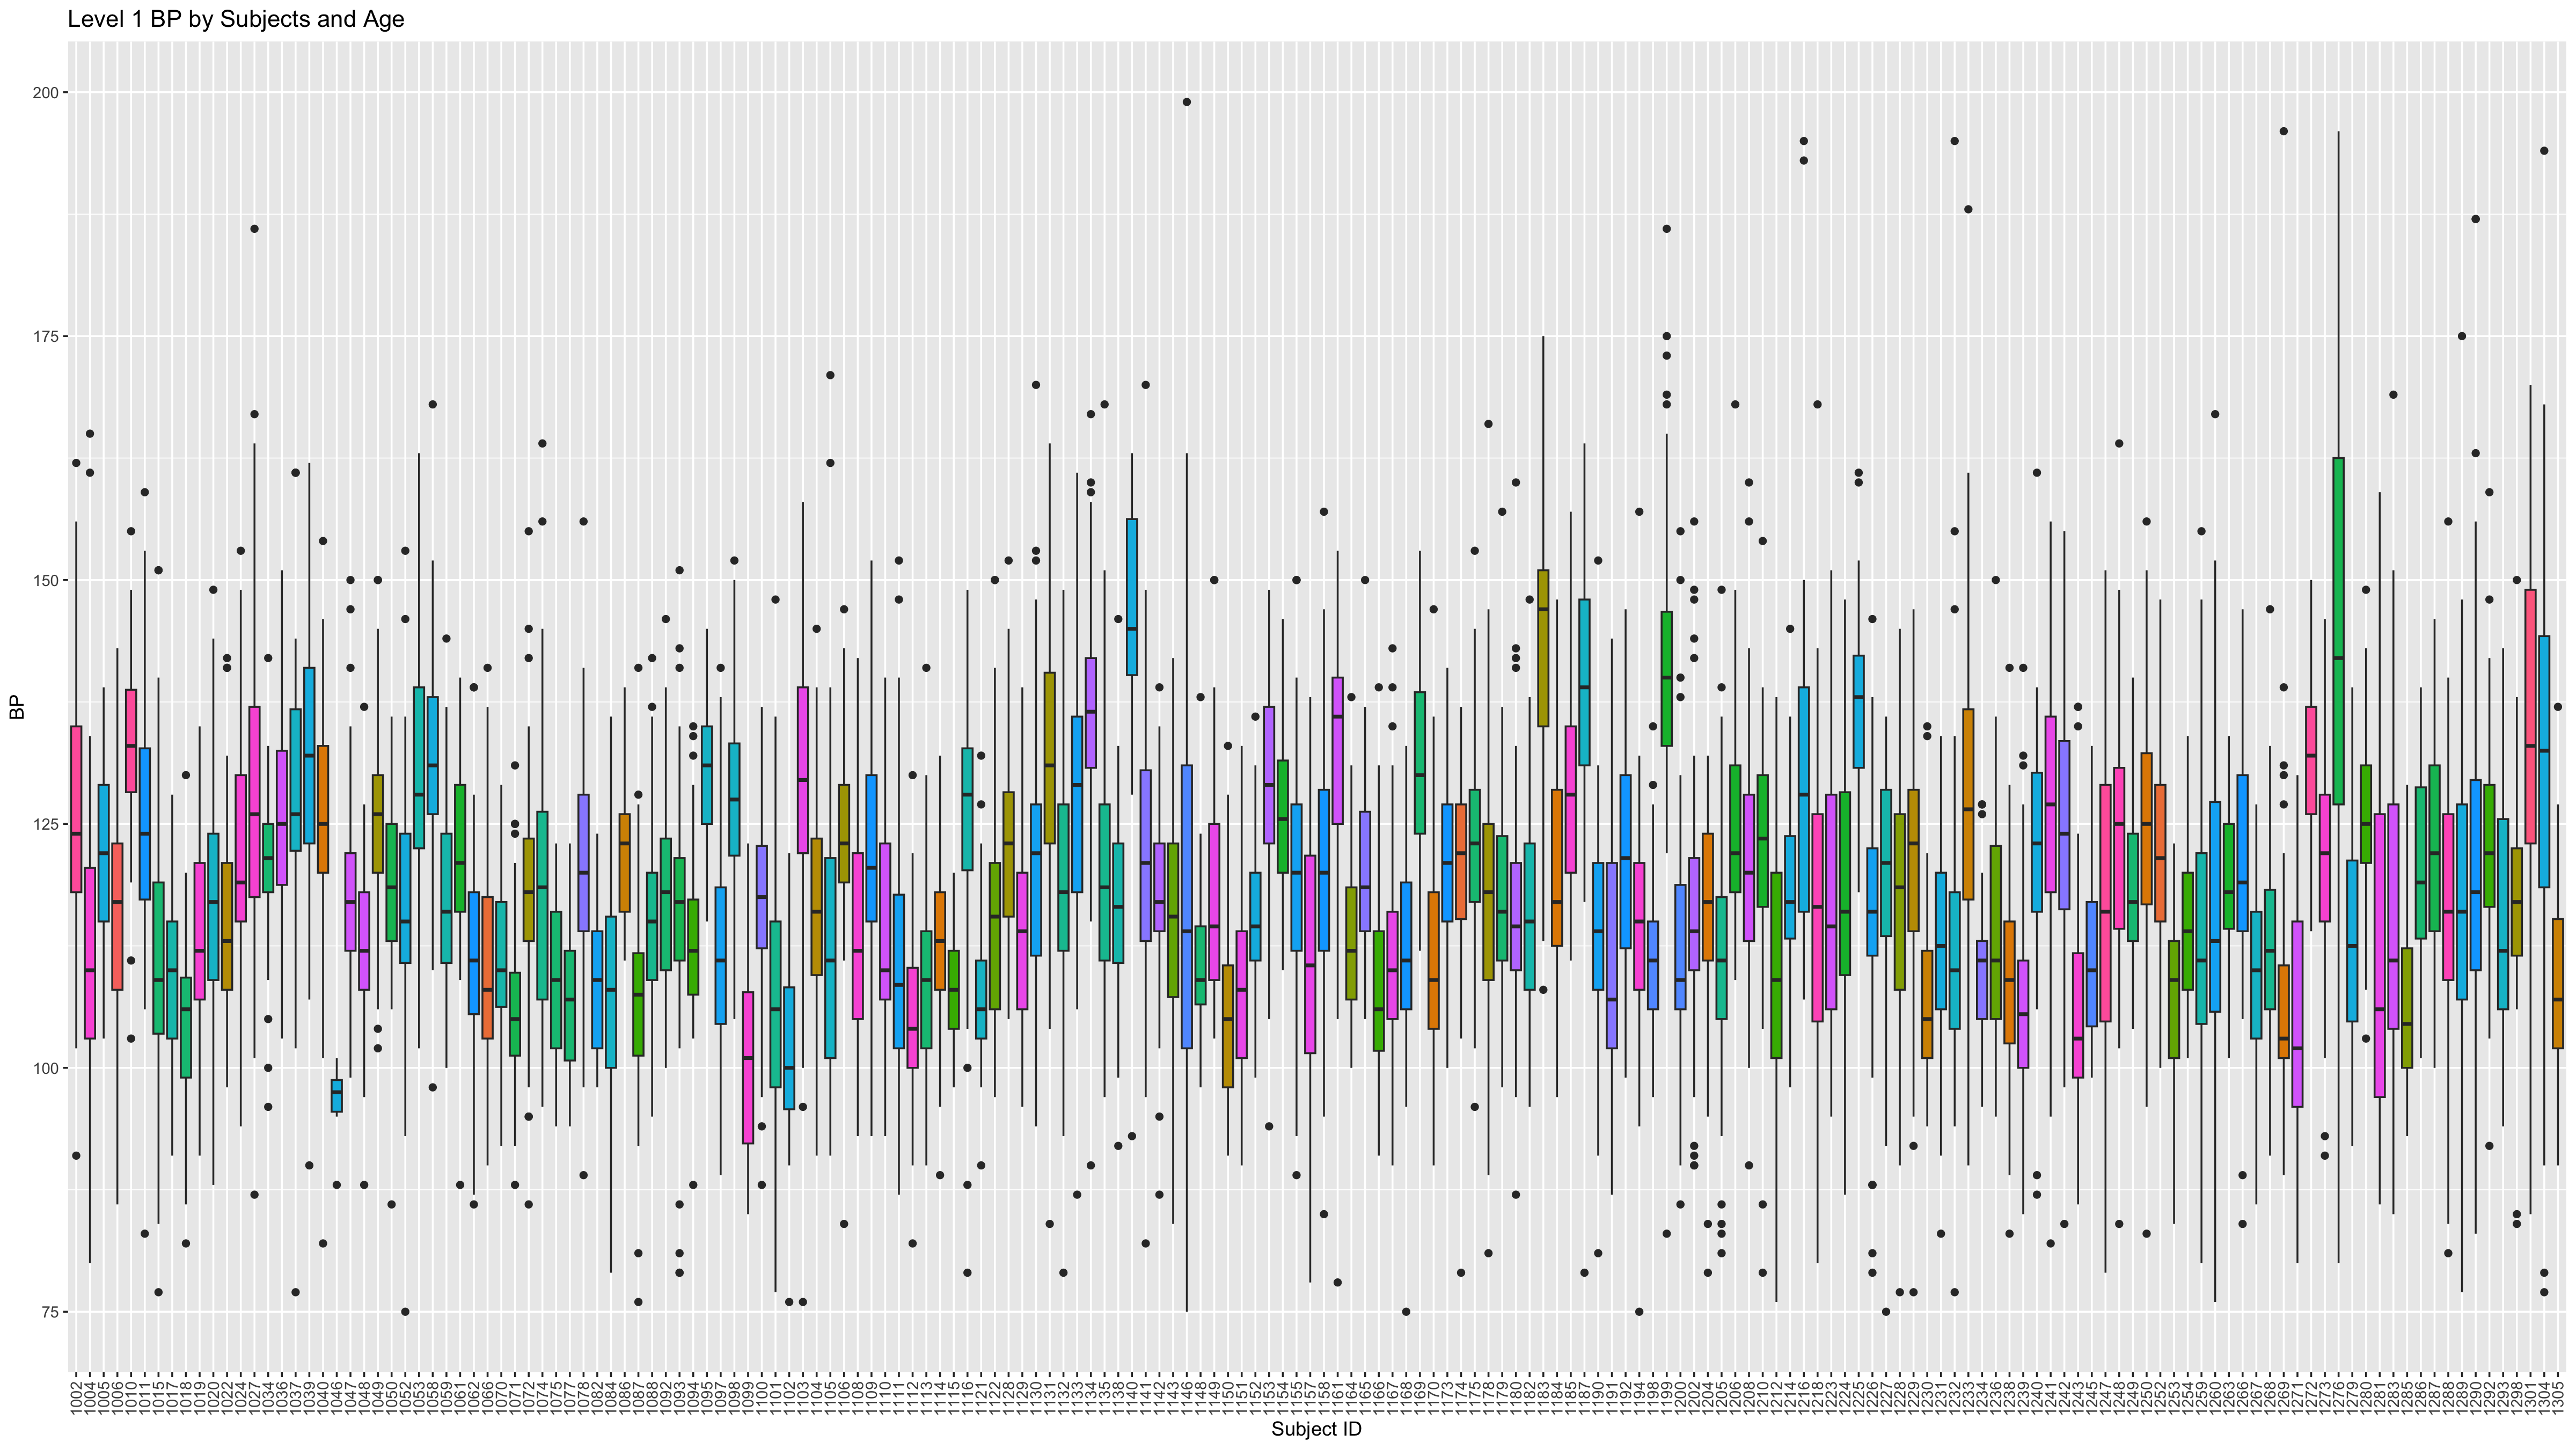
\includegraphics[width=\textwidth]{pics/bp by id and age.png}
            \caption{BP vs. Age by Subjects}
            \label{fig: bp v id and age}
        \end{subfigure}
        \caption{BP vs. Level 2}
        \label{fig: bp v id and level2_1}
    \end{figure}

    \begin{figure}[h] \ContinuedFloat
        \centering
        \begin{subfigure}[b]{\textwidth}
            \centering
            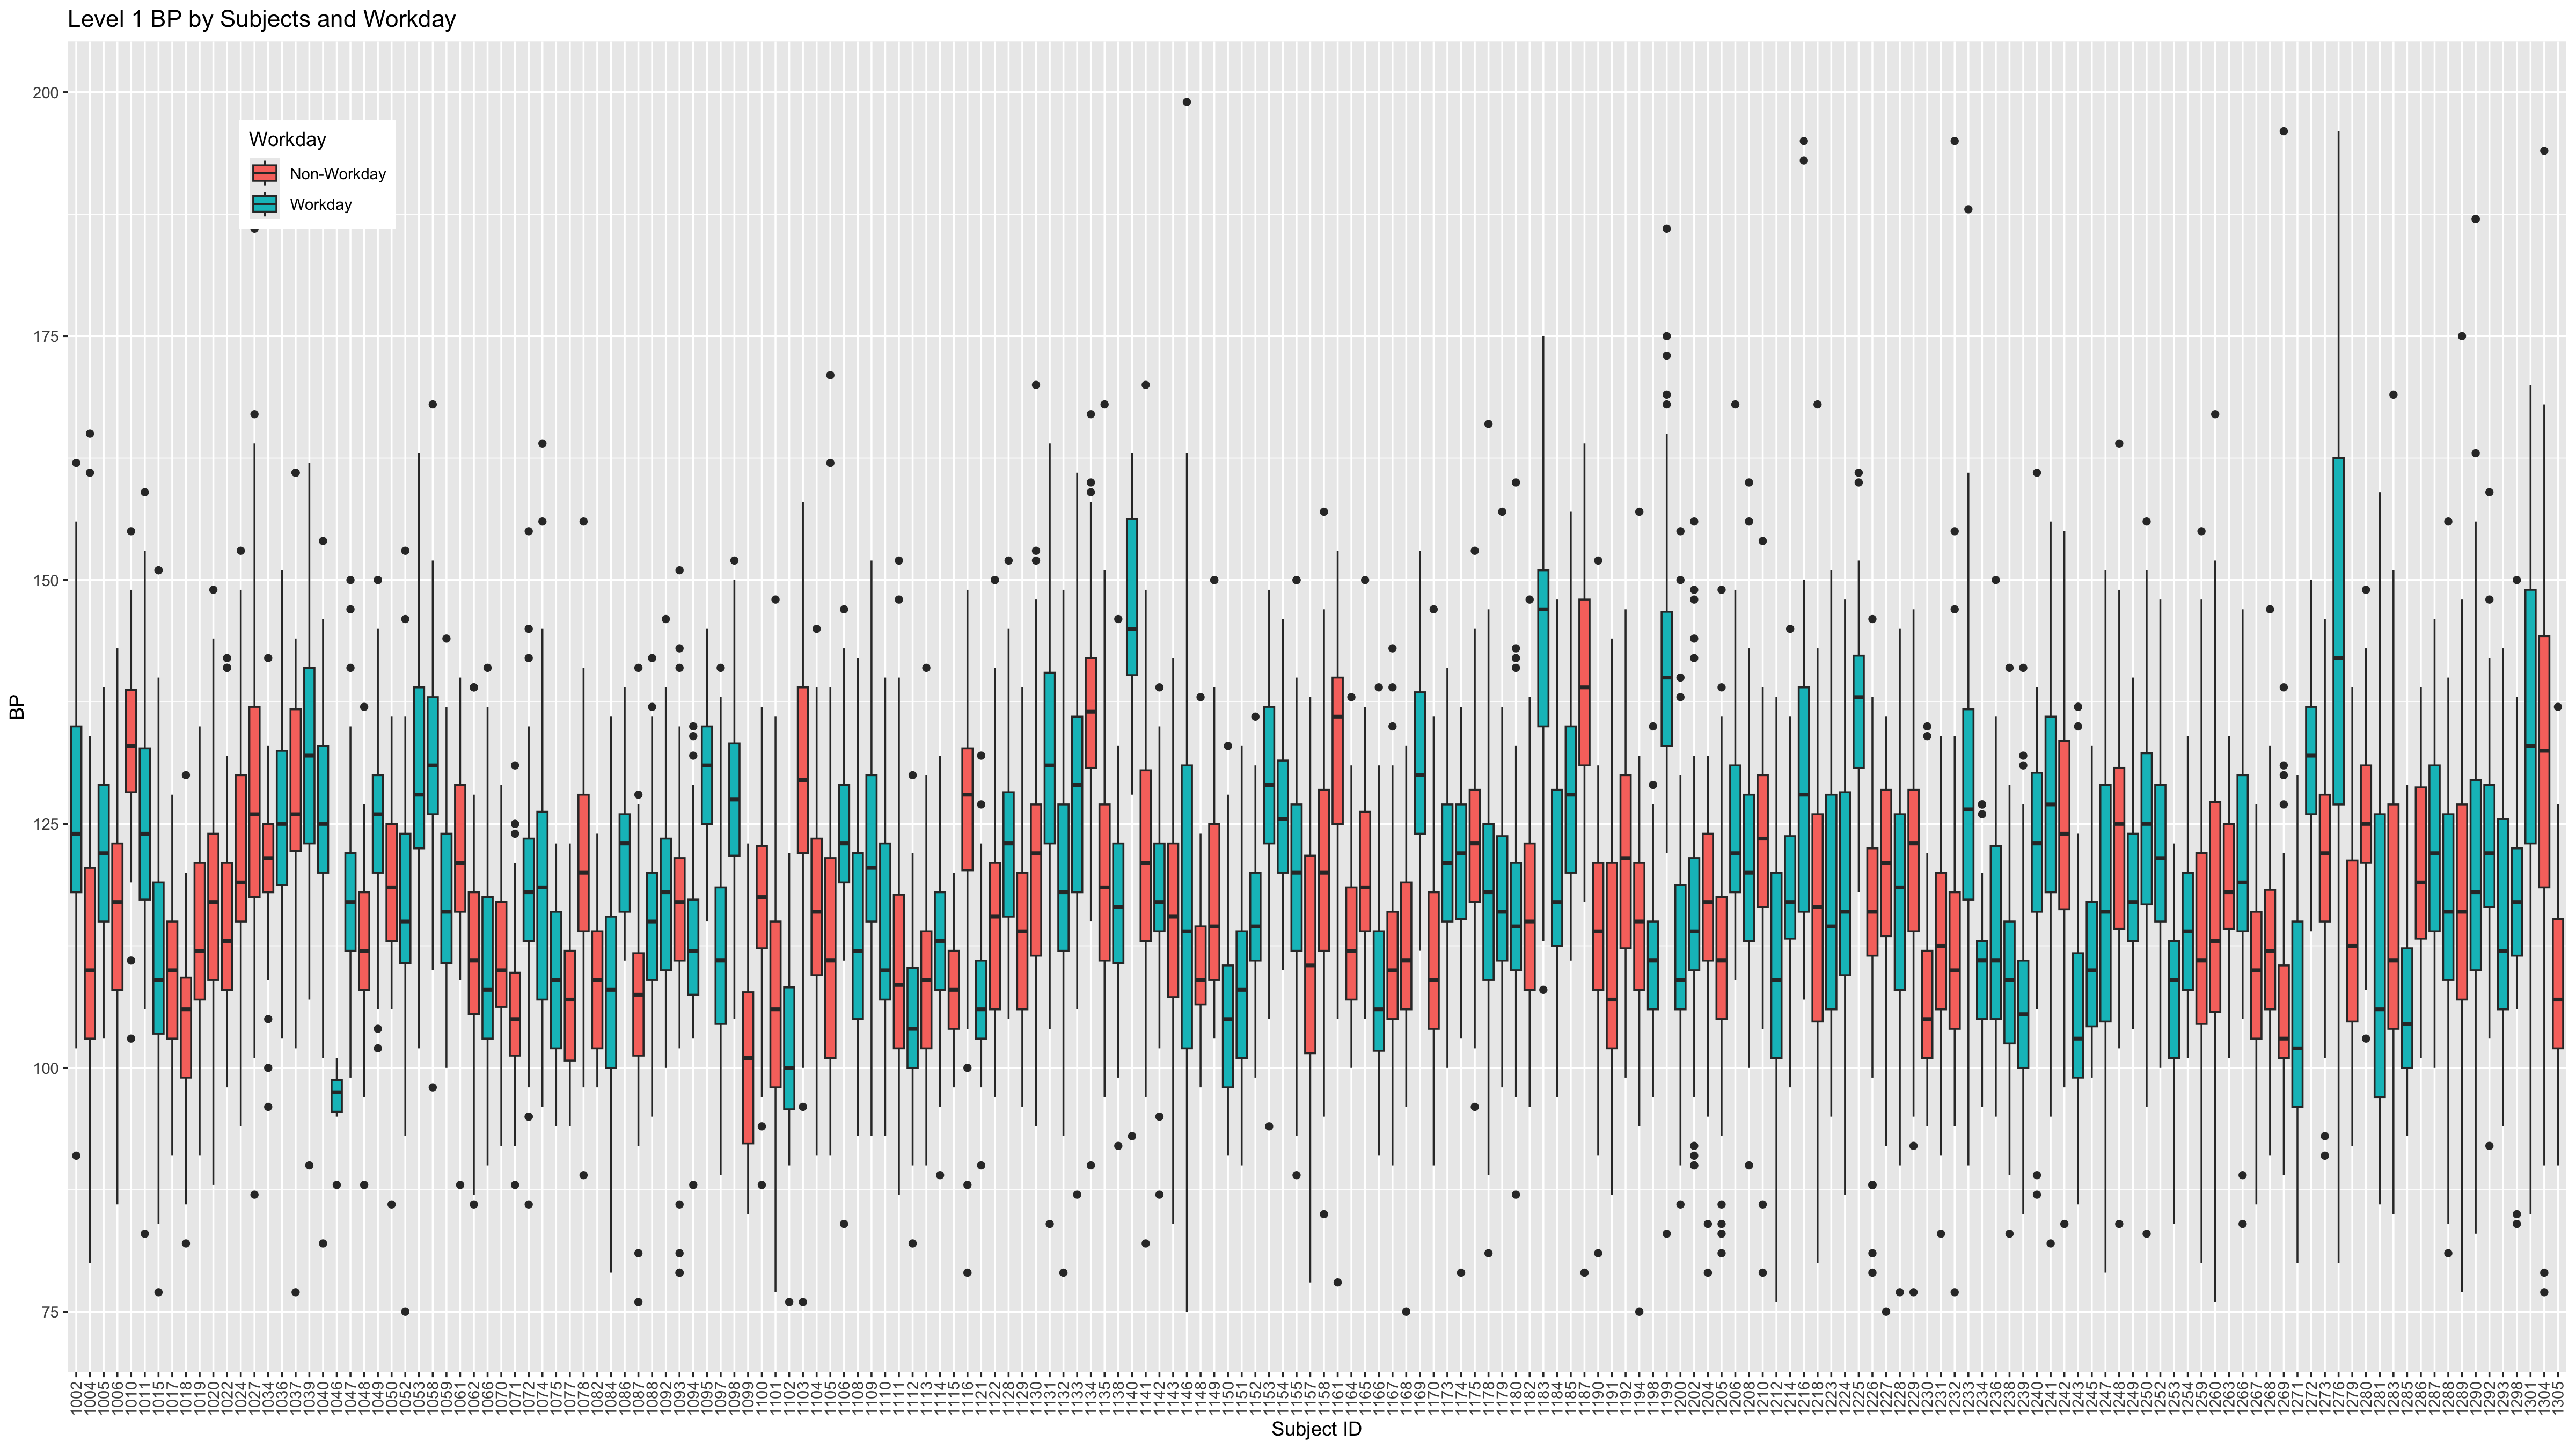
\includegraphics[width=\textwidth]{pics/bp by id and day.png}
            \caption{BP vs. Workday by Subjects}
            \label{fig: bp v id and day}
        \end{subfigure}
        \caption{BP vs. Level 2}
        \label{fig: bp v id and level2_2}
    \end{figure}

    \begin{figure}[h] \ContinuedFloat
        \centering
        \begin{subfigure}[b]{\textwidth}
            \centering
            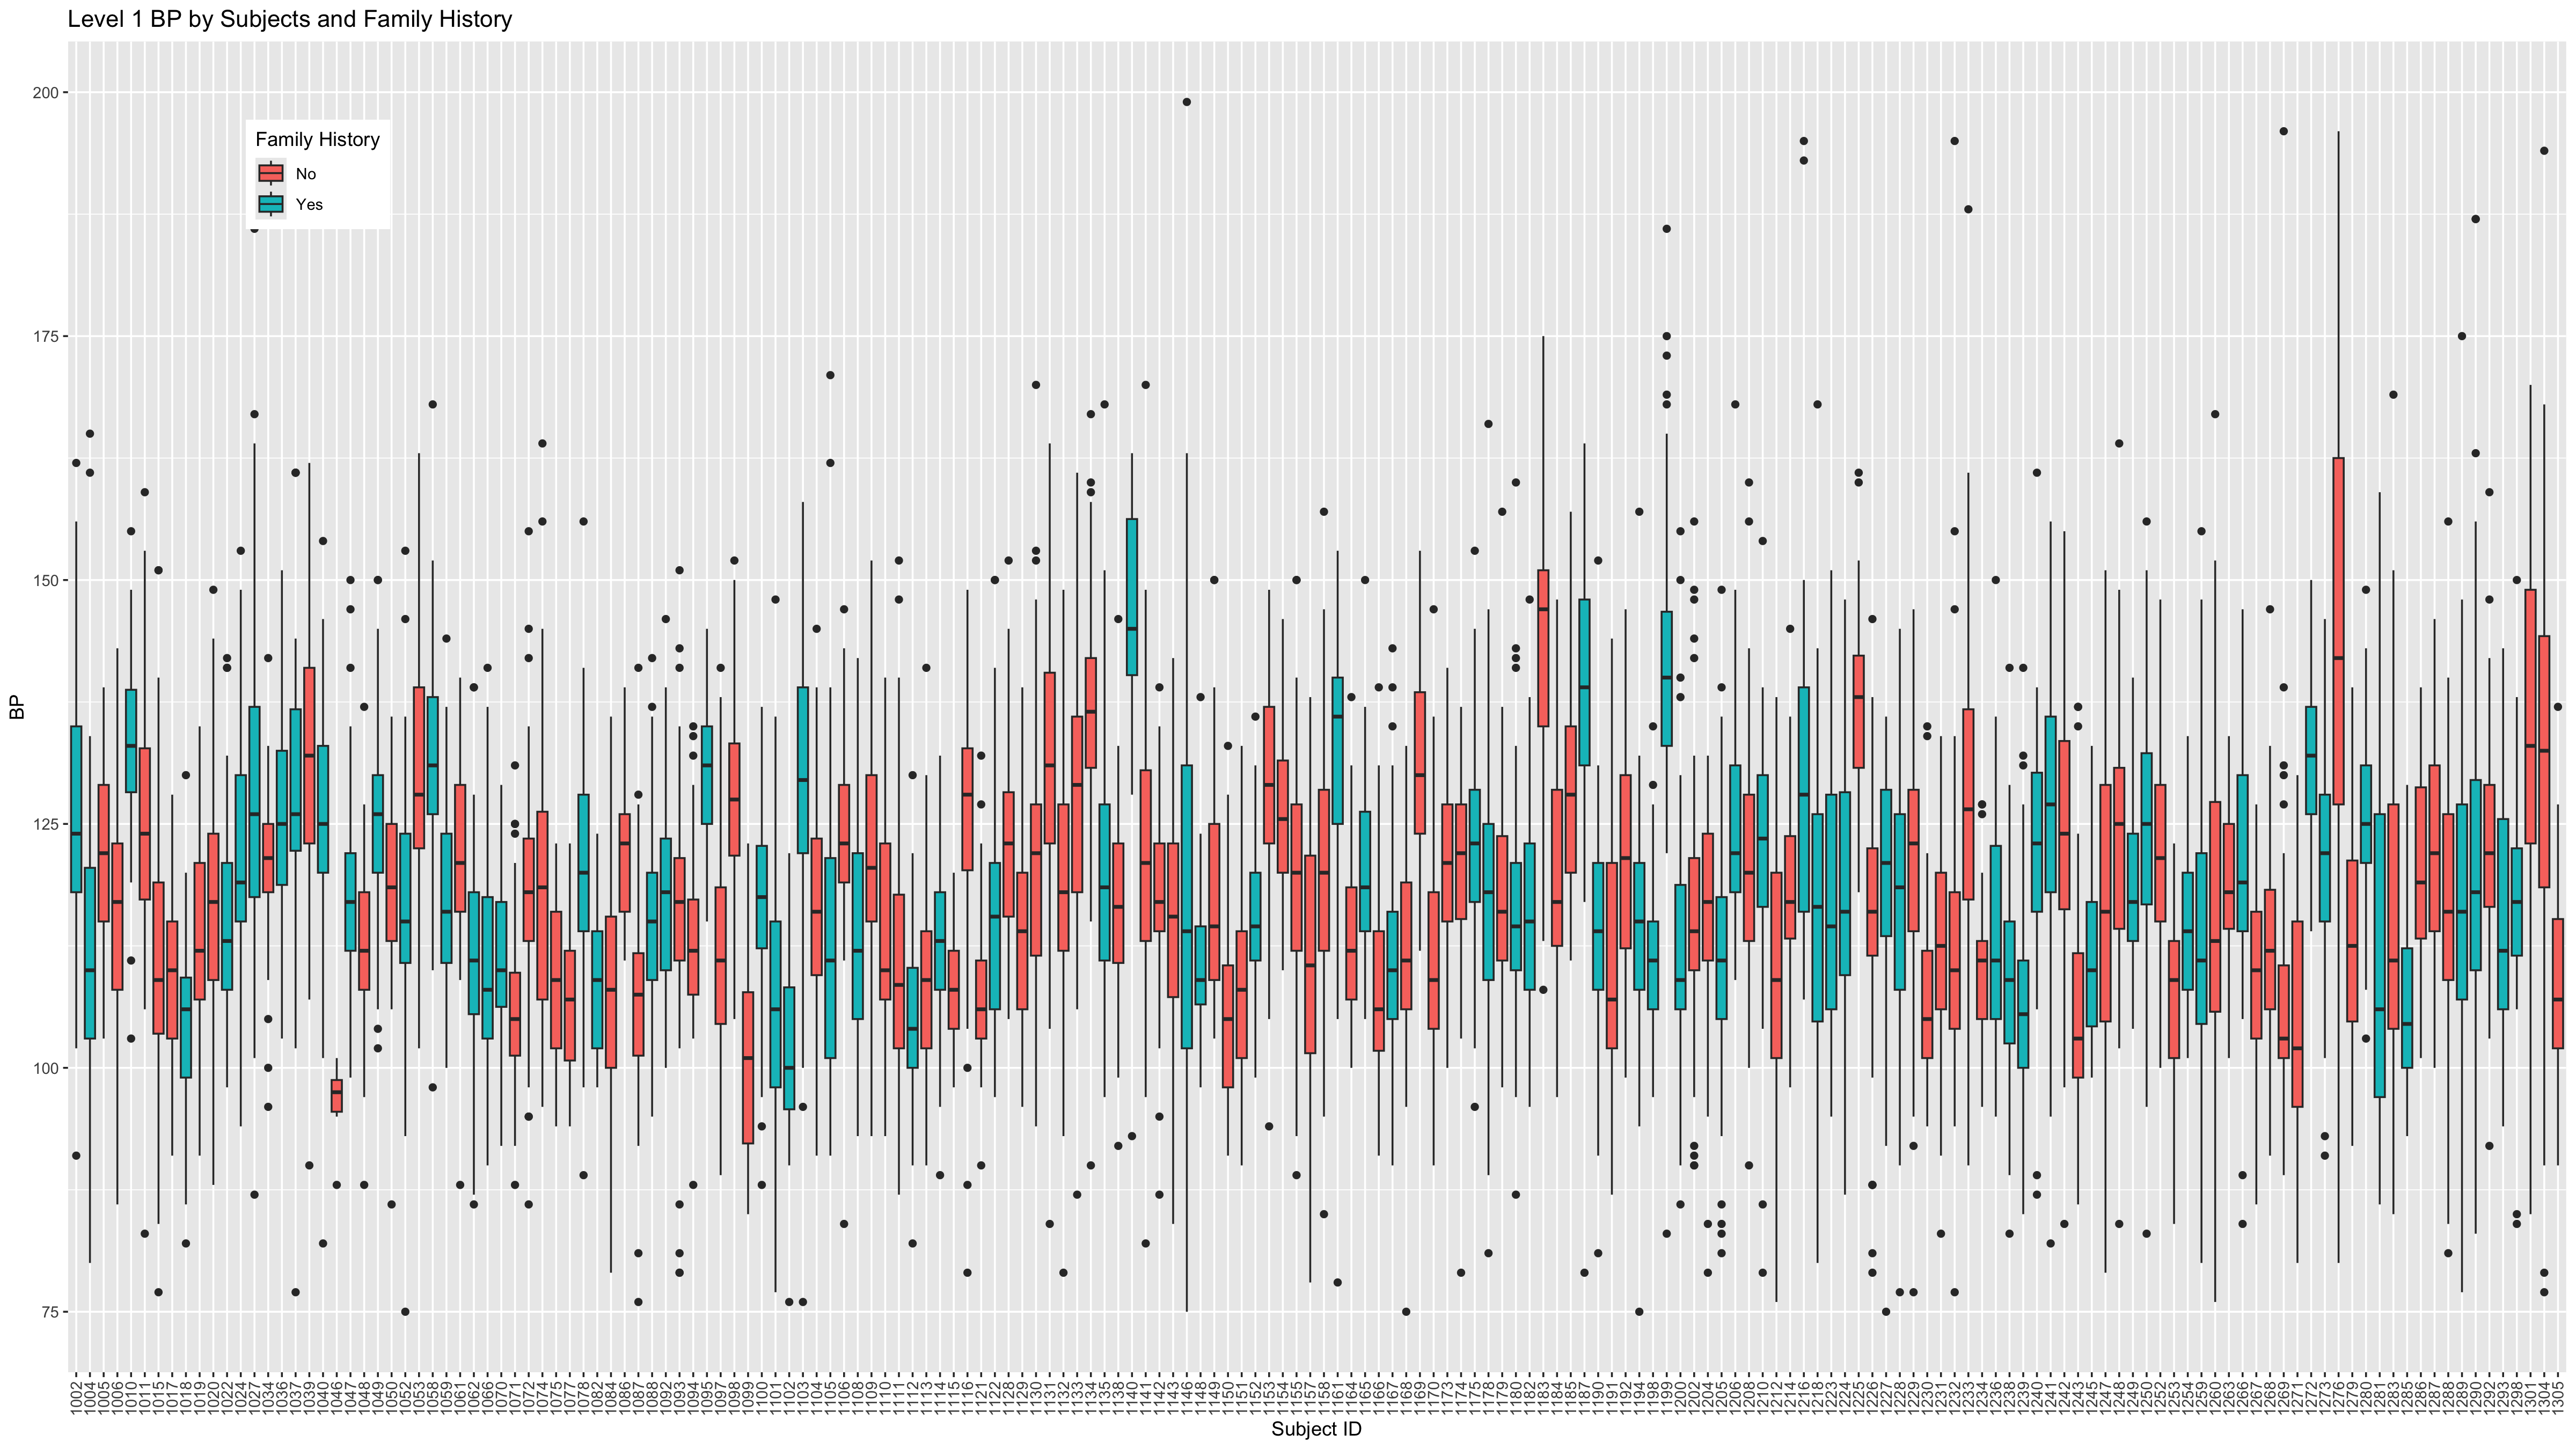
\includegraphics[width=\textwidth]{pics/bp by id and fh.png}
            \caption{BP vs. Family History by Subjects}
            \label{fig: bp v id and fh}
        \end{subfigure}
        \caption{BP vs. Level 2}
        \label{fig: bp v id and level2_3}
    \end{figure}

\end{appendices}

% \pagebreak
\singlespacing
% \bibliography{sources.bib}
% \bibliographystyle{apalike}
\printbibliography
% \detailtexcount{ccpaper}
\end{document}